% Options for packages loaded elsewhere
\PassOptionsToPackage{unicode}{hyperref}
\PassOptionsToPackage{hyphens}{url}
\PassOptionsToPackage{dvipsnames,svgnames*,x11names*}{xcolor}
%
\documentclass[
  12pt,
]{book}
\usepackage{amsmath,amssymb}
\usepackage{lmodern}
\usepackage{setspace}
\usepackage{ifxetex,ifluatex}
\ifnum 0\ifxetex 1\fi\ifluatex 1\fi=0 % if pdftex
  \usepackage[T1]{fontenc}
  \usepackage[utf8]{inputenc}
  \usepackage{textcomp} % provide euro and other symbols
\else % if luatex or xetex
  \usepackage{unicode-math}
  \defaultfontfeatures{Scale=MatchLowercase}
  \defaultfontfeatures[\rmfamily]{Ligatures=TeX,Scale=1}
\fi
% Use upquote if available, for straight quotes in verbatim environments
\IfFileExists{upquote.sty}{\usepackage{upquote}}{}
\IfFileExists{microtype.sty}{% use microtype if available
  \usepackage[]{microtype}
  \UseMicrotypeSet[protrusion]{basicmath} % disable protrusion for tt fonts
}{}
\makeatletter
\@ifundefined{KOMAClassName}{% if non-KOMA class
  \IfFileExists{parskip.sty}{%
    \usepackage{parskip}
  }{% else
    \setlength{\parindent}{0pt}
    \setlength{\parskip}{6pt plus 2pt minus 1pt}}
}{% if KOMA class
  \KOMAoptions{parskip=half}}
\makeatother
\usepackage{xcolor}
\IfFileExists{xurl.sty}{\usepackage{xurl}}{} % add URL line breaks if available
\IfFileExists{bookmark.sty}{\usepackage{bookmark}}{\usepackage{hyperref}}
\hypersetup{
  pdftitle={Radiografía del Cambio Social en Chile 2016-2021},
  colorlinks=true,
  linkcolor=blue,
  filecolor=Maroon,
  citecolor=Blue,
  urlcolor=Blue,
  pdfcreator={LaTeX via pandoc}}
\urlstyle{same} % disable monospaced font for URLs
\usepackage[left=4cm, right=3cm, top=2.5cm, bottom=2.5cm]{geometry}
\usepackage{color}
\usepackage{fancyvrb}
\newcommand{\VerbBar}{|}
\newcommand{\VERB}{\Verb[commandchars=\\\{\}]}
\DefineVerbatimEnvironment{Highlighting}{Verbatim}{commandchars=\\\{\}}
% Add ',fontsize=\small' for more characters per line
\usepackage{framed}
\definecolor{shadecolor}{RGB}{248,248,248}
\newenvironment{Shaded}{\begin{snugshade}}{\end{snugshade}}
\newcommand{\AlertTok}[1]{\textcolor[rgb]{0.94,0.16,0.16}{#1}}
\newcommand{\AnnotationTok}[1]{\textcolor[rgb]{0.56,0.35,0.01}{\textbf{\textit{#1}}}}
\newcommand{\AttributeTok}[1]{\textcolor[rgb]{0.77,0.63,0.00}{#1}}
\newcommand{\BaseNTok}[1]{\textcolor[rgb]{0.00,0.00,0.81}{#1}}
\newcommand{\BuiltInTok}[1]{#1}
\newcommand{\CharTok}[1]{\textcolor[rgb]{0.31,0.60,0.02}{#1}}
\newcommand{\CommentTok}[1]{\textcolor[rgb]{0.56,0.35,0.01}{\textit{#1}}}
\newcommand{\CommentVarTok}[1]{\textcolor[rgb]{0.56,0.35,0.01}{\textbf{\textit{#1}}}}
\newcommand{\ConstantTok}[1]{\textcolor[rgb]{0.00,0.00,0.00}{#1}}
\newcommand{\ControlFlowTok}[1]{\textcolor[rgb]{0.13,0.29,0.53}{\textbf{#1}}}
\newcommand{\DataTypeTok}[1]{\textcolor[rgb]{0.13,0.29,0.53}{#1}}
\newcommand{\DecValTok}[1]{\textcolor[rgb]{0.00,0.00,0.81}{#1}}
\newcommand{\DocumentationTok}[1]{\textcolor[rgb]{0.56,0.35,0.01}{\textbf{\textit{#1}}}}
\newcommand{\ErrorTok}[1]{\textcolor[rgb]{0.64,0.00,0.00}{\textbf{#1}}}
\newcommand{\ExtensionTok}[1]{#1}
\newcommand{\FloatTok}[1]{\textcolor[rgb]{0.00,0.00,0.81}{#1}}
\newcommand{\FunctionTok}[1]{\textcolor[rgb]{0.00,0.00,0.00}{#1}}
\newcommand{\ImportTok}[1]{#1}
\newcommand{\InformationTok}[1]{\textcolor[rgb]{0.56,0.35,0.01}{\textbf{\textit{#1}}}}
\newcommand{\KeywordTok}[1]{\textcolor[rgb]{0.13,0.29,0.53}{\textbf{#1}}}
\newcommand{\NormalTok}[1]{#1}
\newcommand{\OperatorTok}[1]{\textcolor[rgb]{0.81,0.36,0.00}{\textbf{#1}}}
\newcommand{\OtherTok}[1]{\textcolor[rgb]{0.56,0.35,0.01}{#1}}
\newcommand{\PreprocessorTok}[1]{\textcolor[rgb]{0.56,0.35,0.01}{\textit{#1}}}
\newcommand{\RegionMarkerTok}[1]{#1}
\newcommand{\SpecialCharTok}[1]{\textcolor[rgb]{0.00,0.00,0.00}{#1}}
\newcommand{\SpecialStringTok}[1]{\textcolor[rgb]{0.31,0.60,0.02}{#1}}
\newcommand{\StringTok}[1]{\textcolor[rgb]{0.31,0.60,0.02}{#1}}
\newcommand{\VariableTok}[1]{\textcolor[rgb]{0.00,0.00,0.00}{#1}}
\newcommand{\VerbatimStringTok}[1]{\textcolor[rgb]{0.31,0.60,0.02}{#1}}
\newcommand{\WarningTok}[1]{\textcolor[rgb]{0.56,0.35,0.01}{\textbf{\textit{#1}}}}
\usepackage{longtable,booktabs,array}
\usepackage{calc} % for calculating minipage widths
% Correct order of tables after \paragraph or \subparagraph
\usepackage{etoolbox}
\makeatletter
\patchcmd\longtable{\par}{\if@noskipsec\mbox{}\fi\par}{}{}
\makeatother
% Allow footnotes in longtable head/foot
\IfFileExists{footnotehyper.sty}{\usepackage{footnotehyper}}{\usepackage{footnote}}
\makesavenoteenv{longtable}
\usepackage{graphicx}
\makeatletter
\def\maxwidth{\ifdim\Gin@nat@width>\linewidth\linewidth\else\Gin@nat@width\fi}
\def\maxheight{\ifdim\Gin@nat@height>\textheight\textheight\else\Gin@nat@height\fi}
\makeatother
% Scale images if necessary, so that they will not overflow the page
% margins by default, and it is still possible to overwrite the defaults
% using explicit options in \includegraphics[width, height, ...]{}
\setkeys{Gin}{width=\maxwidth,height=\maxheight,keepaspectratio}
% Set default figure placement to htbp
\makeatletter
\def\fps@figure{htbp}
\makeatother
\setlength{\emergencystretch}{3em} % prevent overfull lines
\providecommand{\tightlist}{%
  \setlength{\itemsep}{0pt}\setlength{\parskip}{0pt}}
\setcounter{secnumdepth}{5}
\usepackage[utf8]{inputenc}
\usepackage[spanish,es-tabla]{babel}
\usepackage[fixlanguage]{babelbib}
\usepackage{geometry}
\geometry{letterpaper,left=2cm,top=2cm, right=2cm}
\usepackage{times}           
\usepackage{caption}
\captionsetup[figure, table]{labelfont={bf},labelformat={default},labelsep=period}
\usepackage{graphicx}
\usepackage{booktabs}
\usepackage{longtable}
\usepackage{array}
\usepackage{multirow}
\usepackage{wrapfig}
%\usepackage{float}
\usepackage{colortbl}
\usepackage{xcolor}
\usepackage{pdflscape}
\usepackage{tabu}
\usepackage{threeparttable}
\usepackage{pdfpages}
\usepackage{hyphsubst}
\usepackage{floatrow}
\floatsetup[figure]{capposition=top}
\floatsetup[table]{capposition=top}
\usepackage{booktabs}
\usepackage{longtable}
\usepackage{array}
\usepackage{multirow}
\usepackage{wrapfig}
\usepackage{float}
\usepackage{colortbl}
\usepackage{pdflscape}
\usepackage{tabu}
\usepackage{threeparttable}
\usepackage{threeparttablex}
\usepackage[normalem]{ulem}
\usepackage{makecell}
\usepackage{xcolor}
\ifluatex
  \usepackage{selnolig}  % disable illegal ligatures
\fi

\title{Radiografía del Cambio Social en Chile 2016-2021}
\usepackage{etoolbox}
\makeatletter
\providecommand{\subtitle}[1]{% add subtitle to \maketitle
  \apptocmd{\@title}{\par {\large #1 \par}}{}{}
}
\makeatother
\subtitle{Estudio Longitudinal Social de Chile}
\author{}
\date{\vspace{-2.5em}}

\begin{document}
\maketitle

{
\hypersetup{linkcolor=}
\setcounter{tocdepth}{1}
\tableofcontents
}
\listoftables
\listoffigures
\setstretch{1.5}
\hypertarget{introducciuxf3n}{%
\chapter*{Introducción}\label{introducciuxf3n}}
\addcontentsline{toc}{chapter}{Introducción}

El Centro de Estudios de Conflicto y Cohesión Social (\href{https://coes.cl/}{COES}) tiene el agrado de publicar el informe ``Radiografía del Cambio Social,'' el cual consolida los principales hallazgos longitudinales de cinco mediciones anuales del Estudio Longitudinal Social de Chile (\href{https://coes.cl/encuesta-panel/}{ELSOC}).

ELSOC es una encuesta desarrollada para analizar longitudinalmente, en un estudio panel, la evolución del conflicto y cohesión social en la sociedad chilena, basándose en modelos conceptuales descritos en la literatura nacional e internacional de las disciplinas del ámbito de la Economía, Sociología, Psicología, Ciencia Política y Estudios Urbanos. Se orienta a examinar los principales antecedentes, factores moderadores y mediadores, así como las principales consecuencias asociadas al desarrollo de distintas formas de sociabilidad en Chile.

Durante los últimos años, Chile se ha visto remecido por importantes eventos que han alterado aspectos sociales, políticos y económicos de la vida nacional: la pandemia asociada al COVID-19, y las consecuencias del estallido social más grande de las últimas décadas, ocurrido a partir de octubre de 2019, el que ha desencadenado un proceso constituyente inédito en la historia de Chile.

Ambos fenómenos han significado un desafío para ELSOC y para la comunidad académica, ya que afecta tanto la forma en que son levantados los datos, como las temáticas que el estudio debe abordar. Sin embargo, ELSOC presenta una oportunidad única: la posibilidad de observar el efecto que éstos fenómenos tienen sobre la población chilena desde una perspectiva longitudinal, analizando el cambio y persistencia de comportamientos, creencias y percepciones presentes en la sociedad.

Este informe se centra en tres aspectos claves de la sociedad chilena que se han visto remecidos en el último tiempo: Política y ciudadanía, donde se exploran temáticas de identificación y participación política, cambios en la relación de la ciudadanía con la política institucional y la justificación de la violencia, entre otros; Salud mental y bienestar, abarcando aspectos de salud mental y bienestar, su relación con la economía y cómo se han visto afectados a raíz de la pandemia; y Cohesión Social, donde se analiza el cambio y estabilidad del conflicto y la cohesión desde una perspectiva territorial, las actitudes y creencias de la ciudadanía en torno a los fenómenos de la migración, del sexismo y la meritocracia; entre otros.

\hypertarget{autores}{%
\section*{Autores}\label{autores}}
\addcontentsline{toc}{section}{Autores}

\begin{itemize}
\tightlist
\item
  Roberto González. \emph{Profesor Titular Escuela de Psicología PUC. Investigador Principal COES. Coordinador estudio ELSOC}
\item
  Matías Bargsted. \emph{Profesor Asociado Instituto de Sociología PUC. Investigador Asociado COES}
\item
  Ana Figuereido. \emph{Profesora titular Escuela de Psicología PUC. Investigadora Asociada COES}
\item
  Daniel Miranda. \emph{Investigador Centro Medición MIDE UC. Investigador Asociado COES}
\item
  Edgardo Cerda. \emph{Asistente Técnico ELSOC}
\item
  Alejandro Plaza. \emph{Coordinador Técnico ELSOC}
\item
  Rocío Salas-Lewin. \emph{Asistente de investigación ELSOC}
\end{itemize}

\hypertarget{investigadores-colaboradores}{%
\subsection*{Investigadores colaboradores:}\label{investigadores-colaboradores}}
\addcontentsline{toc}{subsection}{Investigadores colaboradores:}

\begin{itemize}
\tightlist
\item
  Fabián Duarte. \emph{Profesor Asociado, Escuela de Economía UCH}
\item
  Barbara Flores. \emph{Investigadora postdoctoral COES y DESOC}
\item
  Álvaro Jiménez. \emph{Profesor adjunto, Escuela de Psicología UDP}
\item
  Natalia Riquelme. \emph{Coordinadora COES}
\item
  Elisa Salas. \emph{Practicante Economía PUC}
\item
  Isidora Didier. \emph{Practicante Sociología UCH}
\item
  Cristobal Ortíz. \emph{Practicante Sociologia UCH}
\end{itemize}

\hypertarget{presentaciuxf3n-del-estudio}{%
\chapter{Presentación del estudio}\label{presentaciuxf3n-del-estudio}}

\hypertarget{sobre-coes}{%
\section{Sobre COES}\label{sobre-coes}}

El Centro de Estudios de Conflicto y Cohesión Social (\href{https://coes.cl/}{COES}) desarrolla investigación colaborativa en temas relacionados al conflicto social y la cohesión (convivencia) en Chile, por medio de un equipo multidisciplinario proveniente de las ciencias sociales y humanidades. COES centra sus actividades académicas y de difusión en el análisis de las múltiples manifestaciones del conflicto y cohesión social en Chile, sus causas, así como también su contexto cultural e histórico.

COES está patrocinado por la Universidad de Chile y la Pontificia Universidad Católica de Chile, y como instituciones asociadas se encuentran la Universidad Diego Portales y la Universidad Adolfo Ibáñez. COES cuenta con el apoyo del Fondo de Financiamiento de Centros de Investigación en Áreas Prioritarias (\href{https://www.conicyt.cl/fondap/sobre-fondap/que-es-fondap/}{FONDAP}, dependiente de la Agencia Nacional de Investigación y Desarrollo (\href{https://www.anid.cl/}{ANID}) del Ministerio de Ciencia, Tecnología, Conocimiento e Innovación (\href{https://www.minciencia.gob.cl/}{MinCiencia}). ELSOC además cuenta como socio al Instituto Milenio para la Investigación en Depresión y Personalidad (\href{https://midap.org/}{MIDAP}).

\hypertarget{sobre-elsoc}{%
\section{Sobre ELSOC}\label{sobre-elsoc}}

\hypertarget{descripciuxf3n-del-estudio}{%
\subsection*{Descripción del estudio}\label{descripciuxf3n-del-estudio}}
\addcontentsline{toc}{subsection}{Descripción del estudio}

El \href{https://coes.cl/encuesta-panel/}{Estudio Longitudinal Social de Chile (ELSOC)} es una encuesta panel, representativa de la población nacional urbana, que analiza la estabilidad y cambio de las creencias, actitudes y percepciones que tenemos los chilenos y chilenas respecto de la convivencia y del conflicto, la cohesión y una amplia gama de aspectos políticos y sociales a lo largo del tiempo.

Este estudio sigue la evolución de cerca de 4.500 chilenos y chilenas a lo largo de una década. Actualmente se encuentran disponibles 5 olas del estudio, abarcando el período entre 2016 y 2021. Sus temas de estudio y su aspecto longitudinal convierten a ELSOC en un recurso único en Chile y América Latina para analizar la evolución de la sociedad chilena y para el desarrollo de las ciencias sociales en Chile.

Durante los últimos años, ELSOC se ha consolidado como un importante insumo para el desarrollo de investigación científica y aplicada en ciencias sociales. En el sitio web de (ELSOC)(\url{https://coes.cl/encuesta-panel/}) se puede acceder a más información sobre el estudio.

\hypertarget{acceso-a-bases-de-datos-elsoc}{%
\subsection*{Acceso a Bases de Datos ELSOC}\label{acceso-a-bases-de-datos-elsoc}}
\addcontentsline{toc}{subsection}{Acceso a Bases de Datos ELSOC}

Las bases de datos y documentación correspondientes se encuentran disponibles, de manera libre y gratuita, en un repositorio de datos, al cual se podrá acceder en el link:

\url{https://dataverse.harvard.edu/dataverse/elsoc}

En este sitio se obtendrá acceso a los datos de las 5 mediciones transversales de ELSOC, así como bases longitudinales que integran las distintas mediciones. En colaboración con el Centro de Inteligencia Territorial (\href{https://cit.uai.cl/}{CIT}), se pone también a disposición las bases ELSOC-CIT. Estas bases de datos permiten combinar la información de ELSOC, y estimaciones e indicadores territoriales y geoespaciales de distinta índole, proveniente de diversas fuentes de información nacional para los períodos 2016 a 2019.

ELSOC tiene un compromiso con los más altos estándares científicos en términos de producción y análisis de datos. Dentro de esta visión global, ELSOC se guía por las principales pautas de Transparencia y Apertura en la investigación científica. Por esta misma razón, los códigos utilizados para el desarrollo de este documento se encontrarán disponibles en \url{https://github.com/edgardo-cerda/reporte-elsoc-2021}.

\hypertarget{caracteruxedsticas-del-diseuxf1o-muestral}{%
\subsection*{Características del diseño muestral}\label{caracteruxedsticas-del-diseuxf1o-muestral}}
\addcontentsline{toc}{subsection}{Características del diseño muestral}

\begin{itemize}
\item
  Unidad de Análisis: Individuos
\item
  Muestra objetivo: 3.000 individuos en muestra original (a partir de 2016) y 1.500 en muestra refresco (a partir de 2018)
\item
  Población Objetivo: Hombres y mujeres de 18 a 75 años, residentes habituales de viviendas particulares ocupadas en zonas urbanas, localizadas en 40 ciudades (92 comunas, 13 regiones) del país
\item
  Periodicidad: Anual.
\item
  Diseño Muestral: Probabilístico, estratificado (por tamaño de ciudades), por conglomerados y multietápico
\item
  Marco Muestral: Marco de muestreo de manzanas del pre-censo 2011
\item
  Unidades de Muestreo: Primero se eligen ciudades (UPM), luego manzanas (USM), y sub-bloques y viviendas (UTM). La unidad final de selección es la persona
\end{itemize}

\textbf{Organismo Ejecutor}: Consultora Stephanie Eckman y Centro de Inteligencia Territorial (CIT) de la Universidad Adolfo Ibáñez

\begin{figure}

{\centering 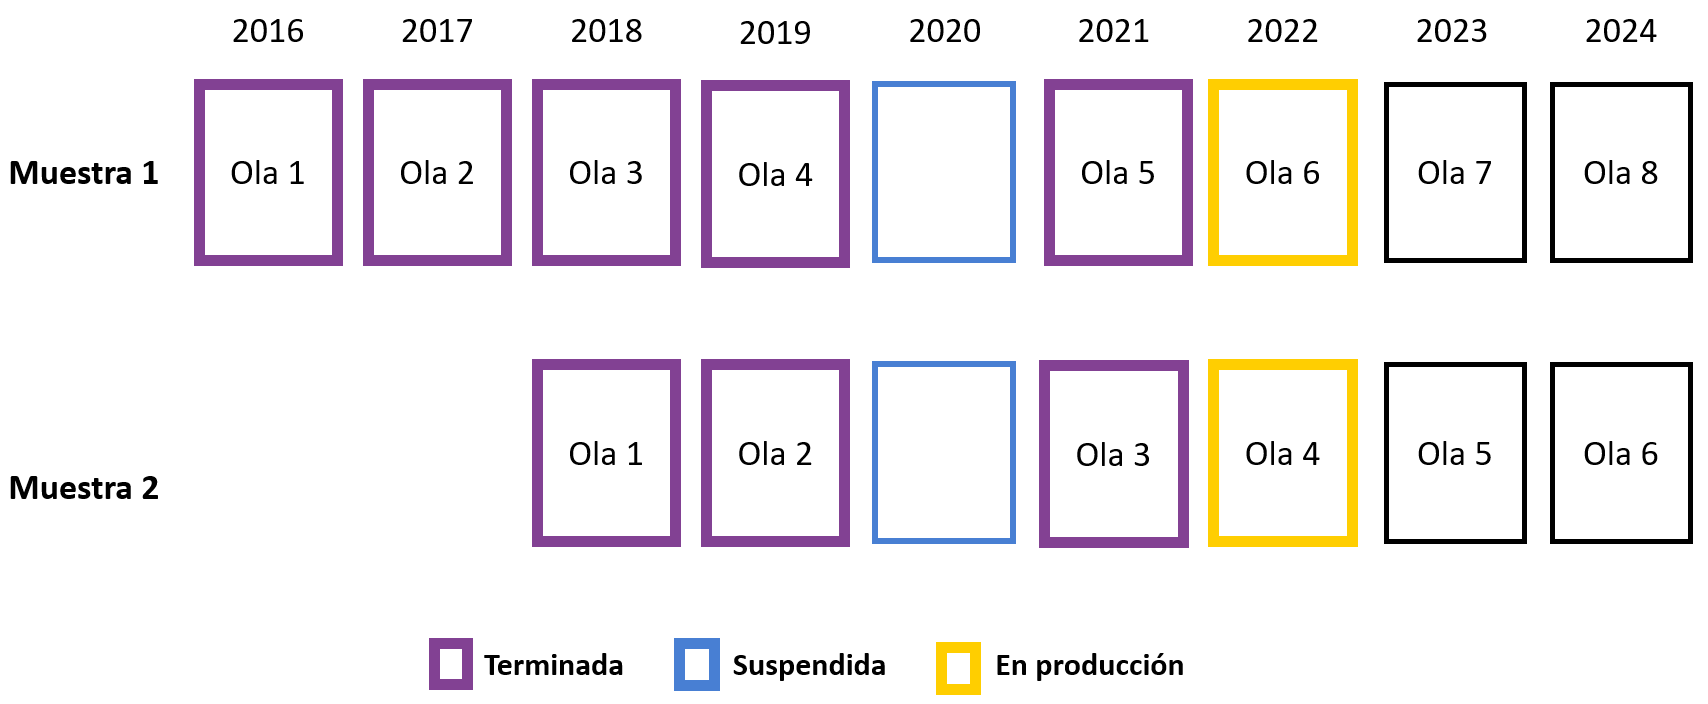
\includegraphics[width=1\linewidth,height=1\textheight]{imagenes/olas_elsoc} 

}

\caption{Mediciones de ELSOC}\label{fig:ilust-olas-elsoc}
\end{figure}

\begin{figure}

{\centering 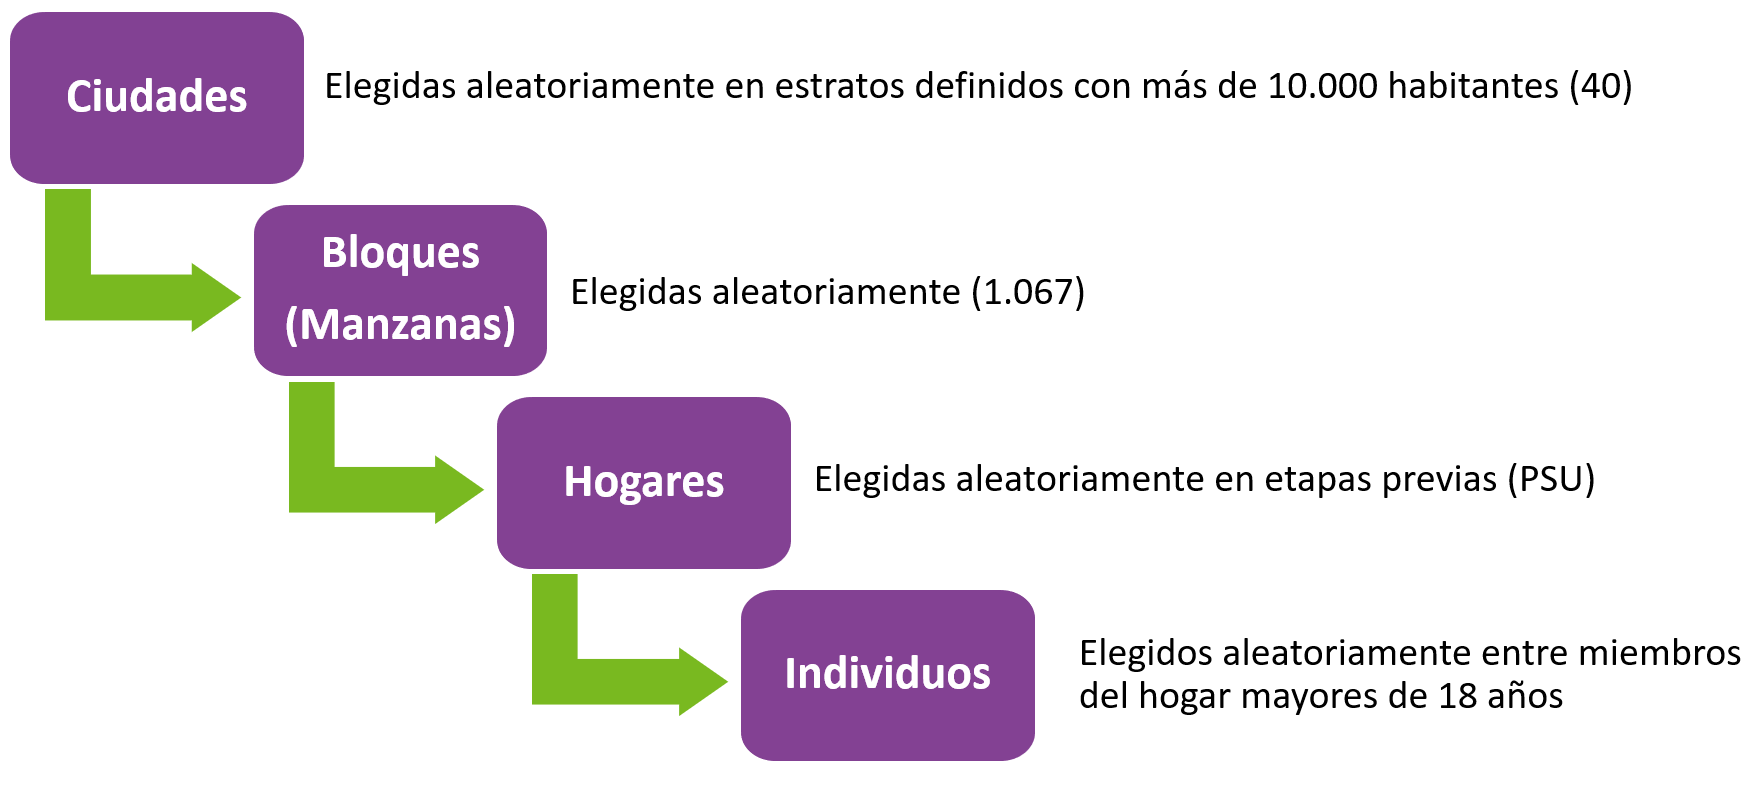
\includegraphics[width=1\linewidth,height=1\textheight]{imagenes/etapas_seleccion} 

}

\caption{Muestreo de ELSOC}\label{fig:ilust-etapas-seleccion}
\end{figure}

\hypertarget{caracteruxedsticas-del-levantamiento-de-datos}{%
\subsection*{Características del levantamiento de datos}\label{caracteruxedsticas-del-levantamiento-de-datos}}
\addcontentsline{toc}{subsection}{Características del levantamiento de datos}

\begin{itemize}
\item
  Formato de aplicación: Cuestionario estructurado. Levantamiento en formato CAPI (Encuesta presencial con asistencia de tablet). Excepcionalmente se cambió a formato CATI (Encuesta telefónica con asistencia de tablet) durante 2021, debido a contingencia COVID-19
\item
  Período de Aplicación: entre Julio y Noviembre de cada año. Debido al estallido social, la cuarta medición se aplicó entre el 21 de noviembre de 2019 y el 9 de marzo de 2020. Debido a la pandemia, la quinta medición se aplicó entre el 29 de enero de 2021 y 12 de julio de 2021
\item
  Instrumento: Cuestionario compuesto por preguntas cerradas de carácter simple y múltiple junto a algunas preguntas abiertas. Combina módulos de preguntas permanentes (medidas en todas las olas) y otras intercaladas entre olas
\item
  Cobertura Temática: Contiene siete módulos temáticos: Territorio, Redes y actitudes sociales, Ciudadanía y democracia, Desigualdad y legitimidad, Conflicto social, Salud y bienestar y Caracterización sociodemográfica
\item
  Incentivos a la participación: Entrega de incentivos monetarios para el encuestado (\$ 6.000 CLP) y de material sobre el estudio (ELSOC y COES). Acciones de seguimiento basadas en la información de contacto (correo electrónico para cumpleaños y días festivos)
\item
  Entrenamiento de entrevistadores: Contratación de entrevistadores con experiencia en encuestas complejas y/o longitudinales. Capacitación centralizada y presencial para coordinadores de campo y un subconjunto de entrevistadores en Santiago (incluidos ejercicios prácticos para la implementación del cuestionario, uso de tabletas y protocolo de contacto). Actividades adicionales en otras regiones de Chile. Diseño de un Manual de entrevistador especializado para el proyecto
\item
  Operaciones de Control y Supervisión: Coordinadores de campo supervisan el trabajo de entrevistadores, verificando el número de visitas, el contacto, la identidad del participante y preguntas claves. Organismo ejecutor realiza una supervisión interna de al menos el 10\% de la muestra (entrevistando nuevamente a algunos encuestados), verificando la duración y la respuesta de los participantes
\end{itemize}

\textbf{Organismo Ejecutor}: Levantamiento a cargo de Centro Micro Datos (CMD) de la Universidad de Chile

\hypertarget{atriciuxf3n-de-la-muestra}{%
\section{Atrición de la muestra}\label{atriciuxf3n-de-la-muestra}}

El diseño de ELSOC contempló entrevistar a 3.000 personas en su muestra original y 1.500 en la muestra refresco. Sin embargo, es habitual que en encuestas panel se reduce el número de participantes, dado que algunos optan voluntariamente por dejar de participar y otras personas no pueden ser recontactadas. Este fenómeno es conocido como atrición, y pueden tener efectos nocivos sobre la utilidad de los datos longitudinales. En el caso de ELSOC, la tasa de atrición es comparativamente baja en comparación a otros estudios similares, por lo que no se considera al momento un problema significativo. A pesar de esto, el año 2018 se introduce una muestra refresco para contrarrestar el efecto de la atrición.

El año 2021, la atrición presenta un alza importante debido a la mayor dificultad que implica el levantamiento durante la pandemia de COVID-19 y al cambio de modalidad.

\begin{table}

\caption{\label{tab:tabla-atricion}Atrición de las muestras de ELSOC entre olas}
\centering
\begin{tabular}[t]{c|c|c|c|c}
\hline
\multicolumn{1}{c|}{ } & \multicolumn{2}{c|}{Muestra original} & \multicolumn{2}{c}{Muestra refresco} \\
\cline{2-3} \cline{4-5}
Medición & Muestra lograda & Atrición & Muestra lograda & Atrición\\
\hline
2016 & 2 927 &  &  & \\
\hline
2017 & 2 473 & 15.5\% &  & \\
\hline
2018 & 2 229 & 9.9\% & 1 519 & \\
\hline
2019 & 2 153 & 3.4\% & 1 264 & 16.8\%\\
\hline
2021 & 1 739 & 19.2\% & 1 001 & 20.8\%\\
\hline
\end{tabular}
\end{table}

\hypertarget{atriciuxf3n-acumulada-seguxfan-sexo-grupo-etuxe1reo-nivel-educacional-y-estrato}{%
\subsection*{Atrición acumulada según Sexo, Grupo etáreo, Nivel educacional y Estrato}\label{atriciuxf3n-acumulada-seguxfan-sexo-grupo-etuxe1reo-nivel-educacional-y-estrato}}
\addcontentsline{toc}{subsection}{Atrición acumulada según Sexo, Grupo etáreo, Nivel educacional y Estrato}

Para el cálculo de atrición acumulada se considera el período 2016-2021 para la muestra original, y el período 2018-2021 para la muestra refresco

\begin{itemize}
\tightlist
\item
  Según sexo:
\end{itemize}

\begin{table}

\caption{\label{tab:tabla-atricion-sexo}Atrición acumulada de ELSOC, según sexo}
\centering
\begin{tabular}[t]{l|c|c|c|c}
\hline
\multicolumn{1}{c|}{ } & \multicolumn{2}{c|}{Muestra lograda en 2021} & \multicolumn{2}{c}{Atrición acumulada} \\
\cline{2-3} \cline{4-5}
Sexo & Muestra original & Muestra refresco & Muestra original & Muestra refresco\\
\hline
Hombre & 628 & 376 & 46\% & 38\%\\
\hline
Mujer & 1 111 & 625 & 37\% & 31\%\\
\hline
\end{tabular}
\end{table}

\begin{itemize}
\tightlist
\item
  Según grupo etáreo:
\end{itemize}

\begin{table}

\caption{\label{tab:tabla-atricion-edad}Atrición acumulada de ELSOC, según grupo etáreo}
\centering
\begin{tabular}[t]{l|c|c|c|c}
\hline
\multicolumn{1}{c|}{ } & \multicolumn{2}{c|}{Muestra lograda en 2021} & \multicolumn{2}{c}{Atrición acumulada} \\
\cline{2-3} \cline{4-5}
Grupo etáreo & Muestra original & Muestra refresco & Muestra original & Muestra refresco\\
\hline
18-29 & 142 & 173 & 72\% & 49\%\\
\hline
30-49 & 637 & 396 & 45\% & 32\%\\
\hline
50-64 & 609 & 291 & 27\% & 30\%\\
\hline
65 o más & 351 & 141 & 17\% & 22\%\\
\hline
\end{tabular}
\end{table}

\begin{itemize}
\tightlist
\item
  Según nivel educacional:
\end{itemize}

\begin{table}

\caption{\label{tab:tabla-atricion-educ}Atrición acumulada de ELSOC, según nivel educacional}
\centering
\begin{tabular}[t]{l|c|c|c|c}
\hline
\multicolumn{1}{c|}{ } & \multicolumn{2}{c|}{Muestra lograda en 2021} & \multicolumn{2}{c}{Atrición acumulada} \\
\cline{2-3} \cline{4-5}
Nivel educacional & Muestra original & Muestra refresco & Muestra original & Muestra refresco\\
\hline
Basica & 365 & 176 & 44\% & 38\%\\
\hline
Media & 767 & 406 & 39\% & 36\%\\
\hline
Tecnica & 278 & 170 & 42\% & 33\%\\
\hline
Universitaria & 329 & 249 & 39\% & 28\%\\
\hline
\end{tabular}
\end{table}

\begin{itemize}
\tightlist
\item
  Según estrato:
\end{itemize}

\begin{table}

\caption{\label{tab:tabla-atricion-estrato}Atrición acumulada de ELSOC, según estrato}
\centering
\begin{tabular}[t]{l|c|c|c|c}
\hline
\multicolumn{1}{c|}{ } & \multicolumn{2}{c|}{Muestra lograda en 2021} & \multicolumn{2}{c}{Atrición acumulada} \\
\cline{2-3} \cline{4-5}
Estrato & Muestra original & Muestra refresco & Muestra original & Muestra refresco\\
\hline
Santiago & 409 & 262 & 43\% & 38\%\\
\hline
Valparaíso & 214 & 102 & 43\% & 34\%\\
\hline
Concepción & 256 & 138 & 35\% & 27\%\\
\hline
Ciudades
grandes & 254 & 202 & 38\% & 32\%\\
\hline
Ciudades medianas
o pequeñas & 606 & 297 & 41\% & 35\%\\
\hline
\end{tabular}
\end{table}

\hypertarget{foco-en-el-cambio-longitudinal}{%
\section{Foco en el cambio longitudinal}\label{foco-en-el-cambio-longitudinal}}

Radiografía del Cambio Social tiene como objetivo fundamental caracterizar la estabilidad y el cambio en opiniones, actitudes y conductas de los participantes a lo largo del tiempo, enfocándose en distintas dimensiones de la cohesión y conflicto en Chile.

Para el logro de dicho objetivo, el presente reporte se centrará en un subconjunto de participantes del estudio: los 1.513 entrevistados y entrevistadas que participaron en las cinco olas de ELSOC (por lo tanto, todos son parte de la muestra original). Dicha submuestra será la base empírica de los hallazgos expuestos en las siguientes secciones.

A continuación se describe a este grupo de participantes según los mismos atributos sociodemográficos (sexo, edad, educación y zona de residencia).

Los resultados presentados a continuación incorporan el diseño muestral complejo de la encuesta, por lo que incorporan los ponderadores muestrales ajustados a población regional y sexo, según estrato y conglomerado muestral.

\begin{figure}

{\centering 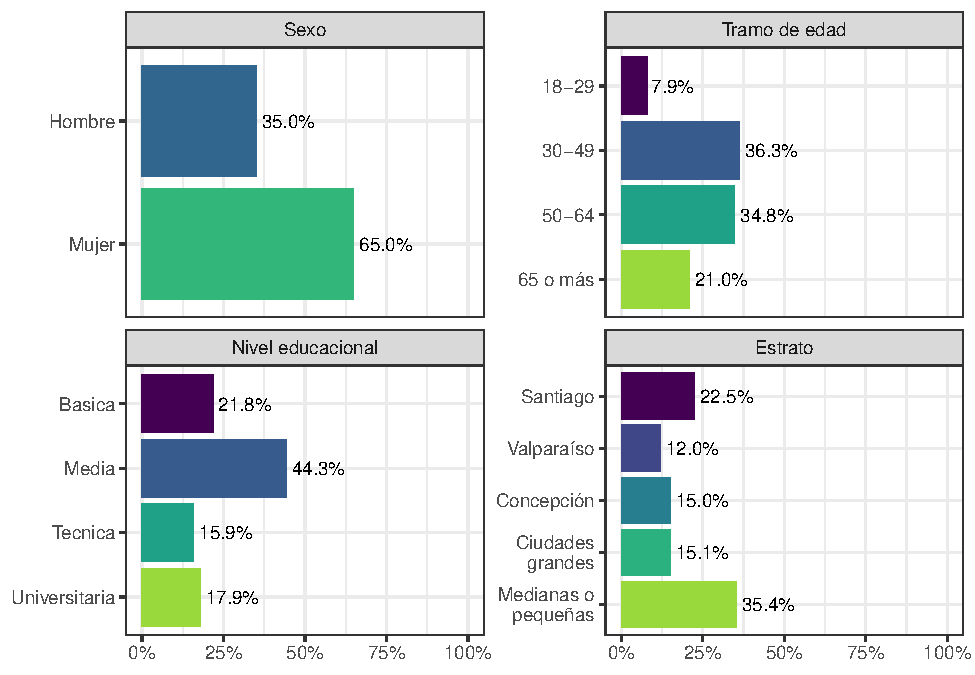
\includegraphics{reporte-elsoc_files/figure-latex/graf-composicion-muestra-1} 

}

\caption{Composición de muestra longitudinal}\label{fig:graf-composicion-muestra}
\end{figure}

\hypertarget{elsoc-en-pandemia}{%
\section{ELSOC en pandemia}\label{elsoc-en-pandemia}}

La crisis sanitaria a raíz del COVID-19 ha planteado una serie de desafíos importantes a los sistemas estadísticos a nivel general, y a las encuestas de opinión pública en particular. A partir de los planteado por la Organización Internacional del Trabajo (OIT, 2020) la mayoría de las oficinas nacionales de estadística ha informado un impacto significativo en sus operaciones, particularmente en aquellas que se llevan a cabo de manera presencial. Para sobrellevar estos problemas, varias organizaciones han tenido que transformar sus operaciones presenciales a levantamientos por teléfono o encuestas web.

Con el objetivo de asegurar la factibilidad del proceso de producción de datos de la encuesta ELSOC 2021, el equipo ejecutivo de ELSOC en conjunto con los profesionales del Centro de Microdatos de la Universidad de Chile, se decidió adoptar una serie de medidas que implicaron transitar de una modalidad presencial de producción de datos (formato CAPI) a una modalidad de producción de datos de manera remota en base a teléfono (formato CATI). En las siguientes secciones de este informe se reportan los principales cambios en ELSOC y sus implicancias.

\hypertarget{diseuxf1o-de-cuestionario-y-cambios-de-mediciuxf3n}{%
\subsection*{Diseño de cuestionario y cambios de medición}\label{diseuxf1o-de-cuestionario-y-cambios-de-mediciuxf3n}}
\addcontentsline{toc}{subsection}{Diseño de cuestionario y cambios de medición}

Durante el año 2020, se acordó con el Centro de Microdatos (CMD) que, por la medición 2021, la aplicación del cuestionario será en formato de llamada telefónica (modo CATI). Esta aplicación del cuestionario se dividió en dos llamadas de 30 minutos cada uno, para reducir el tiempo de aplicación de la entrevista, y así evitar la fatiga de los encuestados y los encuestadores (OIT, 2020).

Para evaluar los desafíos y el cambio metodológico de la aplicación, durante el 2 y 21 de diciembre de 2020 se realizó una encuesta piloto, actividad que resultó relevante para evaluar tanto los aspectos técnicos como metodológicos asociados al cambio de aplicación. En este proceso se constató la necesidad de cambiar el formato de algunas mediciones y reducir el tamaño de los cuestionarios.

En relación a la reducción de la cantidad de ítems a preguntar en el cuestionario se adoptaron los siguientes criterios:

\begin{enumerate}
\def\labelenumi{\arabic{enumi}.}
\tightlist
\item
  Reducir dimensiones que se han visto muy constreñidas por las cuarentenas, tales como participación política e interacción social
\item
  Evaluar ítems en función de la consistencia técnica y/o alineación con los objetivos de COES
\item
  Priorizar ítems que tienen menos de tres mediciones a lo largo del estudio
\item
  Mantener ítems críticos a nivel socioeconómico y de salud, que permitan realizar una buena pesquisa del impacto de la pandemia y las cuarentenas
\end{enumerate}

Por otro lado, el cambio de formato de CAPI a CATI tuvo implicancias en cómo se implementa la encuesta para los entrevistados. En esta línea se hicieron tres grandes modificaciones:

En primer lugar, y por motivos de que los encuestados ahora no disponen de un tarjetero que les permita identificar los valores de respuesta de las preguntas, es que la instrucción a los encuestadores fue que leyeran cada una de las alternativas de respuesta, de cada una de las preguntas. Esto establece un aumento sustantivo en el tiempo de respuesta del instrumento, lo que implica que un minuto de entrevista en formato CAPI no es equivalente a un minuto de respuesta de formato CATI, y por esto que se tuvo que realizar además de una separación de cuestionarios. Cabe destacar que, durante este proceso, se buscó mantener la calidad de flujo de la encuesta, resguardando variados elementos como el tiempo-eficacia de baterías de variables que compartieran un mismo encabezado inicial.

En segundo lugar, y encadenado con lo anterior, se ajustaron las variables que teniendo más de 5 categorías de respuesta generaban mayores complicaciones para preguntar en las pruebas pilotos de esta encuesta. A continuación, se presentan los ítems que fueron reducidos en sus alternativas de respuesta y el criterio que se adoptó para cada caso.

\begin{itemize}
\item
  \emph{Batería de Redes Lejanas {[}r01, r02 y r04{]}}: Esta batería consulta por la cantidad de personas en distintas ocupaciones y grupos sociales que el entrevistado conoce. Originalmente esta batería de preguntas tiene 7 valores (1. Ninguno; 2. Uno; 3. Entre 2 y 4; 4. Entre 5 y 7; 5. Entre 8 y 10; 6. Entre 11 y 15; 7. 16 o más). Debido a que los rangos de respuesta no son obedecen a un patrón claro, se tomo la decisión de preguntarles a los encuestados por el número puntual de conocidos.
\item
  \emph{Peso del entrevistado {[}s07{]}}: Esta variable presenta 9 tramos de respuesta, los cuales fueron establecidos en 5 tramos, tomando como referencia los quintiles de peso reportados por ELSOC en la ola 2018 en la variable s06
\item
  \emph{Variables de Ingreso en tramos {[}m14 y m30{]}}: La variable m14 tiene 16 tramos de respuesta, mientras que la variable m30 tiene 30 tramos de respuesta. Ambas variables fueron establecidas en 5 tramos, tomando como referencia los quintiles de ingreso presentados por la encuesta Casen 2017.
\end{itemize}

En tercer lugar, el cambio a modalidad CATI implicó que no fuera posible realizar preguntas con respuestas auto reportadas. En el caso de la ola 5, esto afectó a la batería de preguntas sobre presencia de síntomas asociados a depresión (s11\_01 a s11\_09).

Adicionalmente, cabe destacar que aproximadamente un 75\% de los encuestados fue entrevistado entre febrero y marzo de 2021 (ver Figura \ref{fig:hist-fecha-2021}), y que más del 50\% de los encuestados tuvieron 0 días de cuarentena en la comuna de residencia el mes en previo a la entrevista\footnote{Estimaciones propias basadas en fecha de respuesta y en fases de cuarentena el mes previo a la entrevista, obtenidas de \href{https://github.com/MinCiencia/Datos-COVID19}{github.com/MinCiencia/Datos-COVID19}} (ver \ref{fig:dias-cuarentena}).

\begin{figure}

{\centering 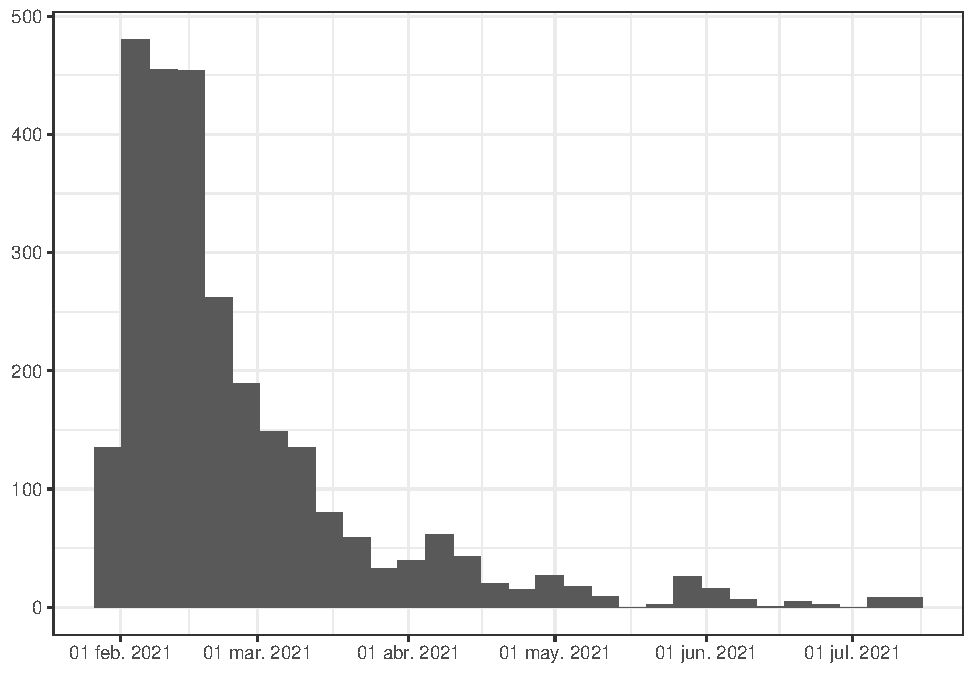
\includegraphics{reporte-elsoc_files/figure-latex/hist-fecha-2021-1} 

}

\caption{Fecha en que fueron realizadas las encuestas de la ola 2021}\label{fig:hist-fecha-2021}
\end{figure}

\begin{figure}

{\centering 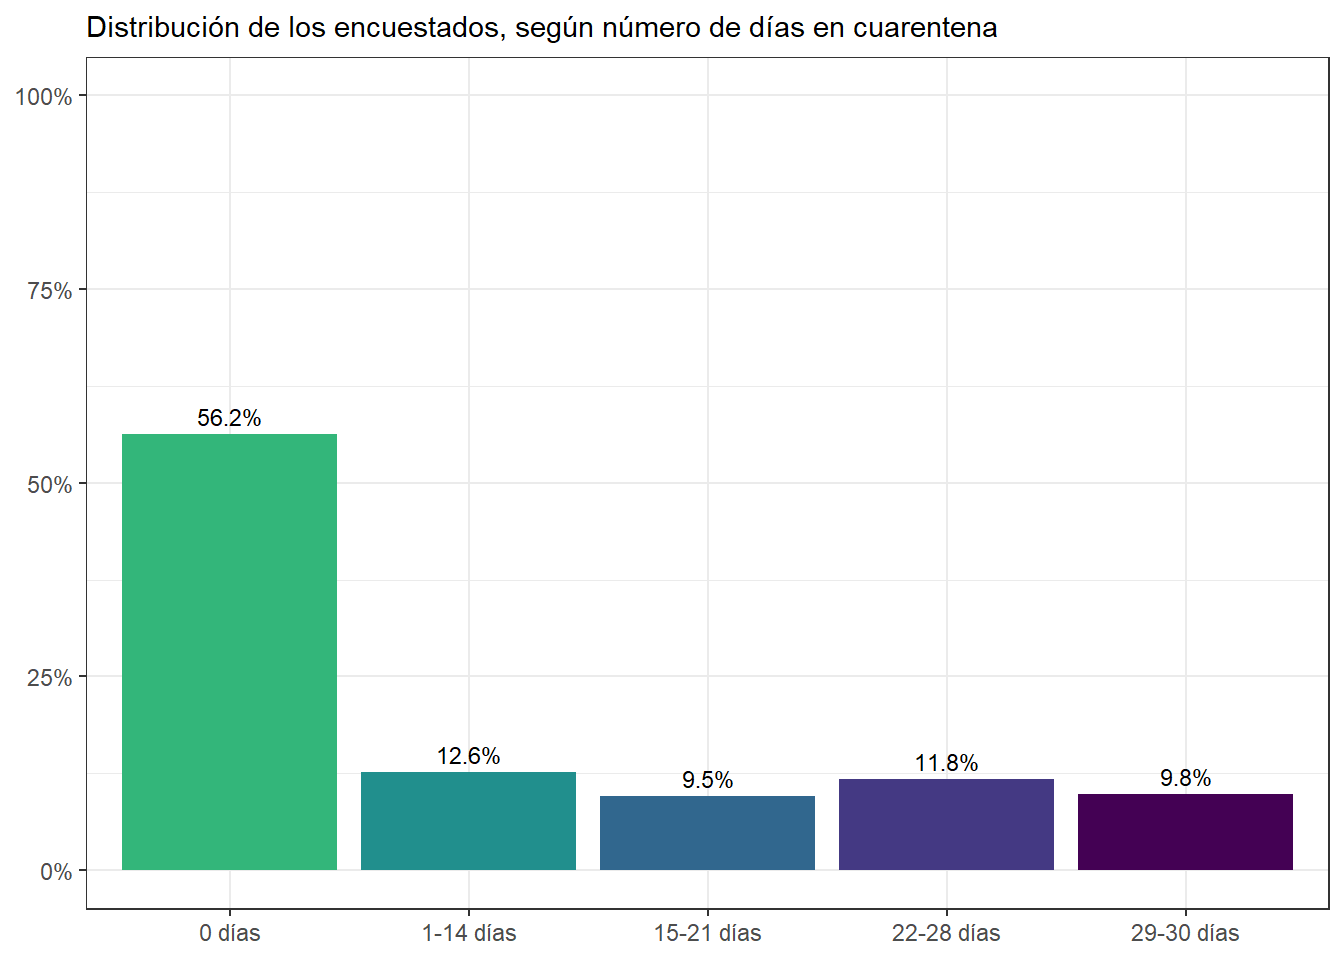
\includegraphics{reporte-elsoc_files/figure-latex/dias-cuarentena-1} 

}

\caption{Días acumulados en cuarentena, 30 días previo a la fecha de entrevista}\label{fig:dias-cuarentena}
\end{figure}

\hypertarget{poluxedtica-y-ciudadanuxeda}{%
\chapter{Política y ciudadanía}\label{poluxedtica-y-ciudadanuxeda}}

\hypertarget{identificaciuxf3n-poluxedtica}{%
\section{Identificación política}\label{identificaciuxf3n-poluxedtica}}

\hypertarget{cuxf3mo-se-posicionan-poluxedticamente-los-chilenos}{%
\subsection*{¿Cómo se posicionan políticamente los chilenos?}\label{cuxf3mo-se-posicionan-poluxedticamente-los-chilenos}}
\addcontentsline{toc}{subsection}{¿Cómo se posicionan políticamente los chilenos?}

La emergencia y consolidación en el poder de nuevas coaliciones políticas, así como la intensificación de los ciclos de protesta, hacen preguntarse por cómo ha evolucionado la identidad política de los chilenos.

La Figura \ref{fig:graf-idpolitica} muestra la foto más reciente de ELSOC acerca de cómo se distribuyen las preferencias ideológicas de la población adulta chilena, mientras que el Figura \ref{fig:graf-idpolitica-ola} muestra el cambio en las preferencias entre los años 2016 y 2021. Este último indica que la no identificación con posiciones ideológicas ha dejado de ser la respuesta mayoritaria, reafirmando al centro como la posición política con que más sujetos se identifican. Así, en 2021, por primera vez se observa que menos de un 20\% afirma no identificarse con ninguna posición del espectro izquierda-derecha, al tiempo que el centro obtiene más de un 35\% de identificación.

\begin{figure}

{\centering 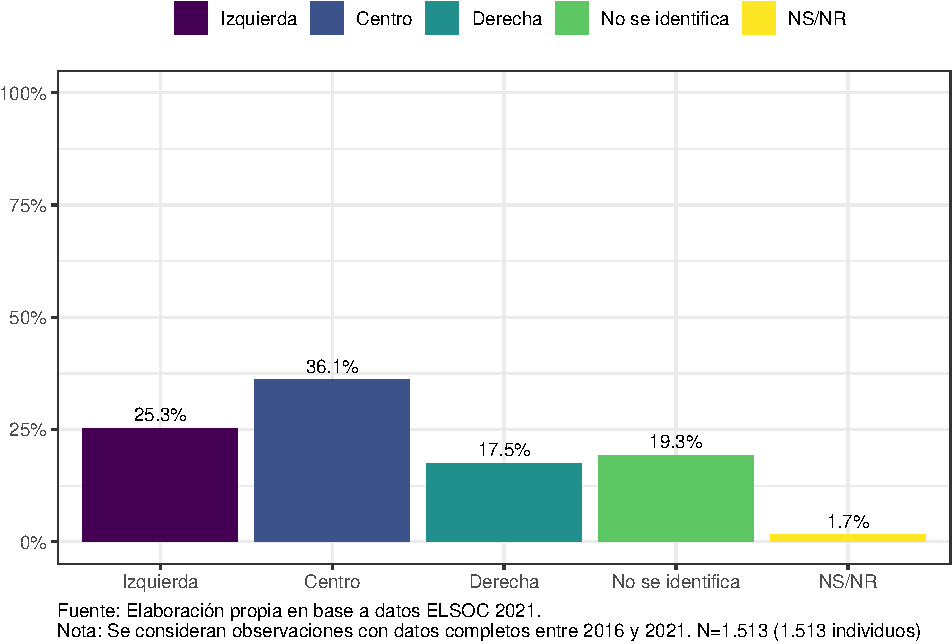
\includegraphics{reporte-elsoc_files/figure-latex/graf-idpolitica-1} 

}

\caption{Identificación política (2021)}\label{fig:graf-idpolitica}
\end{figure}

\begin{figure}

{\centering 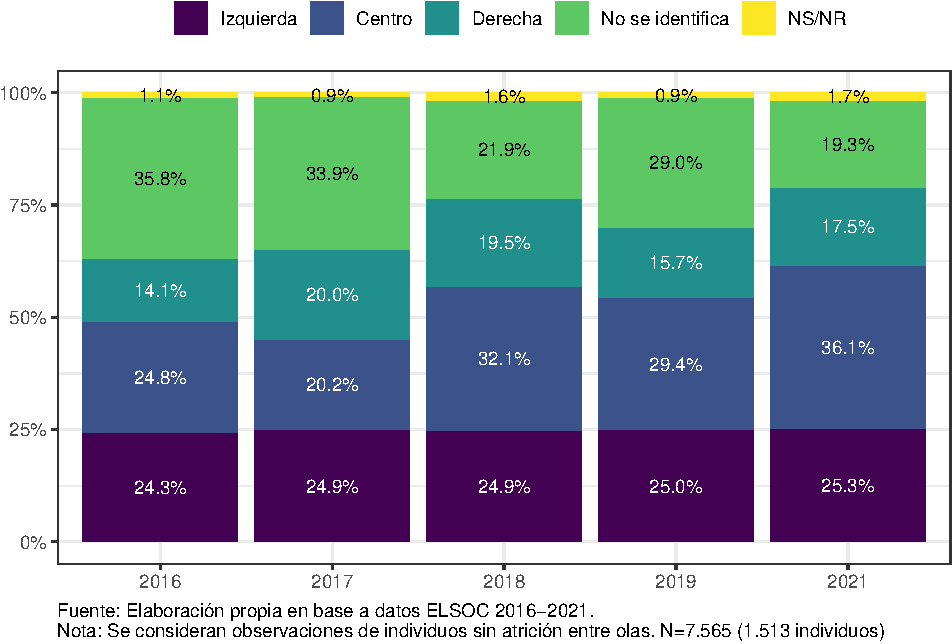
\includegraphics{reporte-elsoc_files/figure-latex/graf-idpolitica-ola-1} 

}

\caption{Identificación política, según ola del estudio}\label{fig:graf-idpolitica-ola}
\end{figure}

Las Figura \ref{fig:graf-alluvial-idpolitica-ola} es un gráfico aluvial que muestra cómo las personas mantienen o cambian sus posiciones ideológicas en cada ola del estudio. Se evidencia como tras los muy estables números agregados de cada año se esconde una proporción importante de personas transitan entre categorías ideológicas, aunque mayoritariamente entre grupos adyacentes.

\begin{figure}

{\centering 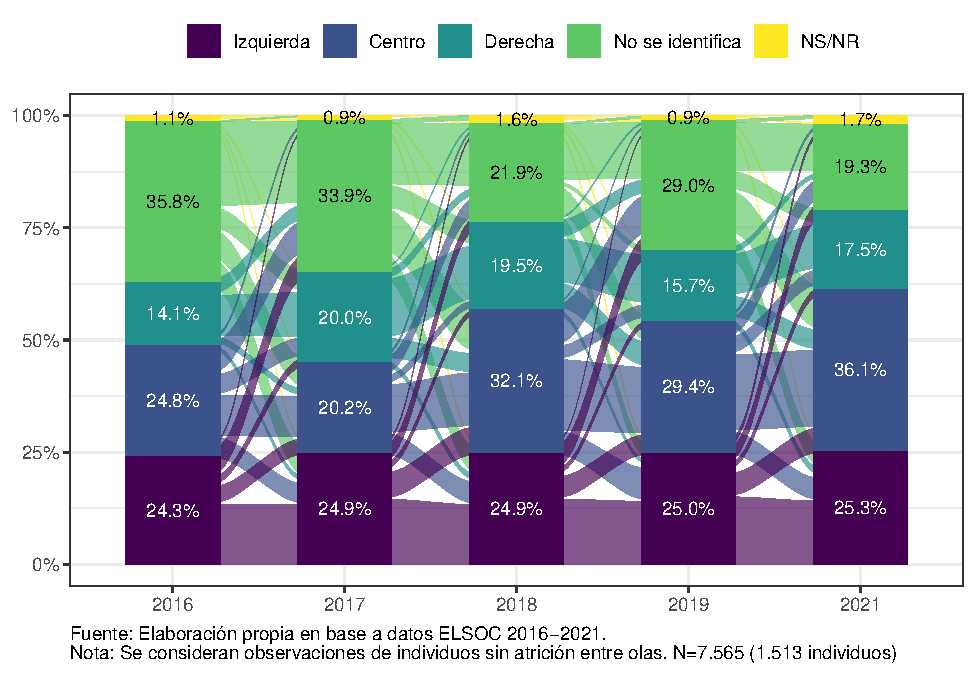
\includegraphics{reporte-elsoc_files/figure-latex/graf-alluvial-idpolitica-ola-1} 

}

\caption{Cambios en identificación política, según ola del estudio}\label{fig:graf-alluvial-idpolitica-ola}
\end{figure}

La Figura \ref{fig:graf-cambios-idpolitica-ola} muestra el porcentaje que en cada ola del estudio respondió otra categoría ideológica que había mencionado el año anterior. Como se puede observar casi la mitad de las personas cambia de posición política consistentemente año a año. Estos patrones hablan a favor de dos segmentos de la población (numéricamente similares); uno con perfiles ideológicos altamente cristalizados y estables, y otro más bien volátil y fluctuante.

\begin{figure}

{\centering 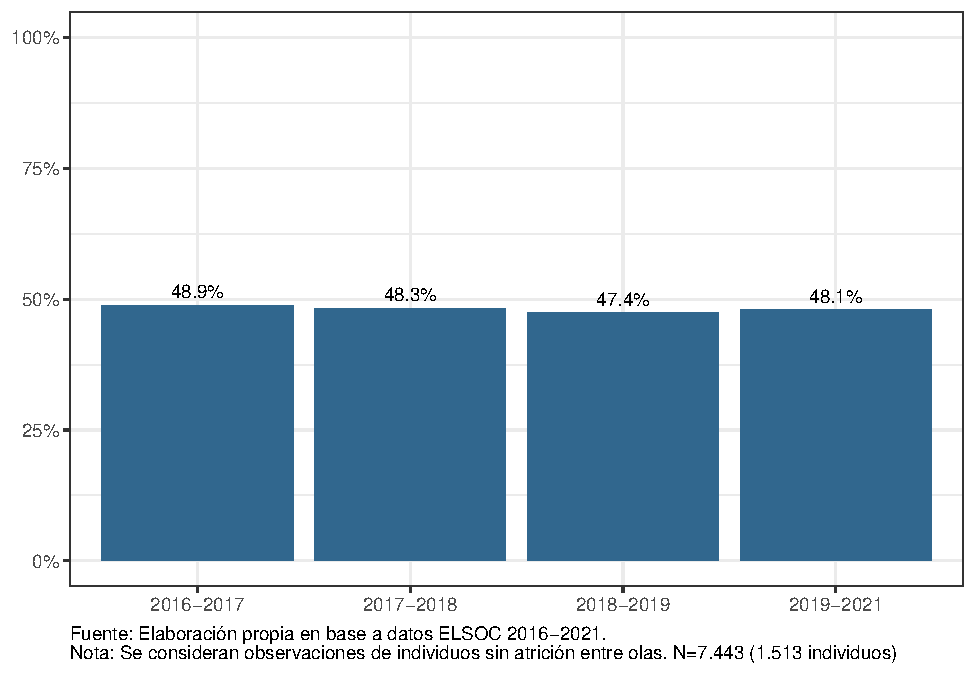
\includegraphics{reporte-elsoc_files/figure-latex/graf-cambios-idpolitica-ola-1} 

}

\caption{Porcentaje que cambia su identificación política entre olas del estudio, según ola}\label{fig:graf-cambios-idpolitica-ola}
\end{figure}

La Figura \ref{fig:graf-cambios-idpol-idpol} muestra el cambio entre posiciones ideológicas entre 2016 y 2021 según la posición mencionada en 2016. Destaca que las personas identificadas con el centro son las más estables, con cerca de un 54\% que se mantuvo en la misma posición. Las personas de izquierda y derecha tienen un comportamiento espejo, donde cerca de un 47\% de cada grupo mantiene su identidad 5 años después de la primera entrevista, mientras que el resto migra mayoritariamente al centro y en una menor proporción a la no identificación. La ausencia de identidad ideológica se asocia a mayor volatilidad, donde sólo un 31\% mantuvo su posición, obteniendo elevada migración al centro (32\%) y la izquierda (21\%). La Figura \ref{fig:graf-cambios-idpolitica-edad} denota que los cambios inter-ola de posición ideológica se concentran mayormente en población jóven (70\% entre 18-29 años), mientras que entre los grupos mayores los niveles de cambio son menores y más similares entre grupos etarios (57\% entre 30-49 años y 50\% entre mayores de 65). Este patrón es enteramente consistente con la hipótesis de los años impresionables según la cual las actitudes de las personas son más inestables durante la adolescencia tardía y la adultez temprana, pero que se solidifican rápidamente y permanecen estables durante el resto del ciclo de vida (Krosnick y Alwin, 1989) .

\begin{figure}

{\centering 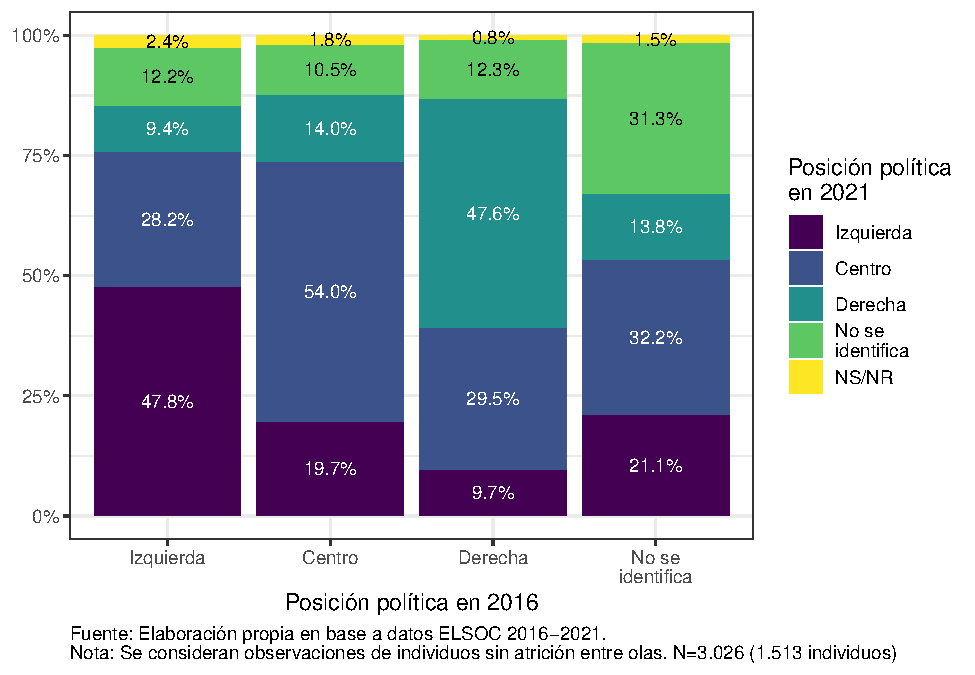
\includegraphics{reporte-elsoc_files/figure-latex/graf-cambios-idpol-idpol-1} 

}

\caption{Posición política en 2021, según posición política en 2016}\label{fig:graf-cambios-idpol-idpol}
\end{figure}

\begin{figure}

{\centering 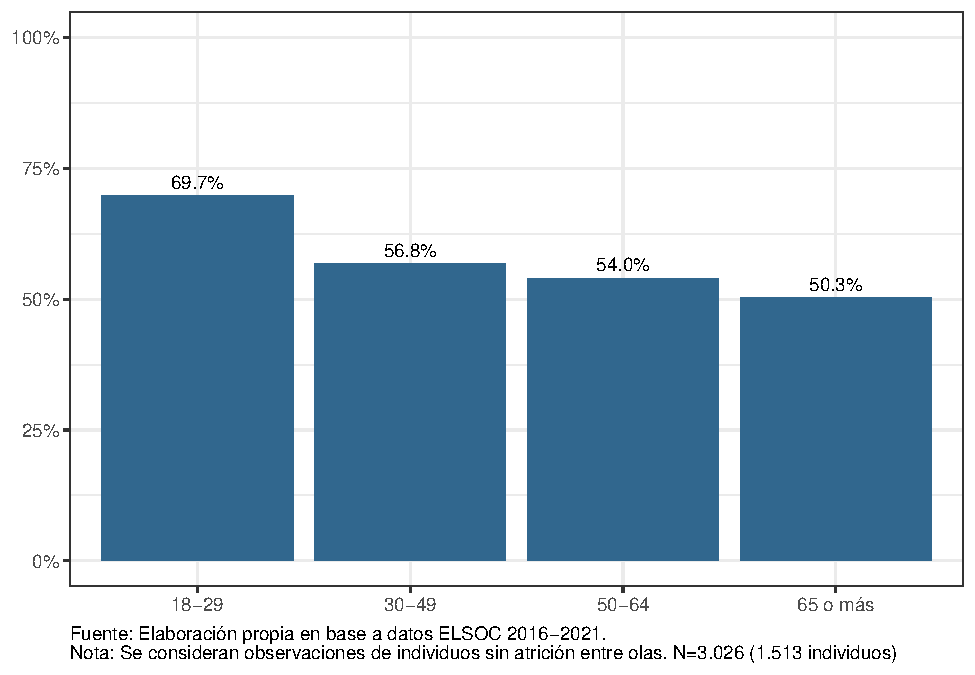
\includegraphics{reporte-elsoc_files/figure-latex/graf-cambios-idpolitica-edad-1} 

}

\caption{Porcentaje que cambia su identificación política entre 2016 y 2021, según grupo etáreo}\label{fig:graf-cambios-idpolitica-edad}
\end{figure}

\hypertarget{interuxe9s-en-la-poluxedtica-y-opiniuxf3n-puxfablica}{%
\section{Interés en la política y opinión pública}\label{interuxe9s-en-la-poluxedtica-y-opiniuxf3n-puxfablica}}

Un antecedente actitudinal fundamental de nivel de participación política de las personas es el nivel de interés general en la política y la frecuencia de discusión sobre temas políticos (Verba, Schlozman y Brady, 1995).

La Figura \ref{fig:graf-interespolitica-ola} muestra que el 2019 se produjo un alza importante en las personas bastante o muy interesadas en la política, pasando de 12,2\% a 21,9\%. Así mismo, la Figura \ref{fig:graf-participciudadana-ola} indica cambios similares en el porcentaje de personas que mencionan hablar de política con familiares (de 16\% a 26\%) o que usan redes sociales para opinar sobre temas políticos (10\% a 20\%). Estas alzas coinciden con las masivas, y en ocasiones altamente disruptivas, marchas ocurridas en el marco del llamado estallido social (la medición del 2019 se inició el 20 de noviembre). En contraste, el incremento en los niveles de politización observados entre 2018 y 2019 se revierten en buena medida en la última ola del estudio, donde el nivel de interés en política cae a un 15,2\%, el hablar de política con familiares a un 21\%, y el uso de redes sociales para opinar sobre temas políticos a un 14.5\%.

\begin{figure}

{\centering 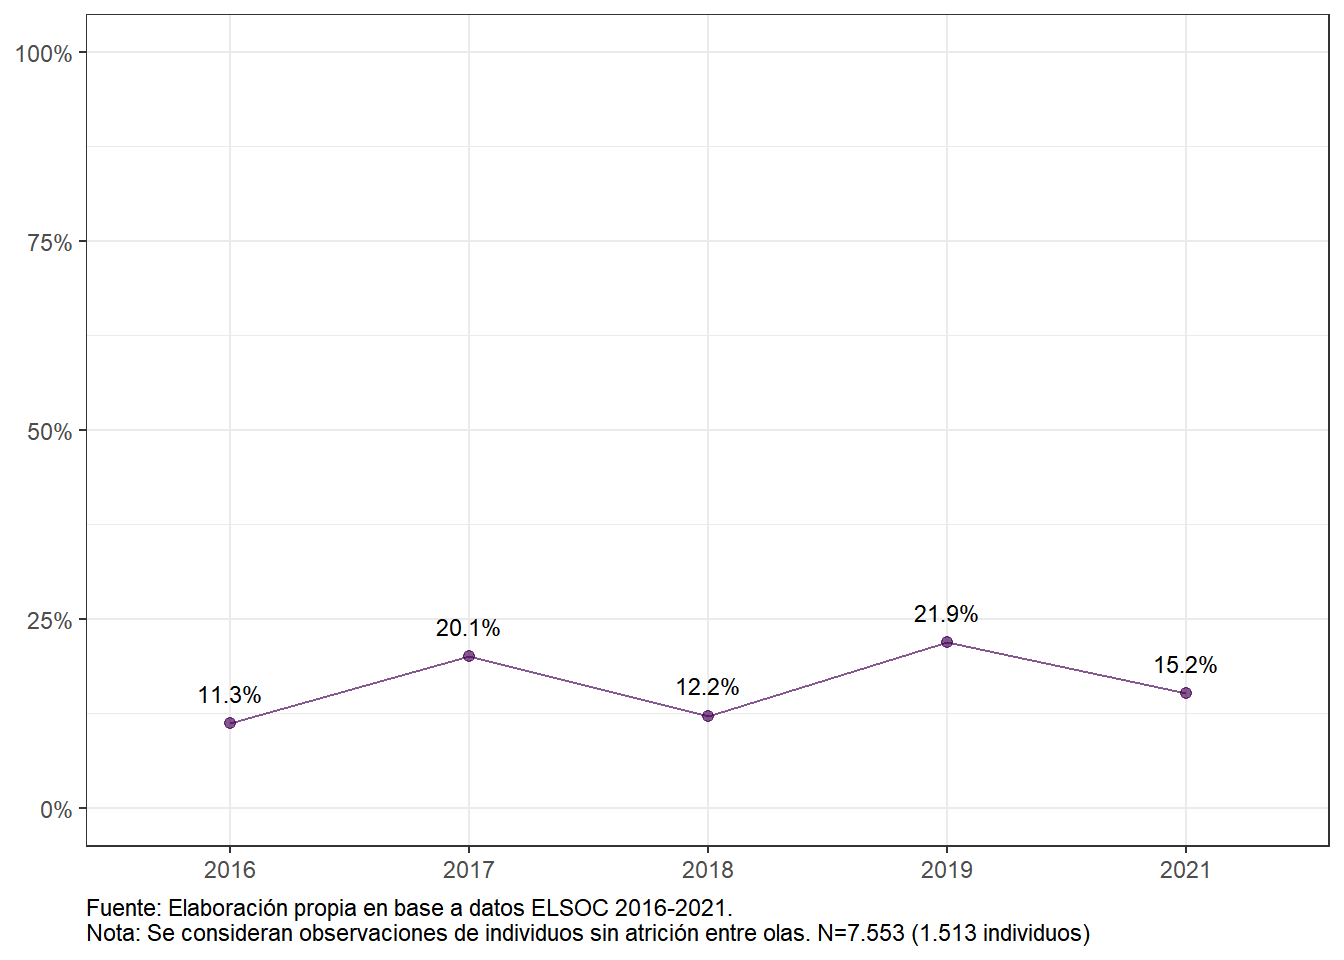
\includegraphics{reporte-elsoc_files/figure-latex/graf-interespolitica-ola-1} 

}

\caption{Porcentaje Bastante o Muy interesado en política, según ola del estudio}\label{fig:graf-interespolitica-ola}
\end{figure}

\begin{figure}

{\centering 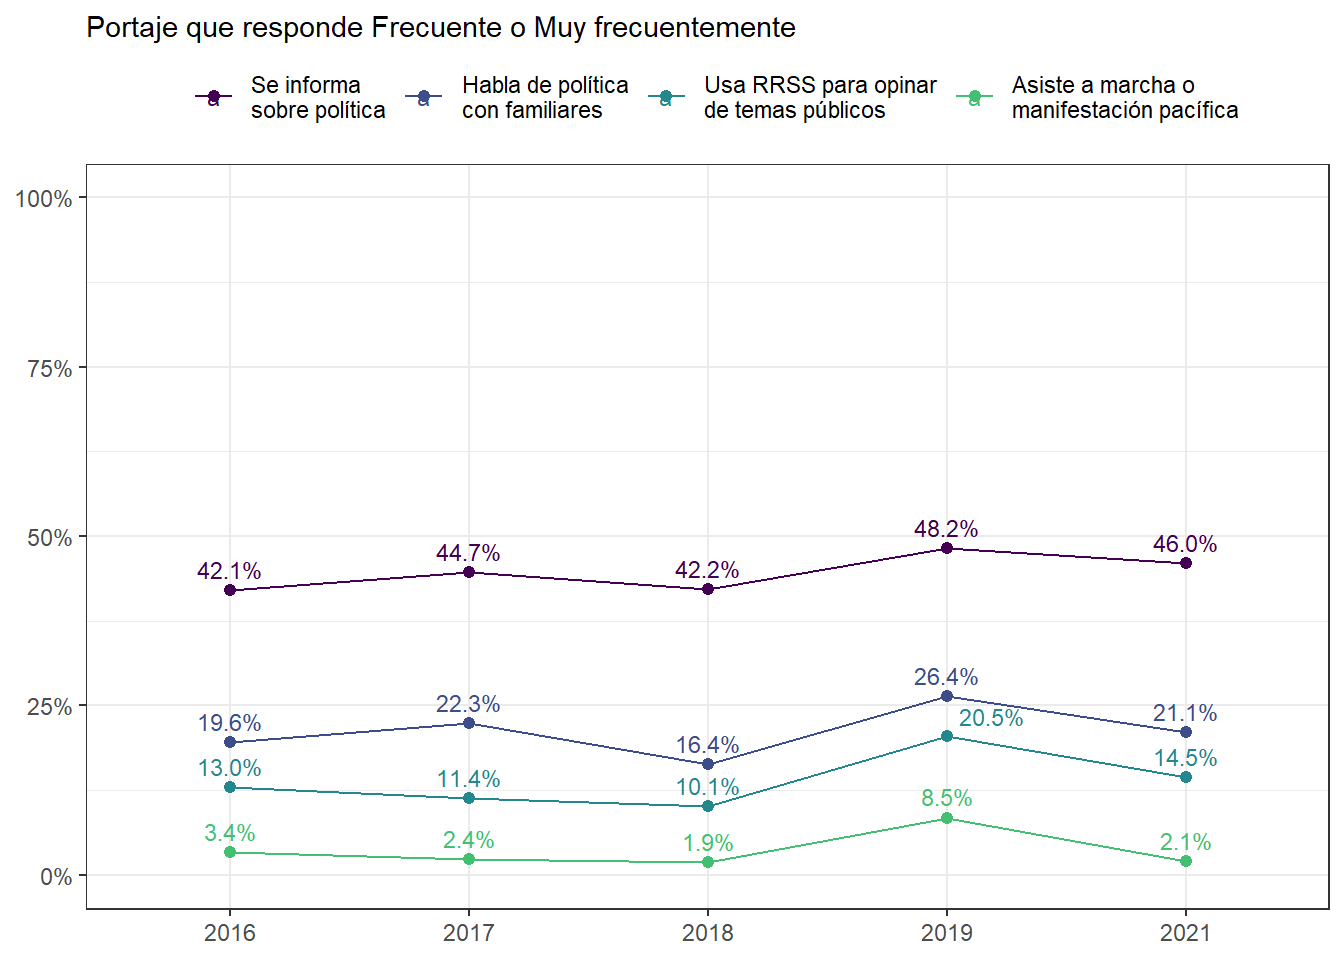
\includegraphics{reporte-elsoc_files/figure-latex/graf-participciudadana-ola-1} 

}

\caption{Participación ciudadana, según ola del estudio}\label{fig:graf-participciudadana-ola}
\end{figure}

La Figura \ref{fig:graf-idpolitica-interespolitica} muestra una fuerte asociación estadística entre interés en política y preferencias ideológicas en el año 2021. La proporción de personas de izquierda crece en categorías de mayor interés, mientras que los individuos de derecha alcanzan proporciones similares sin importar el nivel de interés político. Los sujetos de centro se concentran en mayor medida en niveles de interés bajos, mientras que los sujetos que no se identifican tienden a coincidir con ausencia de interés en la política.

\begin{figure}

{\centering 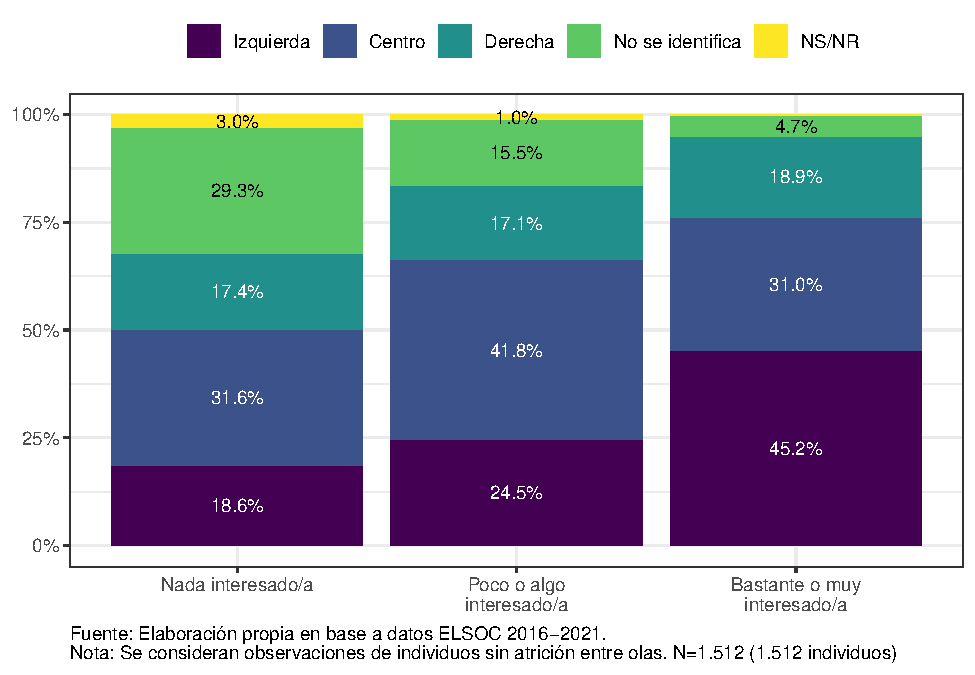
\includegraphics{reporte-elsoc_files/figure-latex/graf-idpolitica-interespolitica-1} 

}

\caption{Identificación política, según grado de interes en la política (2021)}\label{fig:graf-idpolitica-interespolitica}
\end{figure}

ELSOC también ha registrado durante múltiples años la opinión de las personas encuestadas respecto a diversos temas de discusión pública. Aquí pueden volver a verse patrones de cambio y estabilidad entre los años 2019 y 2021. La Figura \ref{fig:graf-temaspublicos-idpolitica} muestra, por un lado, que todos los grupos ideológicos han mantenido su posición frente al tema del aborto libre, pero por otra parte, se observa un incrementado acentuado, que fluctua entre los 12 y 17 puntos porcentuales, en el nivel de acuerdo con tomar medidas más drásticas para evitar mayor inmigración. Las alzas se pueden incluso notar en grupos menos proclives a estar de acuerdo con mayores restricciones como las personas que se identifican con la izquierda. En materia de pensiones, las personas de izquierda y centro han mantenido sus posiciones similares, mientras que las de derecha y que no se identifican han incrementado su acuerdo con que las personas deben ser responsables de su propia pensión, cuestión que puede deberse a la mediatización de los retiros de las AFP como derecho de propiedad individual sobre los fondos de pensiones.

\begin{figure}

{\centering 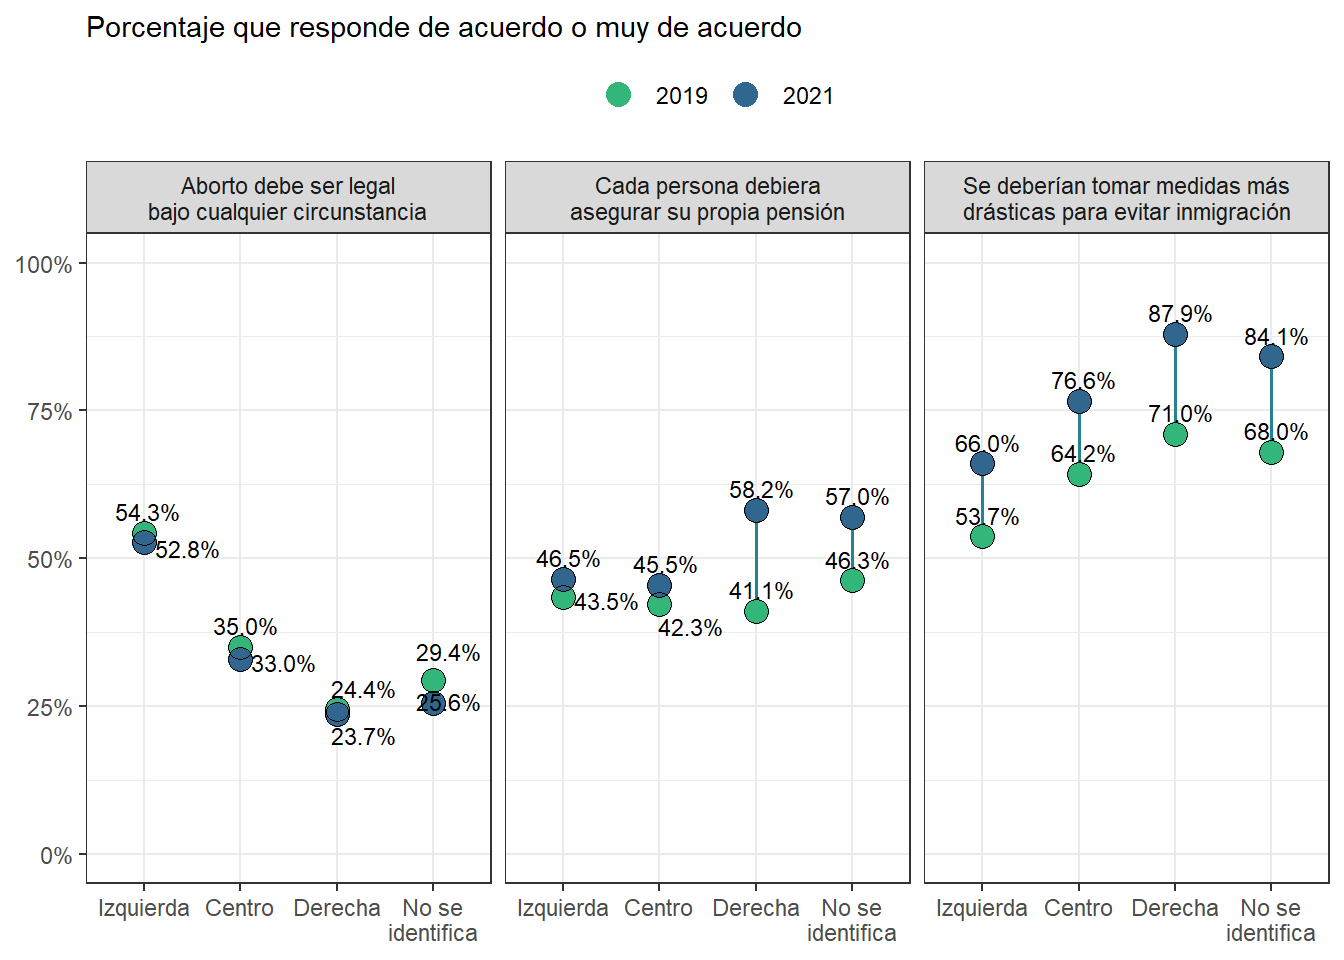
\includegraphics{reporte-elsoc_files/figure-latex/graf-temaspublicos-idpolitica-1} 

}

\caption{Acuerdo con temas de discusión pública, según posición política (2019-2021)}\label{fig:graf-temaspublicos-idpolitica}
\end{figure}

\hypertarget{anuxe1lisis-de-clases-latentes-participaciuxf3n-poluxedtica}{%
\section{Análisis de Clases Latentes: Participación política}\label{anuxe1lisis-de-clases-latentes-participaciuxf3n-poluxedtica}}

El proceso de cambio constitucional, las recientes elecciones presidenciales y el estallido social han implicado transformaciones en materia de participación política en el país. El plebiscito superó por primera vez el 50\% de participación desde la instauración del voto voluntario e inscripción automática, mientras que la segunda vuelta presidencial incorporó a cerca de 1.300.000 votantes más que la misma elección de 2017. Asimismo, el estallido social supuso un incremento nunca antes visto de eventos de protesta (Observatorio de Conflictos, 2020). Ante este panorama, cabe preguntarse cómo es la estructura longitudinal de participación política de los chilenos y chilenas, tanto en el ámbito electoral como en manifestaciones.

\hypertarget{perfiles-de-participaciuxf3n-aproximaciuxf3n-empuxedrica}{%
\subsection*{Perfiles de participación: aproximación empírica}\label{perfiles-de-participaciuxf3n-aproximaciuxf3n-empuxedrica}}
\addcontentsline{toc}{subsection}{Perfiles de participación: aproximación empírica}

Con el objetivo de determinar patrones de participación política en el tiempo, se efectuó un análisis de clases latentes que permitió categorizar a los individuos según sus patrones de participación en el plebiscito constituyente, las elecciones presidenciales de 2013 y 2017, y en eventos de protesta (consideramos si declararon participar -a veces, frecuentemente o muy frecuentemente- en marchas o manifestaciones pacíficas en cada una de las cinco olas del estudio). El análisis arrojó cinco categorías de participación política: (1) Reactivos, (2) Desafectados, (3) Politizados, (4) Institucionales y (5) Hiper-politizados.

\hypertarget{perfiles-de-participaciuxf3n-principales-resultados}{%
\subsection*{Perfiles de participación: principales resultados}\label{perfiles-de-participaciuxf3n-principales-resultados}}
\addcontentsline{toc}{subsection}{Perfiles de participación: principales resultados}

La Figura \ref{fig:tip-participacion5} muestra los perfiles de participación identificados y su caracterización según las variables que compusieron el análisis de clases latentes. El grupo más numeroso, con un 47,2\% de los individuos, corresponde a los Institucionales, que participan reiteradamente de procesos electorales y son inactivos en protestas. La participación electoral de estos individuos se acrecentó en las elecciones de 2017, aunque se redujo en el plebiscito de 2020.

Consistente con el diagnóstico de un elevado nivel de desconfianza política en la sociedad chilena, un 28,9\% compone el grupo de Desafectados. Estos se caracterizan por sus virtualmente nulos niveles de participación política, ya sea convencional (votar) o no convencional (participar en marchas). No obstante, se observan niveles de participación más elevados en las elecciones de 2013 y el plebiscito, aunque muy distantes de los promedios nacionales.

Un 17,3\% compone el grupo de Politizados, individuos con -relativamente hablando- elevados niveles de participación electoral y participación en protestas. Los integrantes de este grupo fueron particularmente activos en las movilizaciones de 2019, año en que su participación no convencional triplicó la de años anteriores.

Un 3,9\% son los Reactivos, quienes suelen tener bajos niveles de participación electoral y en manifestaciones, aunque se involucraron sustantivamente en el plebiscito de 2020 y en las movilizaciones de 2019. Así, estos individuos requieren de eventos de participación ampliamente mediatizados y debatidos en la opinión pública para involucrarse en la vida cívica.

Finalmente, están los llamados Hiper-politizados, que se caracterizan por ser un grupo muy pequeño de la muestra (2,7\%), pero que son inusualmente activos en la expresión de su voz ya sea en eventos electorales o en manifestaciones. Su participación se redujo levemente en 2019 y 2021, aunque también incrementó en el plebiscito 2020.

En suma, los resultados indican que los grupos que menos expresan su voz política son también los más grandes en términos numéricos (Desafectados e Institucionales suman el 76\% de la muestra), al tiempo que el grupo, por lejos, más activo es el más pequeño (Hiper politizados).

\begin{figure}

{\centering 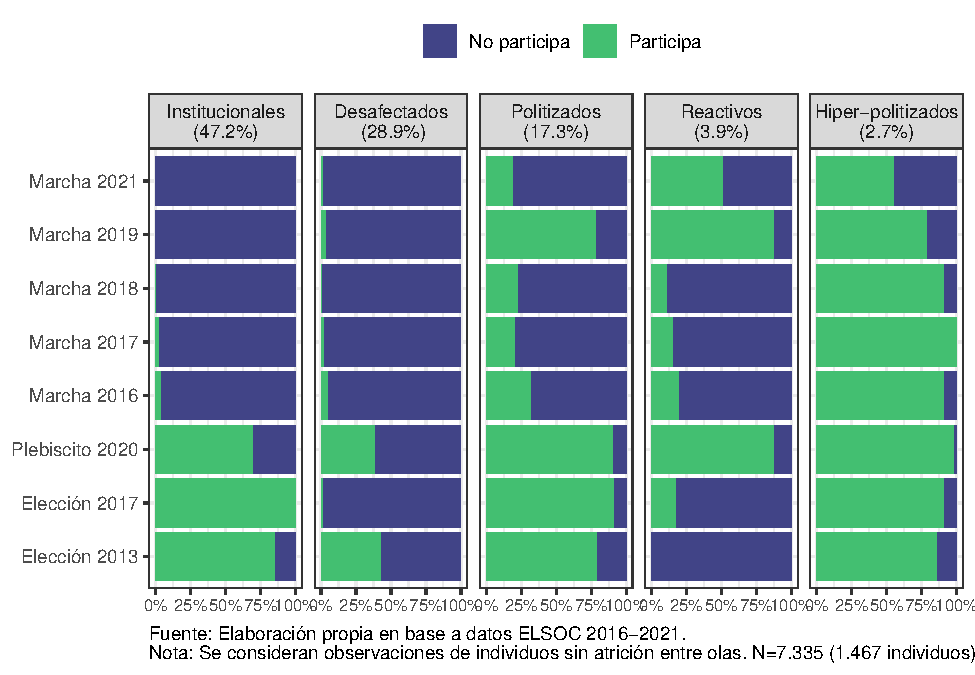
\includegraphics{reporte-elsoc_files/figure-latex/tip-participacion5-1} 

}

\caption{Perfiles de participación política: 5 clases}\label{fig:tip-participacion5}
\end{figure}

\hypertarget{caracterizaciuxf3n-de-perfiles-de-participaciuxf3n}{%
\subsection*{Caracterización de perfiles de participación}\label{caracterizaciuxf3n-de-perfiles-de-participaciuxf3n}}
\addcontentsline{toc}{subsection}{Caracterización de perfiles de participación}

La Figura \ref{fig:tipos-posicion-politica2} muestra cómo se distribuyen estos grupos según posiciones ideológicas. Destacan los Hiper-politizados por su elevado nivel de homogeneidad ideológica con una fuerte concentración de individuos auto posicionados como de izquierda (65,7\%). Aunque en forma más matizada, las personas de izquierda también se encuentran concentrados entre los Politizados con un 40\%, seguidos por las personas de centro con un 35,9\%. En contraste, los Desafectados están mayoritariamente compuestos por individuos de centro (35,3\%) o sin identificación política (32\%). El grupo con mayor presencia de derecha es el de Institucionales (21,8\%), aunque tienen una proporción similar de individuos de izquierda (20,8\%) y también cuentan con una fuerte presencia de encuestados que se identifican con el centro político (38,8\%). El grupo de los Reactivos es el que concentra un mayor porcentaje de sujetos de centro (43,2\%), seguidos de un 29,2\% de individuos de izquierda.

\begin{figure}

{\centering 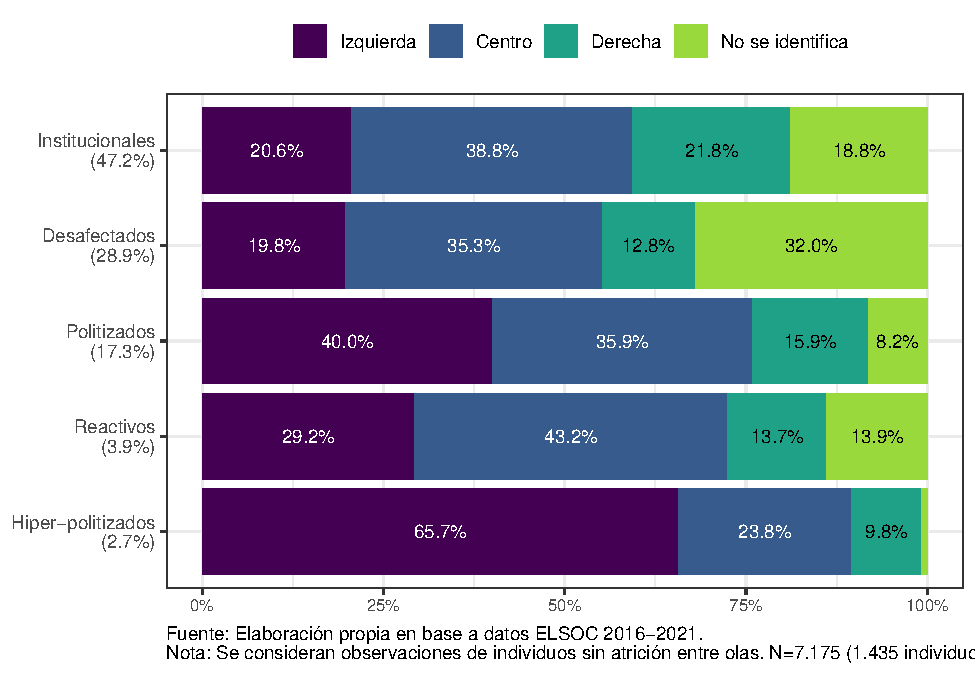
\includegraphics{reporte-elsoc_files/figure-latex/tipos-posicion-politica2-1} 

}

\caption{Posición política según perfil de participación}\label{fig:tipos-posicion-politica2}
\end{figure}

La Figura \ref{fig:tipos-sexo2} muestra que el grupo de Politizados es el único en que predominan los hombres (59,9\%), mientras que en los Hiper-politizados y Reactivos son marcadamente mayoritarias las mujeres, con un 68,9\% y 56,9\% respectivamente. Los Institucionales y Desafectados parecen tener una distribución por sexo más equilibrada con alrededor de un 54\% de mujeres y 46\% de hombres. La Figura \ref{fig:tipos-edad2} indica marcadas variaciones en términos de edad. Los Reactivos, Desafectados e Hiper-politizados son los grupos con mayor concentración de adultos jóvenes, con un 57,6\%, 55,9\% y 51,8\% respectivamente. Se presentan también altos porcentajes de población juvenil en los Reactivos (33,5\%) y Politizados (23,4\%). Los Institucionales, en cambio, obtienen la más alta proporción de adultos mayores y mediana edad, con un 26,3\% y 40,6\%, respectivamente.

\begin{figure}

{\centering 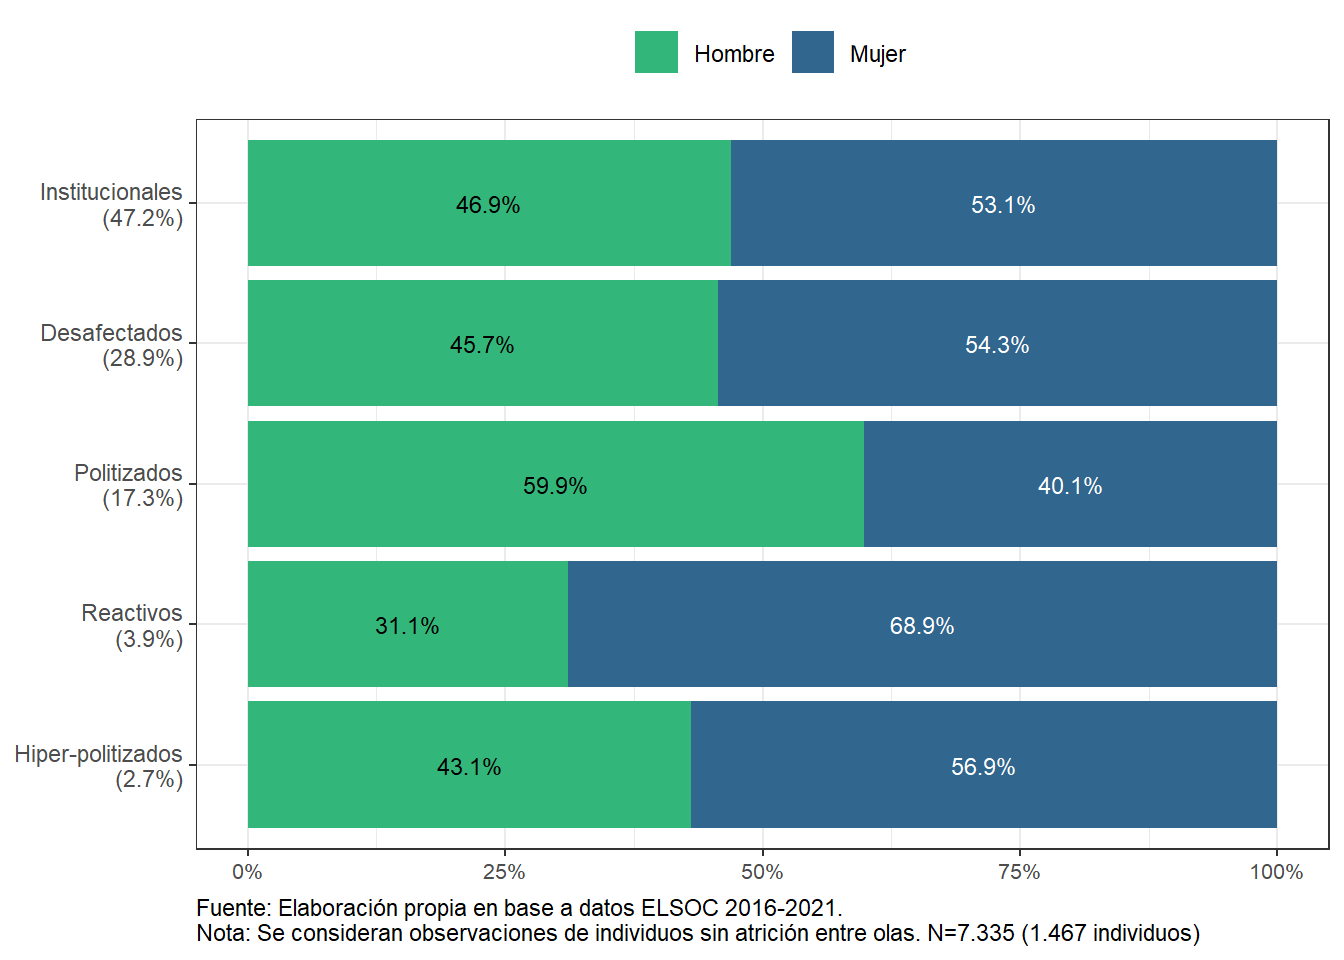
\includegraphics{reporte-elsoc_files/figure-latex/tipos-sexo2-1} 

}

\caption{Sexo según perfil de participación}\label{fig:tipos-sexo2}
\end{figure}

\begin{figure}

{\centering 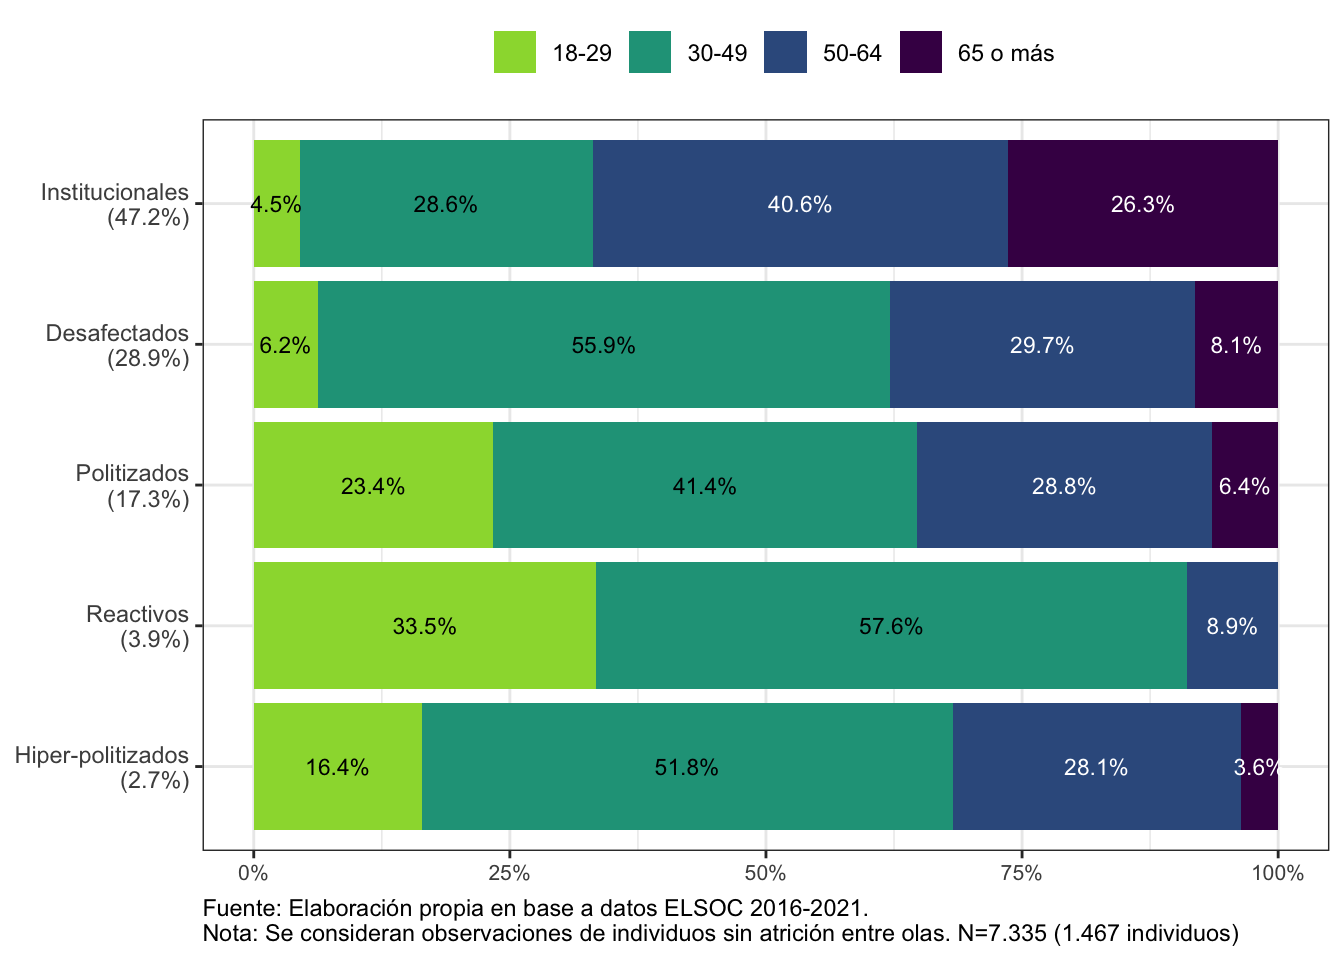
\includegraphics{reporte-elsoc_files/figure-latex/tipos-edad2-1} 

}

\caption{Edad según perfil de participación}\label{fig:tipos-edad2}
\end{figure}

La Figura \ref{fig:tipos-interes2} indica que los grupos con menor interés en la política son los Desafectados e Institucionales, con un 79,1\% y 70,1\% de personas con nada o poco interés. A ello le siguen los Politizados y Reactivos, con un 45,1\% y 44,4\%, respectivamente. El grupo de Hiper-politizados es el que alcanza mayores niveles de interés, con un 62,8\% de individuos muy o bastante interesados, seguido de los Reactivos y Politizados con un 27,3\% y 25,6\%. Este patrón resulta del todo relevante ya que confirma que en Chile las personas más politizadas expresan sus demandas y preocupaciones por los canales no institucionales, al tiempo que los menos politizados abiertamente no participan de ninguna instancia o si lo hacen emplean los canales formales.

\begin{figure}

{\centering 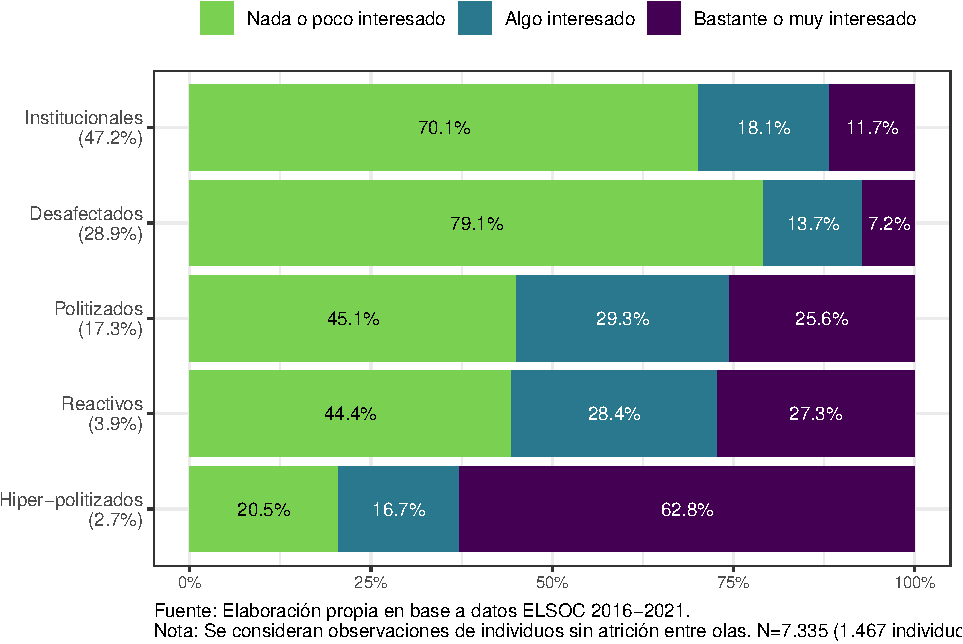
\includegraphics{reporte-elsoc_files/figure-latex/tipos-interes2-1} 

}

\caption{Interés en la política según perfil de participación}\label{fig:tipos-interes2}
\end{figure}

La Figura \ref{fig:tipos-satisfaccion2} muestra una alta insatisfacción con la democracia de parte de todos los grupos, aunque esta es aún más pronunciada en el grupo de los Hiper-politizados (83,6\%) y Reactivos (79\%). Si sumamos los porcentajes de personas altamente satisfechas y algo satisfechas, los niveles de satisfacción con la democracia son más altos entre los Politizados, Desafectados e Institucionales. Es decir, hay una marcada distancia de toda forma de acción política y la focalización en canales institucionales parecen ser indicativos de mayores niveles de satisfacción política.

\begin{figure}

{\centering 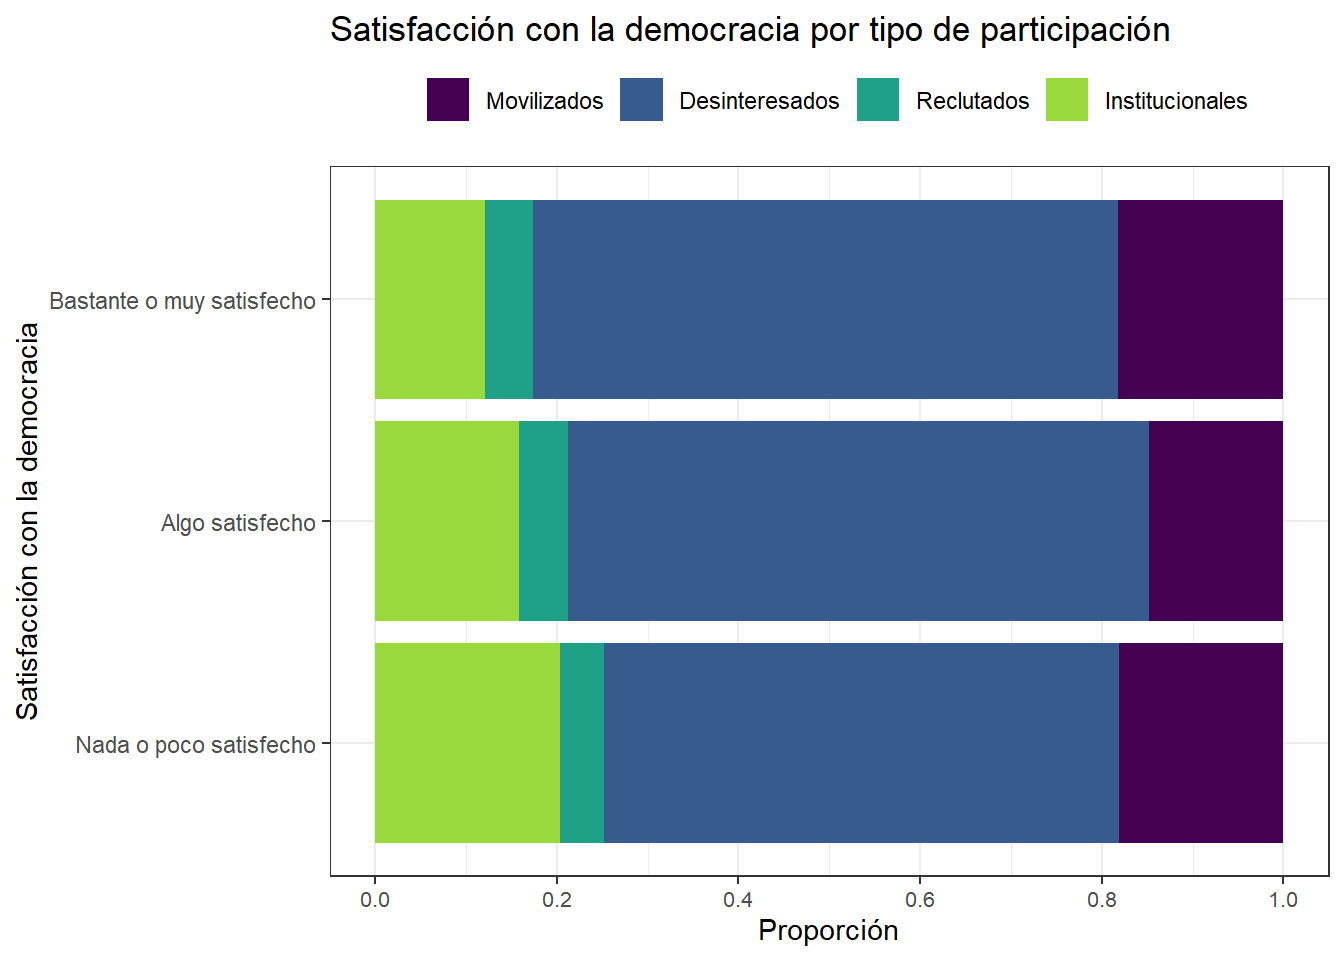
\includegraphics{reporte-elsoc_files/figure-latex/tipos-satisfaccion2-1} 

}

\caption{Satisfacción con la democracia según perfil de participación}\label{fig:tipos-satisfaccion2}
\end{figure}

La Figura \ref{fig:tipos-legitimidad2} muestra que los Hiper-politizados y Politizados tienen una mayor preferencia por la democracia como régimen de gobierno, con un 88,1\% y 81,3\% respectivamente, versus sólo un 49,8\%, 49,2\% y 47,1\% de apoyo democrático entre los Reactivos, Institucionales y Desafectados. Esto implica, no sin bastante ironía, que el grupo que más vota en elecciones políticas nacionales es, junto al que jamás participa políticamente, el que menos explícitamente apoya la democracia como régimen político.

\begin{figure}

{\centering 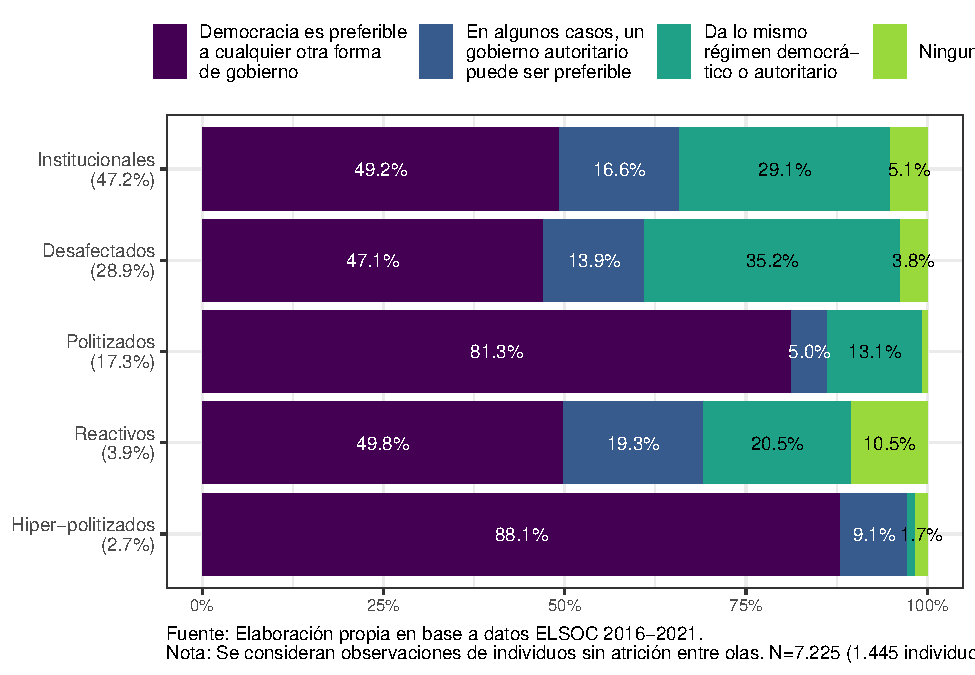
\includegraphics{reporte-elsoc_files/figure-latex/tipos-legitimidad2-1} 

}

\caption{Legitimidad democrática según perfil de participación}\label{fig:tipos-legitimidad2}
\end{figure}

Respecto al actual proceso constituyente, la Figura \ref{fig:tipos-optimismo2} muestra los niveles de optimismo constitucional. Se observan los mayores niveles de optimismo entre Hiper-politizados y Politizados, con más de un 70\% de optimismo en ambos grupos. Los Reactivos están justo por debajo con un 69,3\%, mientras que los Institucionales y Desafectados alcanzan un optimismo del 60,3\% y 56\%. Esto implica que entre todos los grupos prevalece una sensación positiva acerca del proceso constitucional, pese a existir diferencias inter-grupales relevantes en otras materias.

\begin{figure}

{\centering 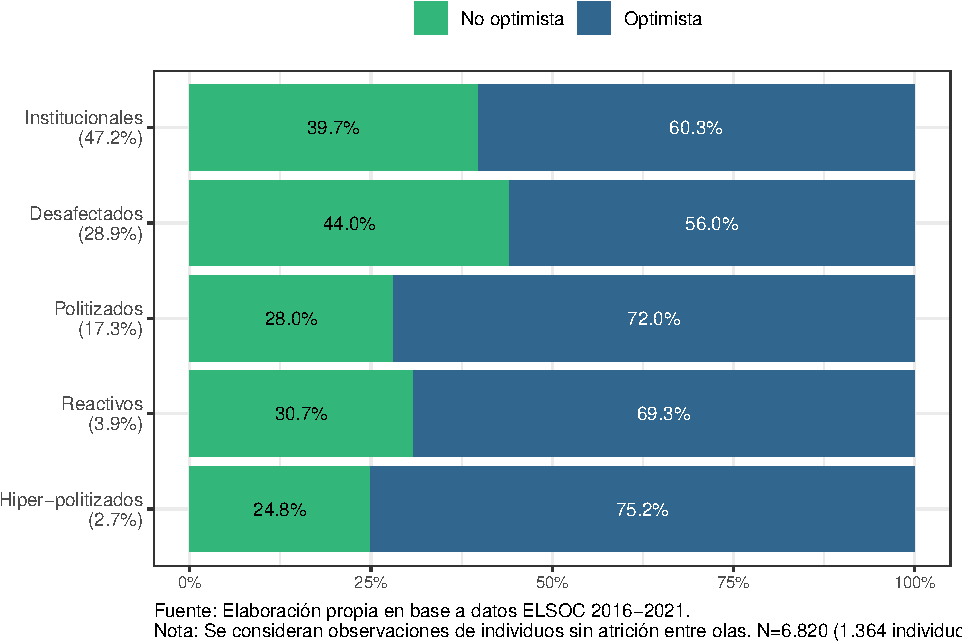
\includegraphics{reporte-elsoc_files/figure-latex/tipos-optimismo2-1} 

}

\caption{Optimismo constitucional según perfil de participación}\label{fig:tipos-optimismo2}
\end{figure}

\hypertarget{ciclo-de-movilizaciuxf3n-poluxedtica-y-estallido-social}{%
\section{Ciclo de movilización política y estallido social}\label{ciclo-de-movilizaciuxf3n-poluxedtica-y-estallido-social}}

Desde hace varios años en Chile se han desarrollado múltiples movimientos sociales, algunos de los cuales corresponden a movimientos progresistas, orientados a promover cambio social (por ejemplo, el movimiento Estudiantil, de pensiones, ambientalista) y otros a movimientos más conservadores (por ejemplo, el movimiento pro-vida o antiaborto o movimie to antidelicuencia). Proveyendo una lista de movimientos que han alcanzado visibilidad en Chile, se les ha consultado a los/as chilenos/as por los movimientos que más valoran. Tal como se puede apreciar en la Figura \ref{fig:graf-movsocial}, para 7 movimientos se ha observado un aumento gradual en los niveles de valoración, (5 progresistas y 2 conversadores). Sin embargo, llama la atención la disminución sustantiva que alcanzó la valoración del estallido social pasando desde un 22,8 \% a un 15,7 \% en el 2021. En su conjunto la valoración da cuenta del nivel de apoyo que tienen estos movimientos sociales.

\begin{figure}

{\centering 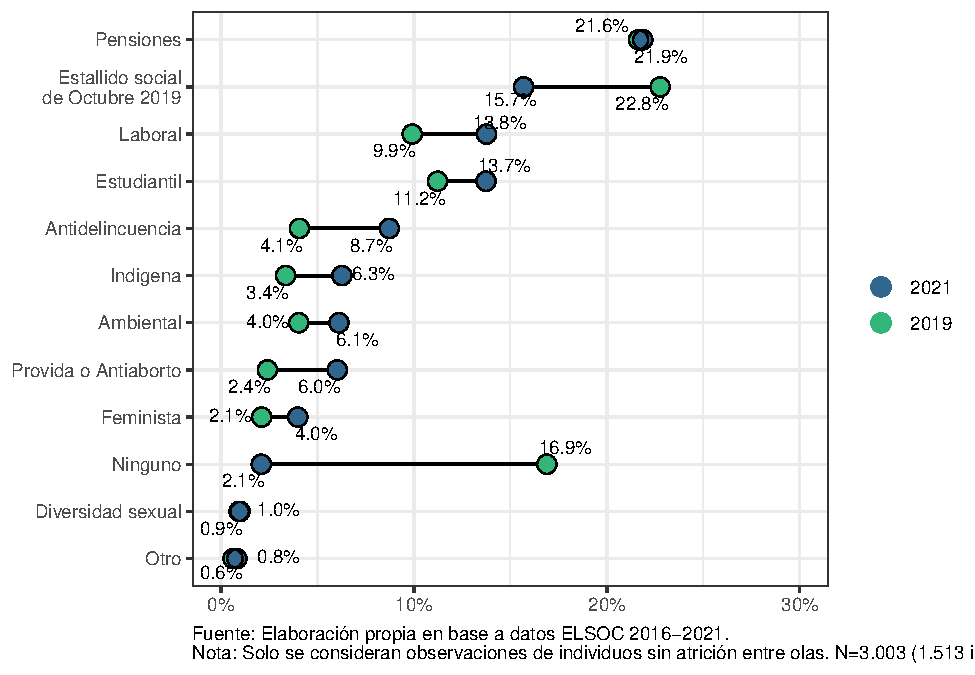
\includegraphics{reporte-elsoc_files/figure-latex/graf-movsocial-1} 

}

\caption{¿Cuál de los siguientes movimientos sociales más valora? (2019-2021)}\label{fig:graf-movsocial}
\end{figure}

Al analizar cómo ha evolucionado la valoración de los movimientos progresistas y conservadores a lo largo de los años (ver Figura \ref{fig:graf-movsociales-movsocial-olas}), se puede constatar un aumento sustantivo de la valoración de los movimientos progresistas que alcanzan un nivel muy alto el año del estallido social (2019) y el año en que se llevó a cabo el plebiscito para la convención constituyente (2021). Esta alta valoración de los movimientos progresistas revela en parte el nivel de politización que alcanzó la población, particularmente durante los dos últimos años al valorar aquellos movimientos que se orientan particularmente al cambio social. Un patrón opuesto se observa en el caso de los movimientos conservadores donde se constata una caída gradual a lo largo de los años de su valoración, aunque se registra una importante recuperación entre el 2019 y 2021 donde pasa de un 6.5\% a 14.7\%.

\begin{figure}

{\centering 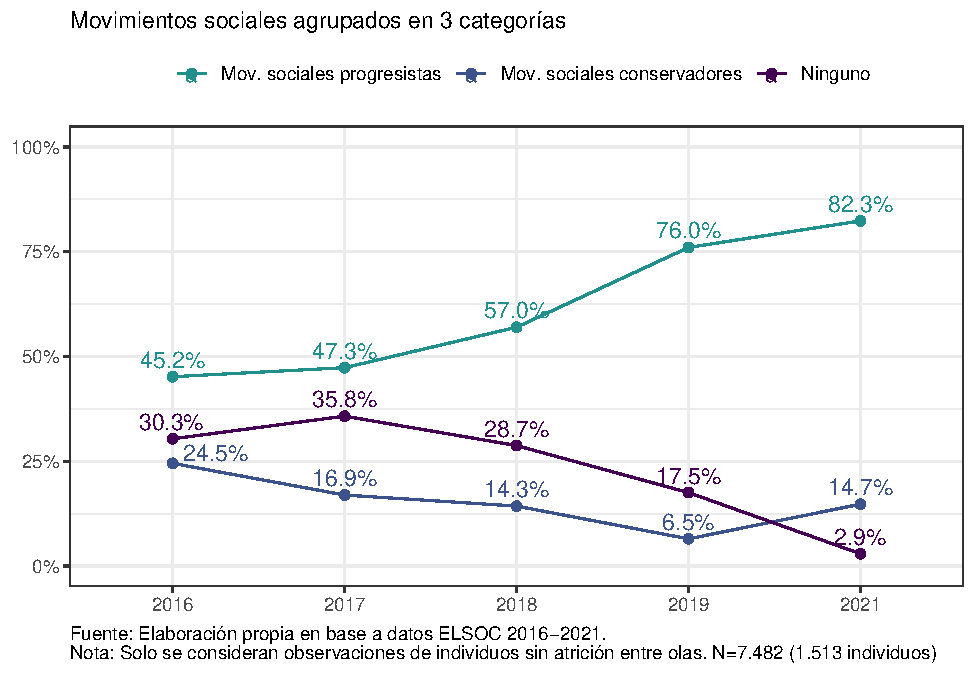
\includegraphics{reporte-elsoc_files/figure-latex/graf-movsociales-movsocial-olas-1} 

}

\caption{Movimiento social que más valora, Según ola}\label{fig:graf-movsociales-movsocial-olas}
\end{figure}

Cuando analizamos la participación política según el movimiento social más valorado a lo largo del tiempo, verificamos que los/as chilenos/as reportan bajos niveles de participación entre los años 2016 y 2018, puesto que solo 5.2\% y 4.0\% respectivamente reportan participar ``frecuentemente o muy frecuentemente'' en el movimiento social que más valoran. Ya el año 2019, el año en que ocurre el estallido social, la participación sube considerablemente alcanzando un 11.2\% de personas que participan ``frecuentemente o muy frecuentemente.'' Si bien es cierto durante el 2021 se observa una caída respecto del año anterior, los niveles de participación fluctúan en torno a un 10.1\%. Estos resultados apuntan a que, por lo general, la participación regular en movimientos sociales es baja en Chile pero que, en el contexto del Estallido Social y el año siguiente, los niveles de participación suben y se mantienen relativamente elevados en comparación con años anteriores.

\begin{figure}

{\centering 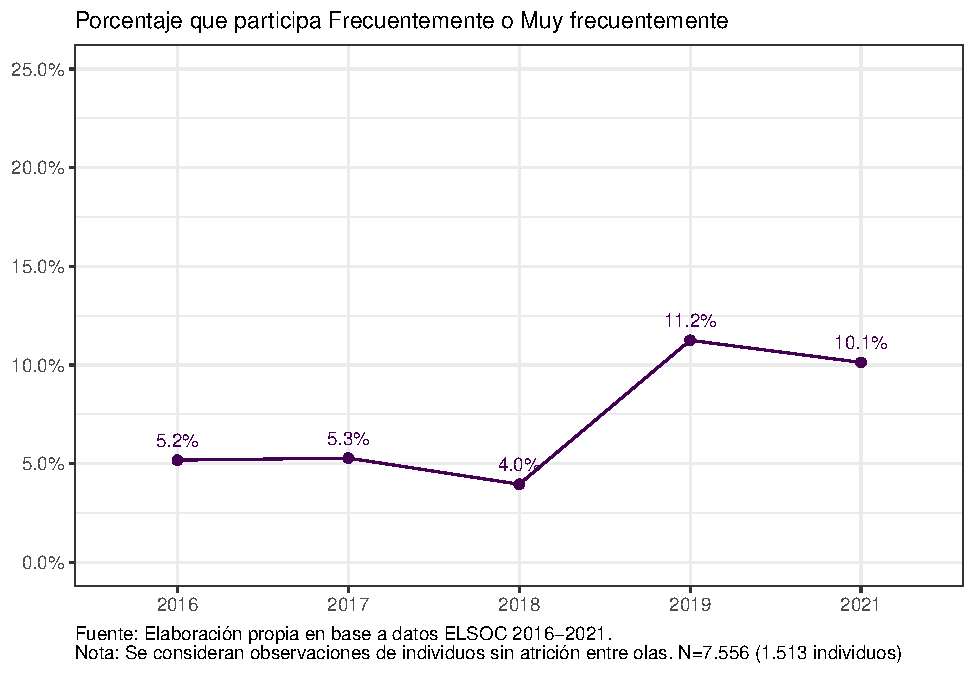
\includegraphics{reporte-elsoc_files/figure-latex/graf-participmovsocial-olas-1} 

}

\caption{Participación en movimientos sociales valorados, según ola}\label{fig:graf-participmovsocial-olas}
\end{figure}

Cuando nos enfocamos en la evolución de la participación en movimientos progresistas y conservadores a lo largo de los años, se constata un aumento de la participación en los movimientos progresistas durante 2019, año en que 14.5\% de los/as chilenos/as reportan participar ``frecuentemente o muy frecuentemente'' en este tipo de movimientos sociales. No obstante, la participación regular en movimientos progresistas disminuye un poco el año de 2021 (con 11.8\% de personas reportando participar ``frecuentemente o muy frecuentemente'').

Por otro lado, la participación en movimientos sociales conservadores, tiene un peak el año de 2017, con 5\% de las personas reportando participar ``frecuentemente o muy frecuentemente,'' valor que decae a 1.3\% durante el Estallido Social (2019), subiendo de nuevo a 3.1\% durante 2021. Finalmente, el porcentaje de personas que reporta no participar de ningún movimiento social fluctúa entre el 2\% y el 1.4\% entre 2016 y 2021.

En su conjunto, estos resultados revelan mayores niveles de movilización social relacionados con temáticas y demandas progresistas a lo largo del tiempo, en comparación con la movilización en torno a movimientos más conservadores.

\begin{figure}

{\centering 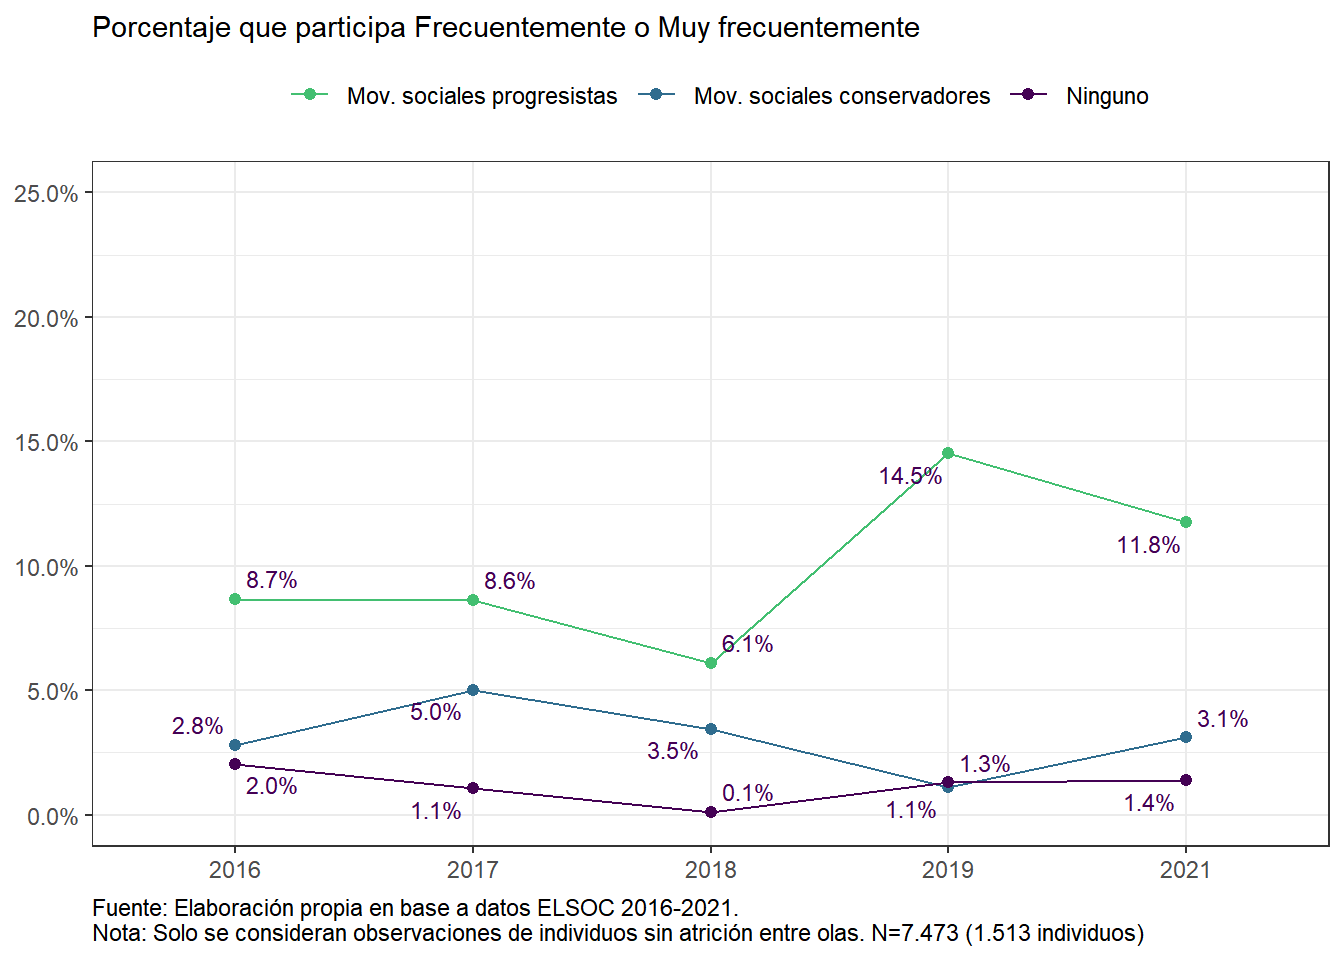
\includegraphics{reporte-elsoc_files/figure-latex/graf-participmovsociales2-ola-1} 

}

\caption{Participación en tipos de movimientos sociales, según ola}\label{fig:graf-participmovsociales2-ola}
\end{figure}

\hypertarget{justificaciuxf3n-de-la-violencia}{%
\section{Justificación de la Violencia}\label{justificaciuxf3n-de-la-violencia}}

La justificación de la violencia por parte de diferentes grupos siempre ha existido en las sociedades. En este sentido, para algunas personas, parece razonable la utilización de violencia para imponer demandas (violencia para el cambio social) mientras, para otras, la violencia policial o ciudadana se justifica si tiene como fin mantener el orden y seguridad en un contexto de alta efervescencia social (violencia para el control social). No obstante, el uso de la violencia, más allá de su propósito, trae consigo el riesgo de aumentar ciclos de violencia, generando una potencial escalada de hechos violentos que ponen en riesgo la convivencia y la seguridad de la ciudadanía y las fuerzas del orden. En Chile, desde el Estallido Social, se han visto distintos tipos de actos violentos y por ende es necesario entender cómo se configuran los cambios en la justificación de la violencia por parte de las fuerzas de orden y de la sociedad civil.

En particular, la violencia para el control social se refiere a actos de agresión física que tienen como finalidad mantener o restablecer el orden social imperante y se puede distinguir entre violencia llevada a cabo de manera privada por ciudadanos (linchamientos) y violencia institucional (violencia de Carabineros).

En ELSOC, analizamos la evolución de la justificación de dos tipos de violencia que buscan el control social: la violencia a manos de ciudadanos y la violencia policial.

Como se puede observar en la Figura \ref{fig:graf-justviolencia1-ola}, existe un grado importante de justificación de la violencia en contra de delincuentes, un patrón que se mantiene relativamente estable a lo largo del tiempo, alcanzando valores más elevados el año 2018 y un decrecimiento de su justificación durante el año 2019 respecto de la tendencia del año anterior.

Así, cuando se pregunta sobre la justificación para perseguir y golpear a un delincuente que acaba de cometer un asalto, el año 2016, un 29\% de los/as chilenos/as cree que se justifica ``muchas veces o siempre'' este actuar, mientras en 2019 este valor baja a un 25.6\%.

Por otro lado, cuando se pregunta cuán justificable es que las personas amarren y desnuden a un delincuente que acaba de cometer un asalto, la justificación de este tipo de actos es menor en comparación con perseguir y golpear a un delincuente. Si durante el 2016 solo 15\% de las personas defienden este tipo de acción para el control social, en el 2018 sube a un 19.2\% y posteriormente durante el 2019, este valor baja a un 14\% que justifica el mismo actuar.

\begin{figure}

{\centering 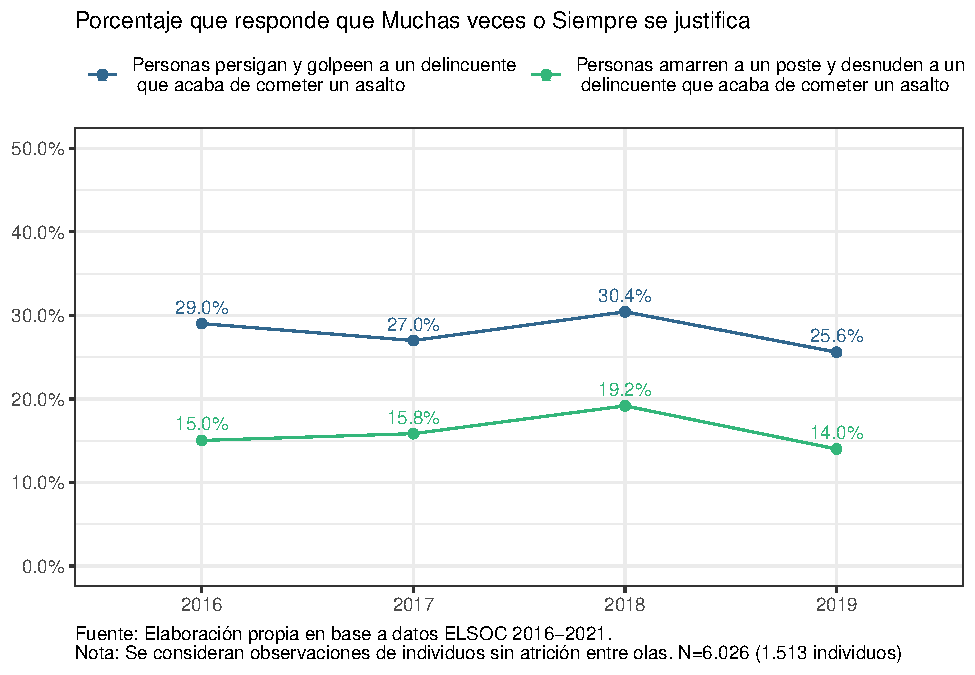
\includegraphics{reporte-elsoc_files/figure-latex/graf-justviolencia1-ola-1} 

}

\caption{Justificación de la violencia a manos de ciudadanos, según ola}\label{fig:graf-justviolencia1-ola}
\end{figure}

Tal como lo revela la Figura \ref{fig:graf-justviolencia2-ola}, por lo general, existe una baja justificación de la violencia policial en distintos contextos a lo largo del tiempo. Más concretamente, cuando se trata del uso de violencia para reprimir una marcha pacífica, durante el año de 2016, el 7\% de los encuestados reporta justificarse ``muchas veces o siempre'' el uso de la violencia. Esta justificación cae considerablemente el año 2019 (3.6\%) periodo en el cual ocurre el estallido social, sin embargo, registra una nueva alza llegando a un 6.1\% el año 2021.

Por otro lado, el uso de la violencia para desalojar a estudiantes de liceos en toma presenta un peak de justificación el año 2018 (17,9\%), reduciéndose de manera sustantiva el año 2019 llegando a sólo un 8.2\%, pero aumentando nuevamente a un 12.2\% el año 2021.

Al consultar sobre el uso de violencia policial cuando estudiantes tiran piedras a Carabineros en marchas por la educación, desde el año 2018 se registra un aumento constante de la justificación de este tipo de acción policial, pasando de 3.5\% justificable ``muchas veces o siempre'' ese año a 8.8\% el año 2021.

Resumidamente, en comparación con años anteriores, el año de 2019 existen menores niveles de justificación de la violencia policial en los tres contextos analizados, pero el año 2021, vuelve a aumentar el nivel de justificación de la violencia policial, un fenómeno que puede potencialmente atribuirse al contexto post estallido social y a una menor validación de la movilización social durante la pandemia.

\begin{figure}

{\centering 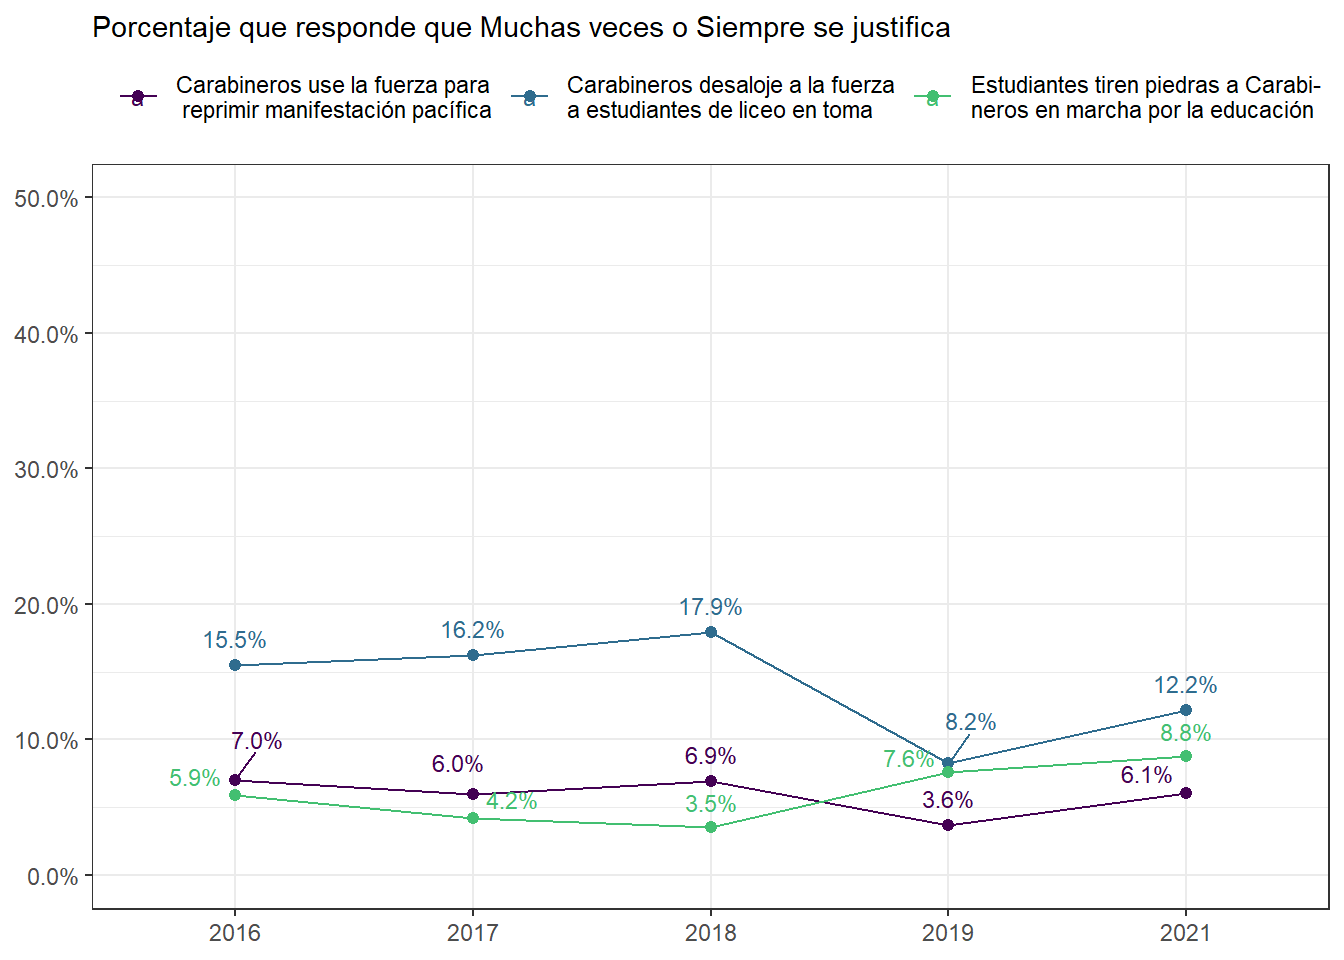
\includegraphics{reporte-elsoc_files/figure-latex/graf-justviolencia2-ola-1} 

}

\caption{Justificación de la violencia, según ola}\label{fig:graf-justviolencia2-ola}
\end{figure}

\hypertarget{confianza-interpersonal-y-en-instituciones}{%
\section{Confianza interpersonal y en instituciones}\label{confianza-interpersonal-y-en-instituciones}}

\hypertarget{confianza-interpersonal}{%
\subsection*{Confianza interpersonal}\label{confianza-interpersonal}}
\addcontentsline{toc}{subsection}{Confianza interpersonal}

Durante las últimas décadas, las ciencias sociales han acumulado mucha evidencia que muestra que la confianza social es un atributo social de mucha importancia y cin múltiples consecuencias. Entre otras cosas, se ha asociado con comportamientos prosociales y menor criminalidad (Uslaner, 2000), mayor crecimiento económico (Dincer \& Uslaner, 2010; Whiteley, 2000; Zak y Knack, 2001), mercados más eficientes (Fukuyama, 1996), democracias más robustas, y con mayor confianza en las instituciones (Newton \& Zmerli, 2011, Putnam et al., 1994). En este contexto, el registro longitudinal de ELSOC de la confianza social de la población adulta chilena resulta de mucha importancia.

El gráfico \ref{fig:graf-confianzainterpersonal-ola} muestra la evolución de dos indicadores comunes de confianza social durante cada ola de la encuesta. Se puede notar que en Chile el indicador que consulta acerca de cuán confiables son las personas desconocidas, el `otro' social imaginario, registra sistemáticamente niveles bajos que usualmente bordean el 12\%. Más preocupante aún, entre 2019 y 2021, la confianza social bajó del 11,4\% al 7,9\%, un nivel de decrecimiento que es observado por primera vez en ELSOC. Estas bajas podrían estar potencialmente asociadas a la creciente polazaciónpolarización que se observa en el país, así como a los efectos del distanciamiento social forzados por la pandemia del Coronavirus. La percepción de que las personas son justas presenta un registro más favorable con un nivel estable alrededor del 30\%.

\begin{figure}

{\centering 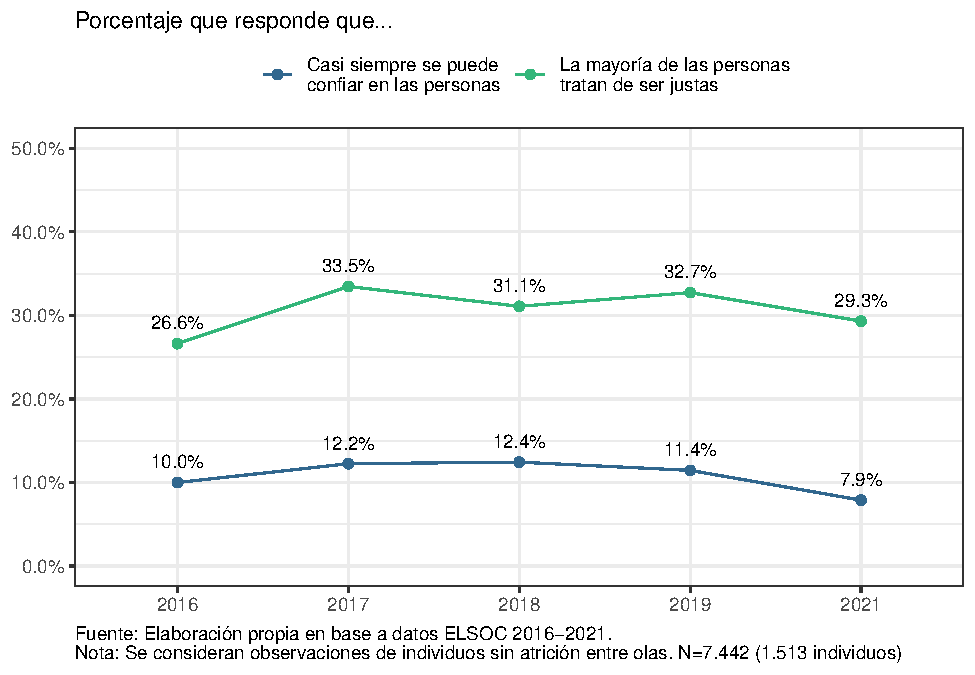
\includegraphics{reporte-elsoc_files/figure-latex/graf-confianzainterpersonal-ola-1} 

}

\caption{Confianza interpersonal, según ola}\label{fig:graf-confianzainterpersonal-ola}
\end{figure}

Detrás de la estabilidad temporal yace un gran nivel de diferenciación transversal en la confianza según distintos grupos socioeconómicos, particularmente educacionales. El gráfico \ref{fig:graf-confianzainterpersonal-educ} caracteriza la marcada desconfianza interpersonal en 2021, mostrando diferencias muy pronunciadas entre individuos con menor nivel educativo, que confían mucho menos y son más recelosos de cuán justos serán los demás,, e individuos con alto registro educacional registran mayor confianza en el otro y mayor percepción de comportamiento justo.

\begin{figure}

{\centering 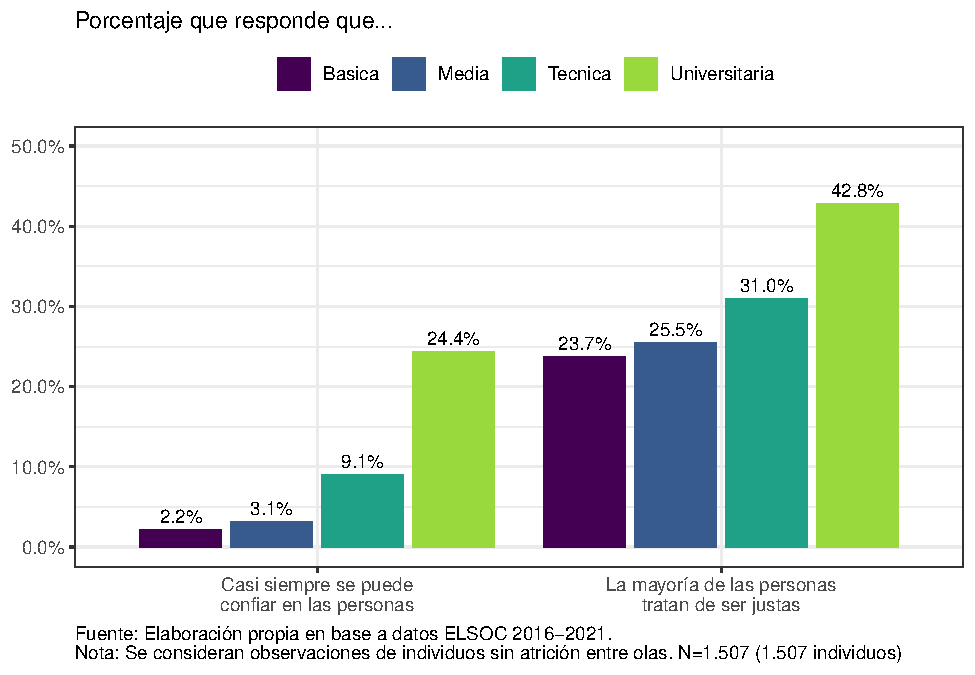
\includegraphics{reporte-elsoc_files/figure-latex/graf-confianzainterpersonal-educ-1} 

}

\caption{Confianza interpersonal (2021), según nivel educacional}\label{fig:graf-confianzainterpersonal-educ}
\end{figure}

\hypertarget{confianza-en-las-instituciones}{%
\subsection*{Confianza en las instituciones}\label{confianza-en-las-instituciones}}
\addcontentsline{toc}{subsection}{Confianza en las instituciones}

Las instituciones conforman los pilares organizacionales básicos de una sociedad, por lo que la estabilidad política está condicionada por la confianza que tienen los ciudadanos en las instituciones (Newton \& Norris, 1999). Por ello, parte de las explicaciones al estallido social de 2019 se fundan en la elevada desafección que existe con las instituciones políticas (Sehnbruch \& Donoso, 2020). Así, en el gráfico \ref{fig:graf-confinstituciones1-ola} y \ref{fig:graf-confinstituciones2-ola}, se observan dos patrones altamente relevantes. En primer lugar, el nivel de confianza en las instituciones, y las políticas en particular, son extremadamente bajas. Año tras año, el porcentaje de personas encuestadas que mencionan confiar `Mucho' o `Bastante' en el Congreso y Partidos Políticos no alcanza siquiera el 5\% de la población. Asimismo, el Poder Judicial y Presidente de la República registran durante sus mejores años niveles que apenas sobrepasan el 10\%. La única institución, que logra alcanzar niveles más elevados, sin desmedro de una pronunciada baja durante el periodo de observación, son Carabineros de Chile con un mínimo de confianza de 20,6\% en 2019 y 24,7\% en 2021.

Segundo, varias instituciones como el Congreso, Gobierno y Carabineros experimentan una pronunciada baja en la confianza el 2019. Las primeras dos instituciones incluso llegan a niveles ínfimos de un sólo dígito, presumiblemente asociado al Estallido Social, al tiempo que los niveles logran recuperarse levemente en 2021. No se observan vaivenes en los Partidos Políticos ya que los niveles de confianza ni siquiera alcanzan el 1\% en 2019 y 2020. Aunque las alzas constatadas durante la última ola son muy embrionarias, es posible que sean el resultado del proceso de cambio constitucional, que supone la elaboración de una nueva institución política -la Convención Constitucional- que involucró cambios relevantes en el sistema de representación, como la paridad de género, inclusión de escaños reservados a pueblos indígenas y la incorporación de listas completamente independientes de partidos políticos.

\begin{figure}

{\centering 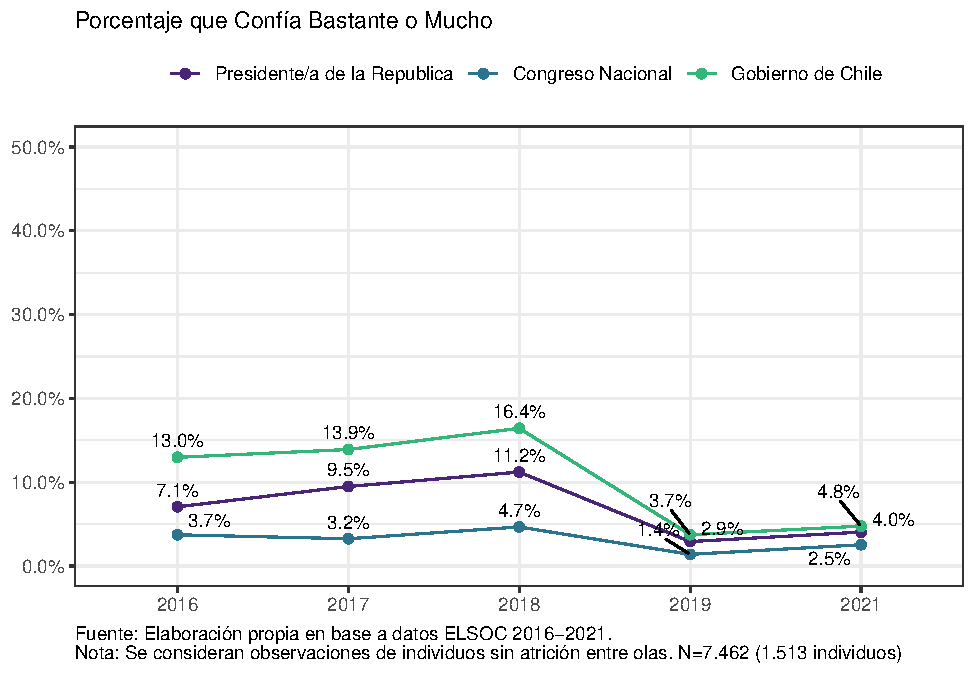
\includegraphics{reporte-elsoc_files/figure-latex/graf-confinstituciones1-ola-1} 

}

\caption{Grado de confianza en instituciones, según ola}\label{fig:graf-confinstituciones1-ola}
\end{figure}

\begin{figure}

{\centering 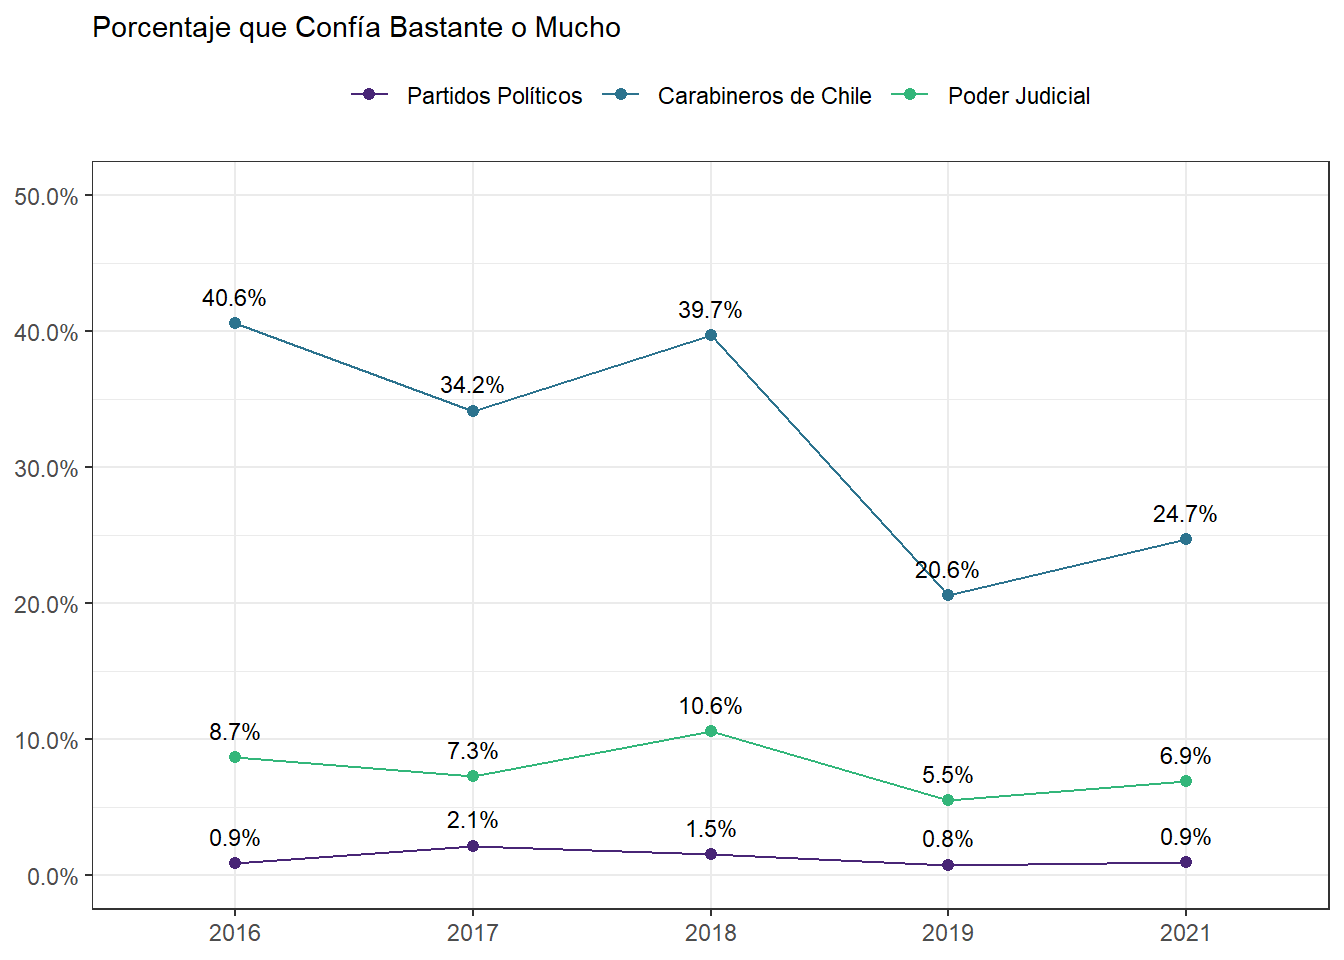
\includegraphics{reporte-elsoc_files/figure-latex/graf-confinstituciones2-ola-1} 

}

\caption{Grado de confianza en instituciones, según ola}\label{fig:graf-confinstituciones2-ola}
\end{figure}

\begin{figure}

{\centering 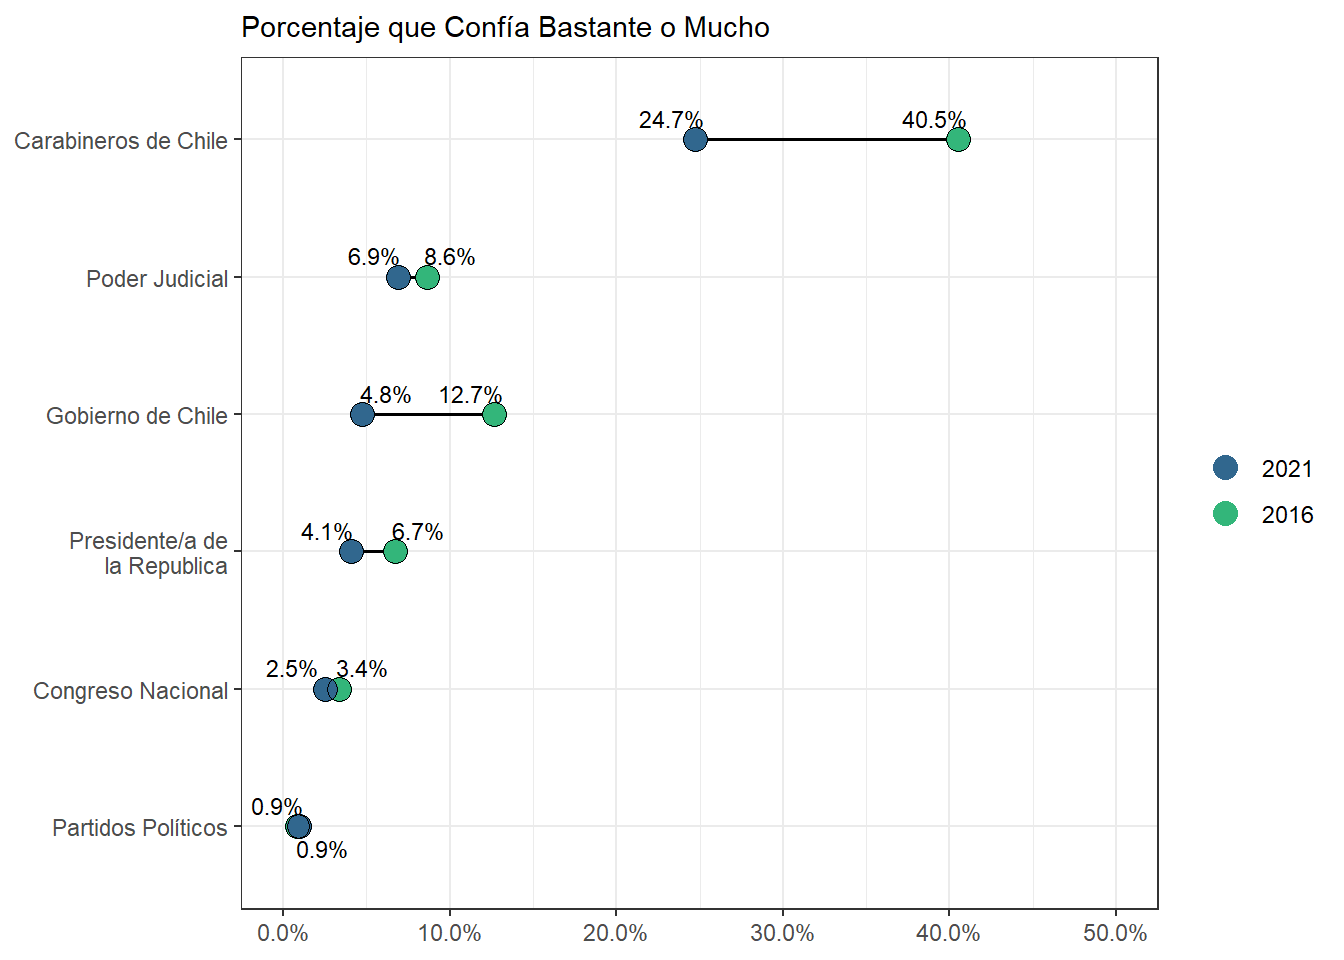
\includegraphics{reporte-elsoc_files/figure-latex/graf-cambio-confianzainstituciones-ola-1} 

}

\caption{Cambio en grado de confianza en instituciones (2016-2021)}\label{fig:graf-cambio-confianzainstituciones-ola}
\end{figure}

\hypertarget{actitudes-hacia-la-democracia}{%
\subsection{Actitudes hacia la democracia}\label{actitudes-hacia-la-democracia}}

La literatura ha distinguido entre el apoyo a los principios del régimen democrático y el respaldo a su desempeño (Easton, 1975; Norris, 1999). Así, el apoyo a la democracia como valor último se ha denominado legitimidad democrática, mientras que la evaluación del funcionamiento de la democracia constituye la satisfacción con la democracia. El gráfico \ref{fig:graf-preferenciademocracia-ola} muestra que en Chile se consolida el fenómeno global del ciudadano crítico (Norris, 1999), que refiere a individuos altamente comprometidos con la democracia como regimen político, superando niveles del 50\%, aunque también altamente insatisfechos con su funcionamiento, pues desde 2019 la satisfacción con la democracia no supera el 6\%.

\begin{figure}

{\centering 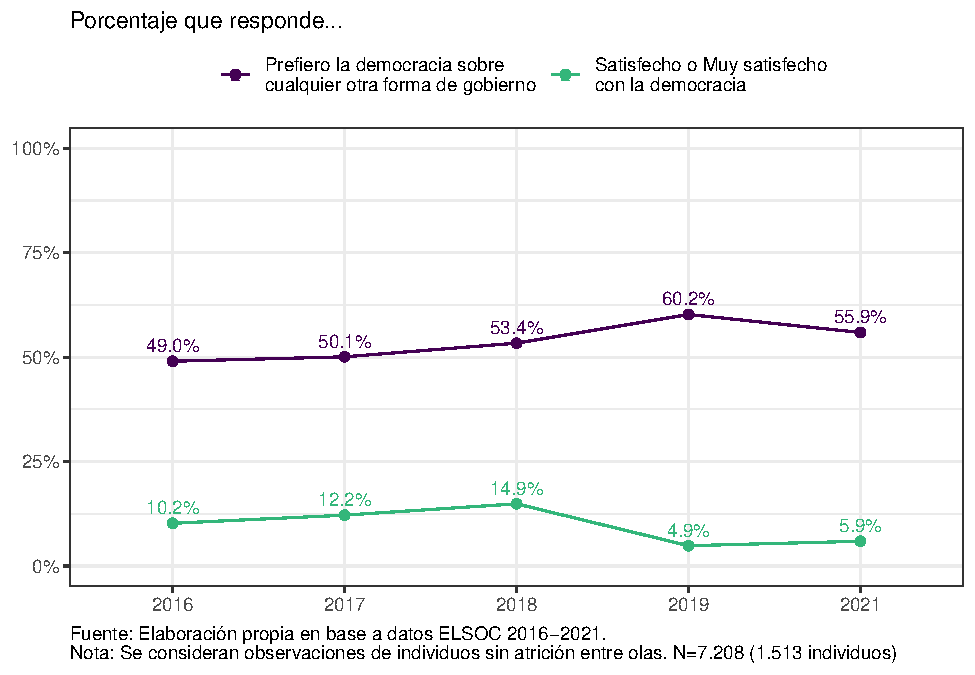
\includegraphics{reporte-elsoc_files/figure-latex/graf-preferenciademocracia-ola-1} 

}

\caption{Preferencia por y satisfacción con la democracia, según ola}\label{fig:graf-preferenciademocracia-ola}
\end{figure}

El gráfico \ref{fig:graf-preferenciademocracia-idpolitica} y \ref{fig:graf-preferenciademocracia2-idpolitica} indican que el fenómeno del ciudadano crítico es transversal a la identificación en el espectro izquierda-derecha, aunque se presenta más marcadamente en sujetos identificados con la izquierda que legitiman en un 74,8\% la democracia y solo un 4,1\% está satisfecho o muy satisfecho con su funcionamiento. En contraste, los individuos de derecha tienen una menor legitimidad democrática, del 38,7\%, al tiempo que un 8,9\% está satisfecho o muy satisfecho con su funcionamiento.

\begin{figure}

{\centering 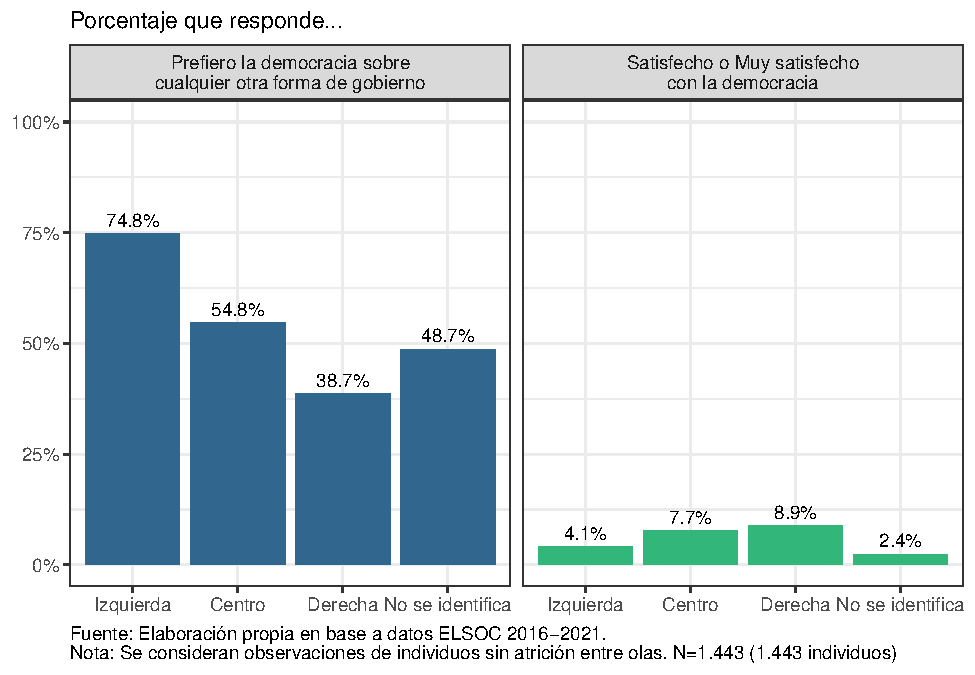
\includegraphics{reporte-elsoc_files/figure-latex/graf-preferenciademocracia-idpolitica-1} 

}

\caption{Preferencia por y satisfacción con la democracia (2021), según posición ideológica}\label{fig:graf-preferenciademocracia-idpolitica}
\end{figure}

\begin{figure}

{\centering 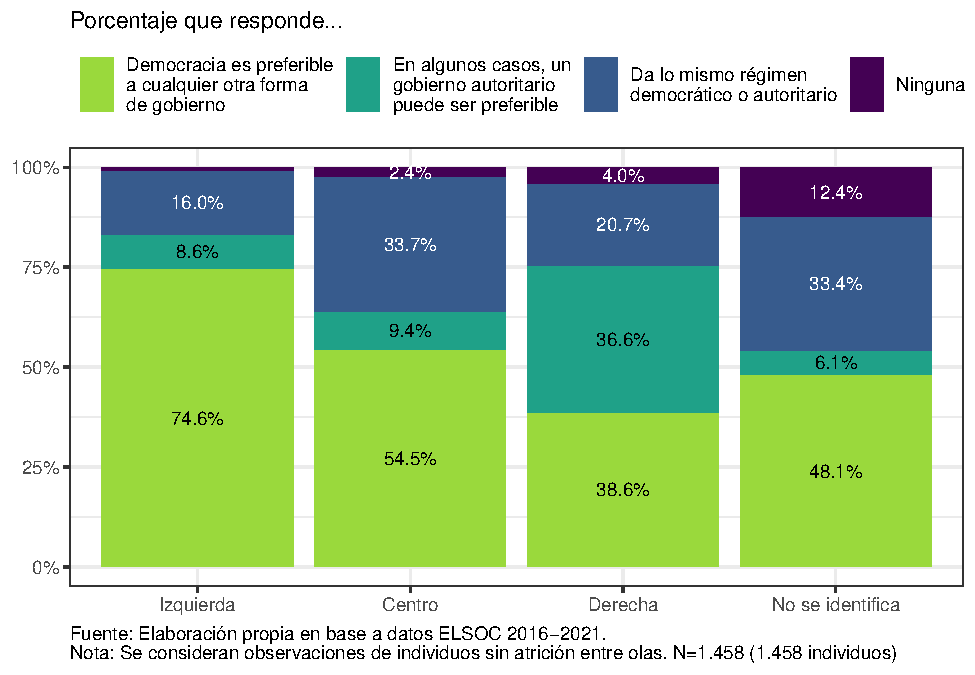
\includegraphics{reporte-elsoc_files/figure-latex/graf-preferenciademocracia2-idpolitica-1} 

}

\caption{Preferencia por la democracia (2021), según posición ideológica}\label{fig:graf-preferenciademocracia2-idpolitica}
\end{figure}

\hypertarget{participaciuxf3n-electoral}{%
\section{Participación electoral}\label{participaciuxf3n-electoral}}

Con el inicio del proceso constituyente, durante 2020 y 2021 se realizaron procesos electorales novedosos en el país, los que combinados con los efectos de la pandemia, pudieron haber alterado el comportamiento electoral de los ciudadanos. El gráfico \ref{fig:graf-participelect-ola} muestra que existe un sobre-reporte de haber participado en elecciones, cuestión que coincide con la literatura de encuestas (Silver et al., 1986). Mientras que en el plebiscito participó un 50,9\% del padrón electoral, ELSOC reporta un 68,6\%, sobrerrepresentación que parece mantenerse estable elección a elección. No obstante, el gráfico \ref{fig:graf-servel-apruebo} muestra que ELSOC se acerca bastante a la realidad al medir la intención de voto retrospectiva, con una diferencia de sólo 5\% al predecir el apruebo respecto a los datos del SERVEL.

\begin{figure}

{\centering 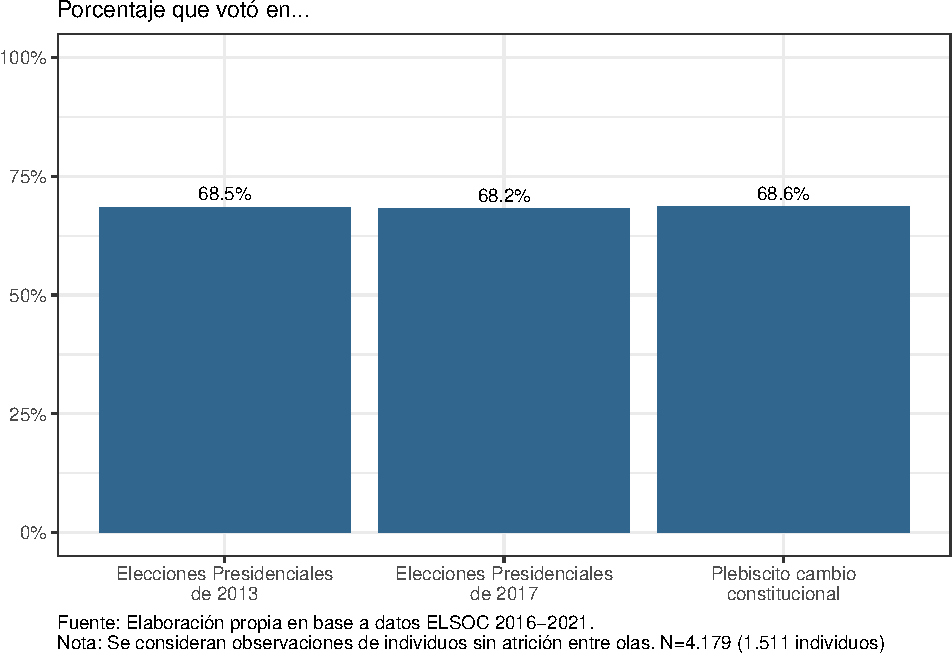
\includegraphics{reporte-elsoc_files/figure-latex/graf-participelect-ola-1} 

}

\caption{Participación electoral, según elección}\label{fig:graf-participelect-ola}
\end{figure}

\begin{figure}

{\centering 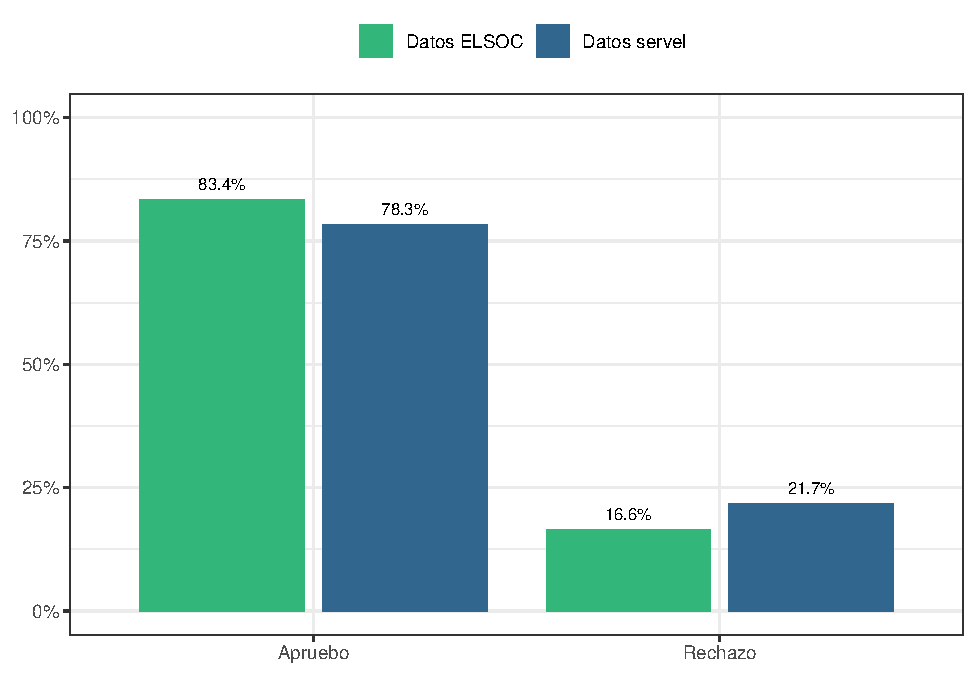
\includegraphics{reporte-elsoc_files/figure-latex/graf-servel-apruebo-1} 

}

\caption{Voto retrospectivo Plebiscito Nueva Constitucion}\label{fig:graf-servel-apruebo}
\end{figure}

El gráfico \ref{fig:graf-participelect-olas-edad} muestra que los patrones de participación electoral se vieron fuertemente alterados con el advenimiento de la pandemia y el proceso constituyente. La participación entre los adultos y adultos mayores se redujo considerablemente, mientras que aumentó la participación de personas menores de 49 años. Mientras que el 91\% de los mayores de 65 años mencionaron haber votado en la elección del 2013, esta cifra se reduce a un 67\% en el Plebiscito de 2020. En cambio los jóvenes de 18 a 29 años ascienden su participación desde un 53\% en 2013 hasta un 75\% en 2020. Esto constituye un severo cambio en la composición del electorado, pero cuya continuidad en el tiempo es aún desconocida.

\begin{figure}

{\centering 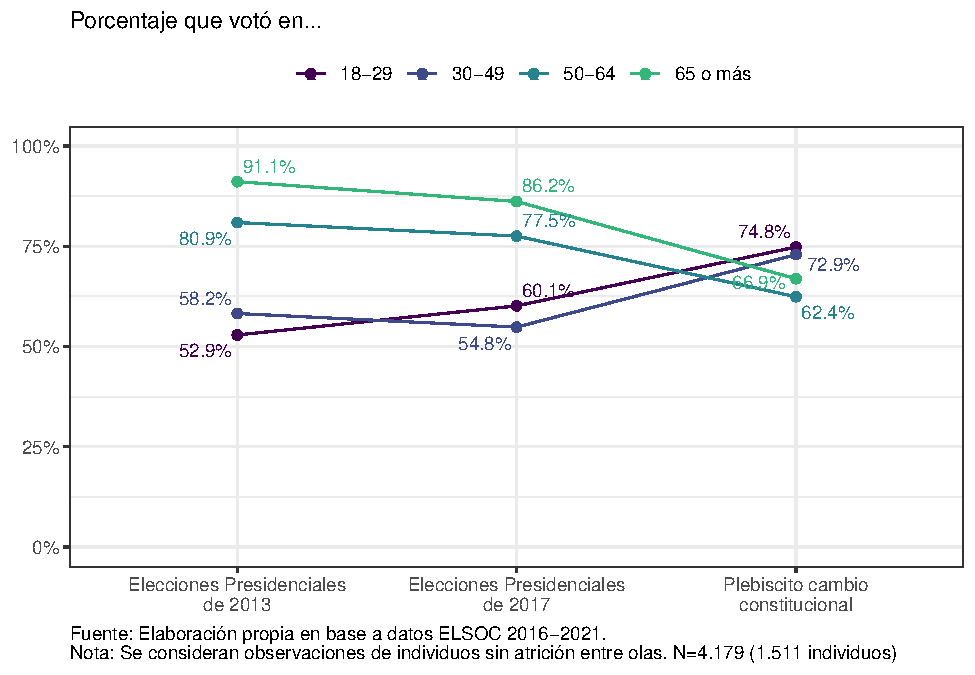
\includegraphics{reporte-elsoc_files/figure-latex/graf-participelect-olas-edad-1} 

}

\caption{Participación electoral, según tramo de edad}\label{fig:graf-participelect-olas-edad}
\end{figure}

En términos de preferencias ideológicas, el gráfico \ref{fig:graf-votoplebiscito-idpolitica} muestra que la opción por el apruebo fue más votada entre los sujetos identificados con la izquierda, con un 80,2\% comparado con un 46,7\% entre quienes se identifican con la derecha. También se producen diferencias importantes en los niveles de abstención entre grupos ideológicos, donde un 18\% de las personas que se identifican con la izquierda no votaron, cifra que asciende a un 36\% y 32\% entre las personas de centro y derecha, respectivamente. Esto es consistente con la idea de que la promesa de una transformación institucional se convirtió en fuerte motivante de participación. Los niveles de apoyo a la opción del Apruebo según tendencia ideológica se reiteran en el gráfico \ref{fig:graf-voto-votoprevio} que muestra que quienes votaron por candidatos de izquierda en elecciones pasadas también tendieron a votar de sobremanera por el apruebo. Por otro lado, el gráfico \ref{fig:graf-voto-votopresi} robustece la idea del voto como hábito, pues quienes votaron en elecciones anteriores participaron del plebiscito en mayor proporción.

\begin{figure}

{\centering 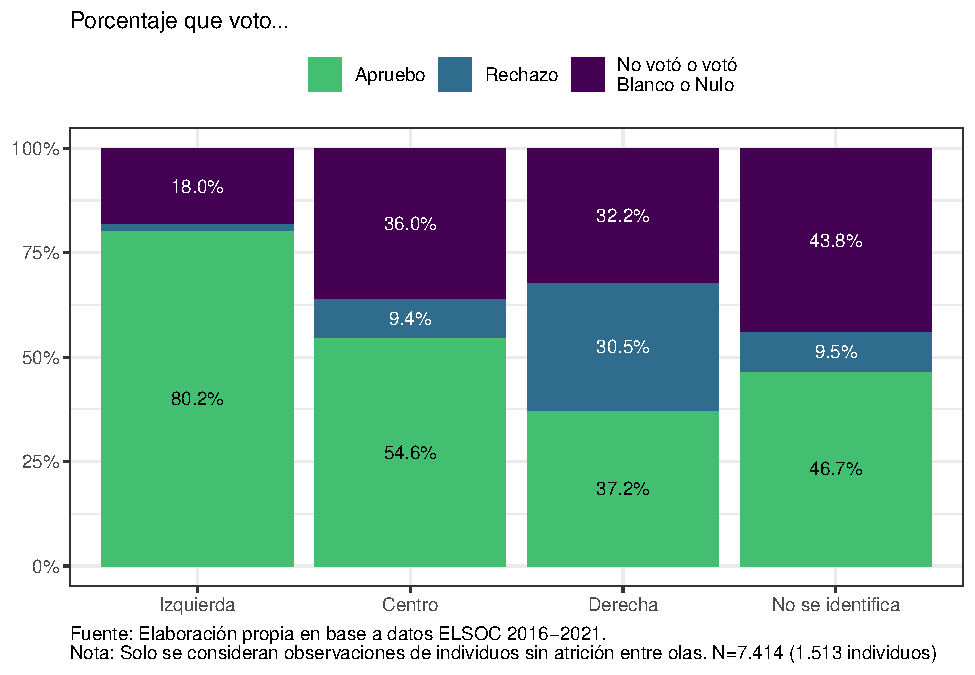
\includegraphics{reporte-elsoc_files/figure-latex/graf-votoplebiscito-idpolitica-1} 

}

\caption{Voto en plebiscito de 2020, según identificación política}\label{fig:graf-votoplebiscito-idpolitica}
\end{figure}

\begin{figure}

{\centering 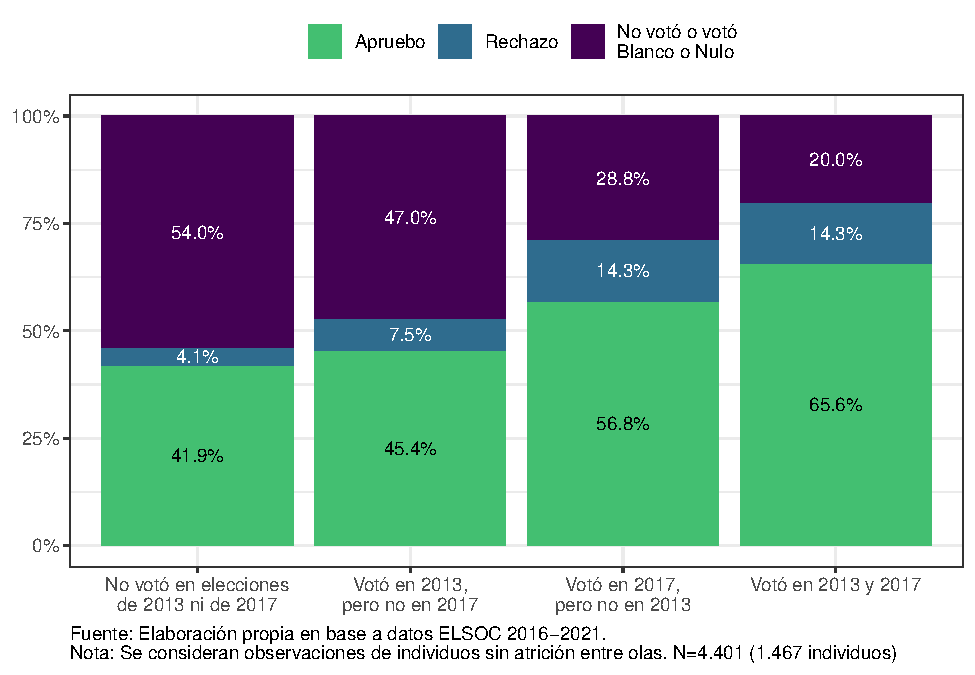
\includegraphics{reporte-elsoc_files/figure-latex/graf-voto-votoprevio-1} 

}

\caption{Voto en plebiscito de 2020, según voto en elecciones previas}\label{fig:graf-voto-votoprevio}
\end{figure}

\begin{figure}

{\centering 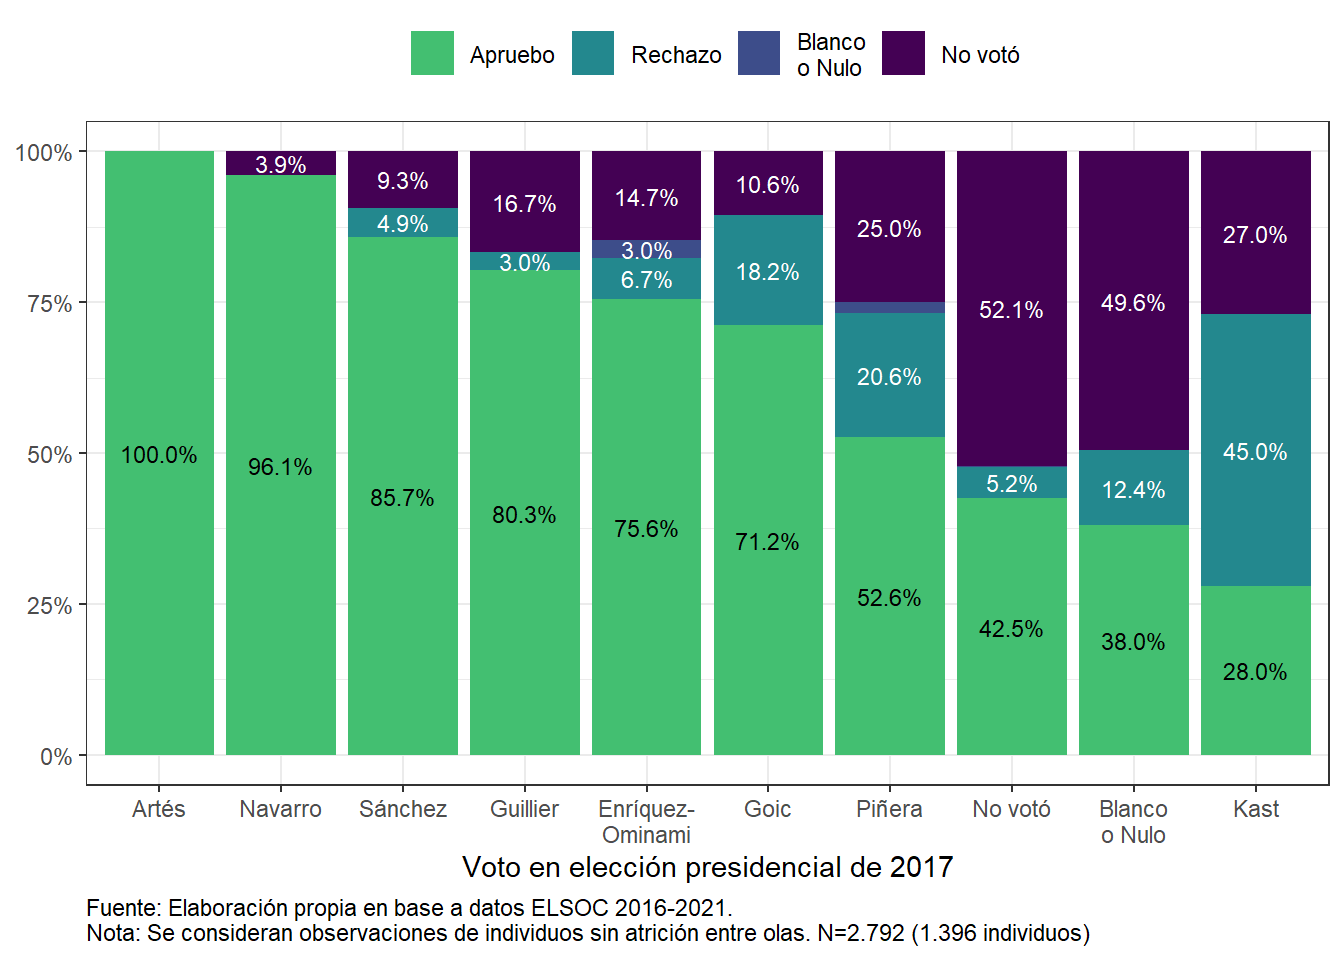
\includegraphics{reporte-elsoc_files/figure-latex/graf-voto-votopresi-1} 

}

\caption{Voto en plebiscito de 2020, según voto en elección presidencial de 2017}\label{fig:graf-voto-votopresi}
\end{figure}

\hypertarget{proceso-constituyente}{%
\section{Proceso Constituyente}\label{proceso-constituyente}}

El plebiscito de 2020 dió inicio al proceso constituyente con un resultado del 78,31\% por el apruebo y 79,18\% por la opción de una Convención Constitucional. Pese a la magnitud del triunfo, la mediatización del cambio constitucional ha generado diversas posturas sobre el proceso en la opinión pública. El gráfico \ref{fig:graf-optimismoconstitucional} muestra que existen altos niveles de optimismo respecto a los efectos que tendrá el proceso constitucional sobre la sociedad chilena. Un 62\% de las personas encuestadas está de acuerdo o muy de acuerdo con que el proceso constituyente reducirá la desigualdad y un 50,2\% con que disminuirá la corrupción. En contraste, los ítem que reflejan un prospecto desfavorable encuentran menor apoyo; un 33\% de personas que están de acuerdo o muy de acuerdo con que impactará poco en la calidad de vida y un 22,9\% considera que empeorará las condiciones económicas. Como es de esperar, los gráficos \ref{fig:graf-optimismoconstitucional-votoplebiscito} y \ref{fig:graf-optimismoconstitucional-educ} muestran que existe un mayor nivel de optimismo entre quienes votaron apruebo (72,7\%), al tiempo que el optimismo es similar entre grupos educativos. En el gráfico \ref{fig:graf-optimismoconstitucional-idpolitica} se observa que la izquierda y las personas sin identificación política tienen los mayores niveles de optimismo, 72,7\% y 66,9\% respectivamente, en contraste al 61,4\% del centro y el 44,8\% de la derecha.

\begin{figure}

{\centering 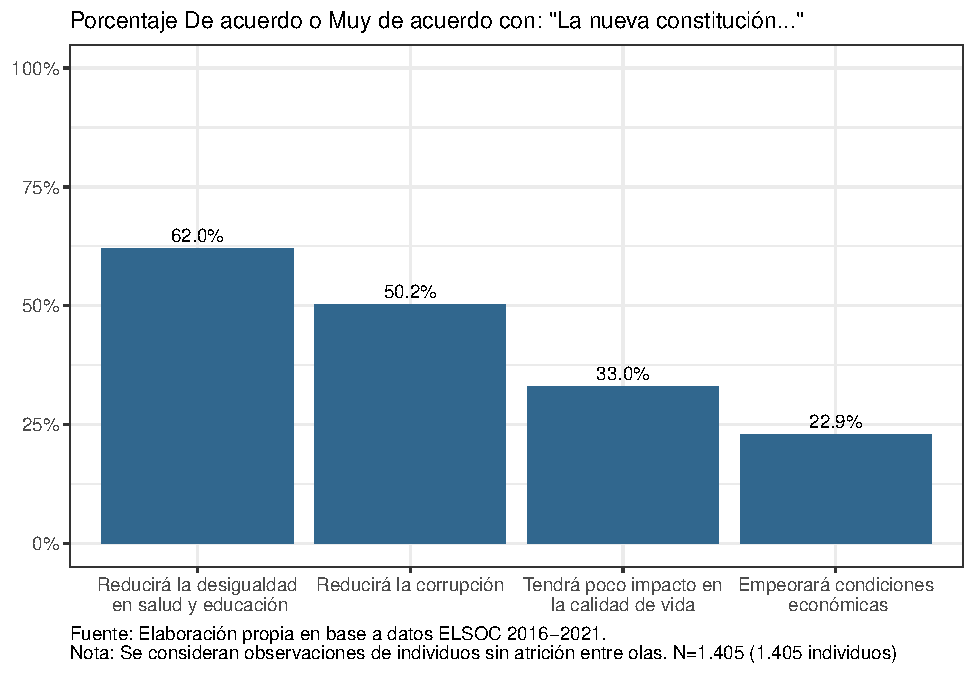
\includegraphics{reporte-elsoc_files/figure-latex/graf-optimismoconstitucional-1} 

}

\caption{Optimismo constitucional}\label{fig:graf-optimismoconstitucional}
\end{figure}

\begin{figure}

{\centering 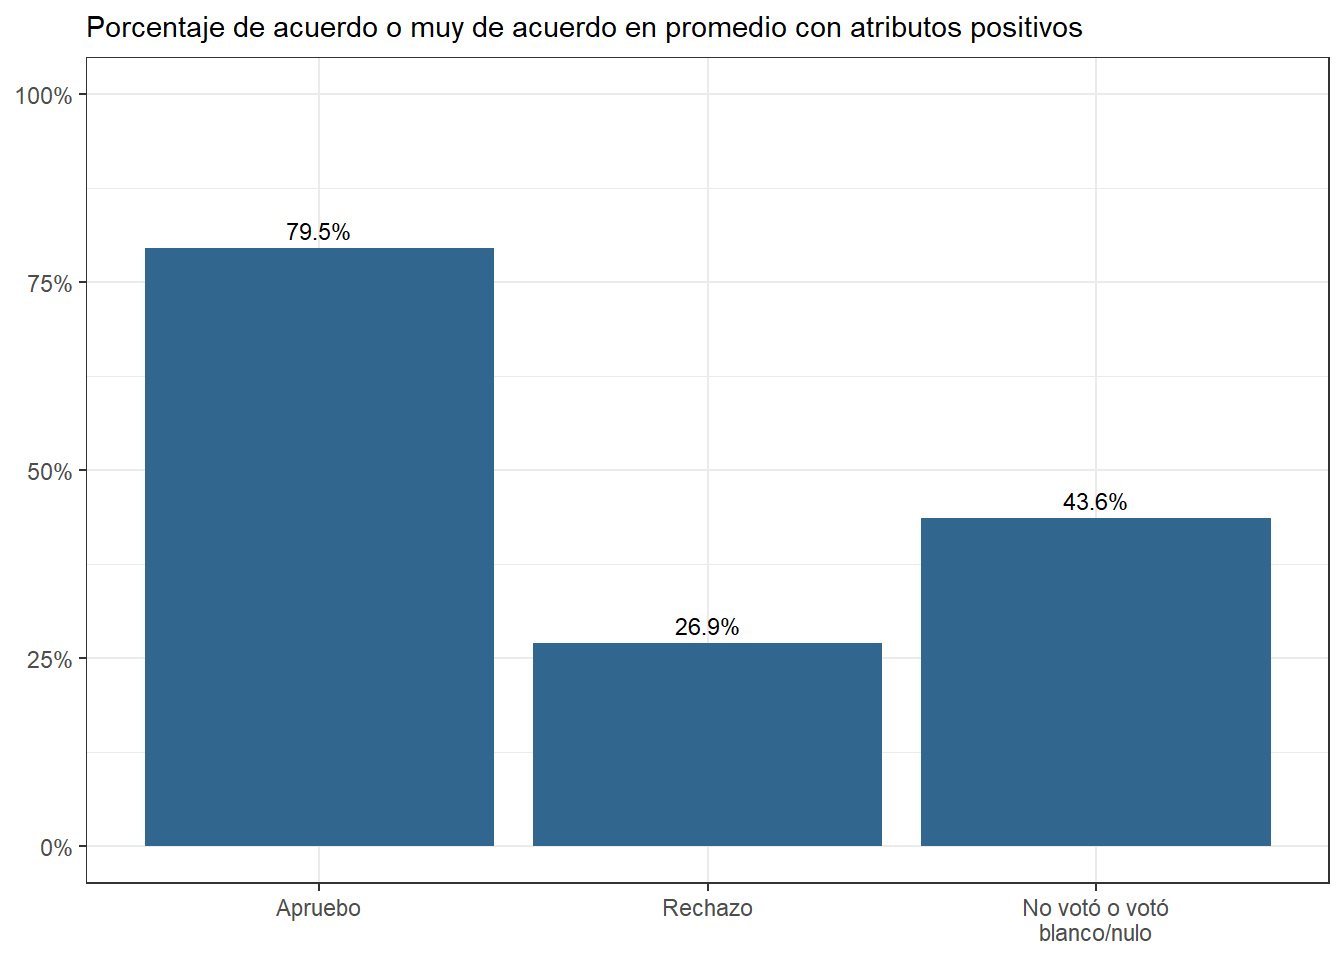
\includegraphics{reporte-elsoc_files/figure-latex/graf-optimismoconstitucional-votoplebiscito-1} 

}

\caption{Optimismo constitucional, según voto en plebiscito de 2020}\label{fig:graf-optimismoconstitucional-votoplebiscito}
\end{figure}

\begin{figure}

{\centering 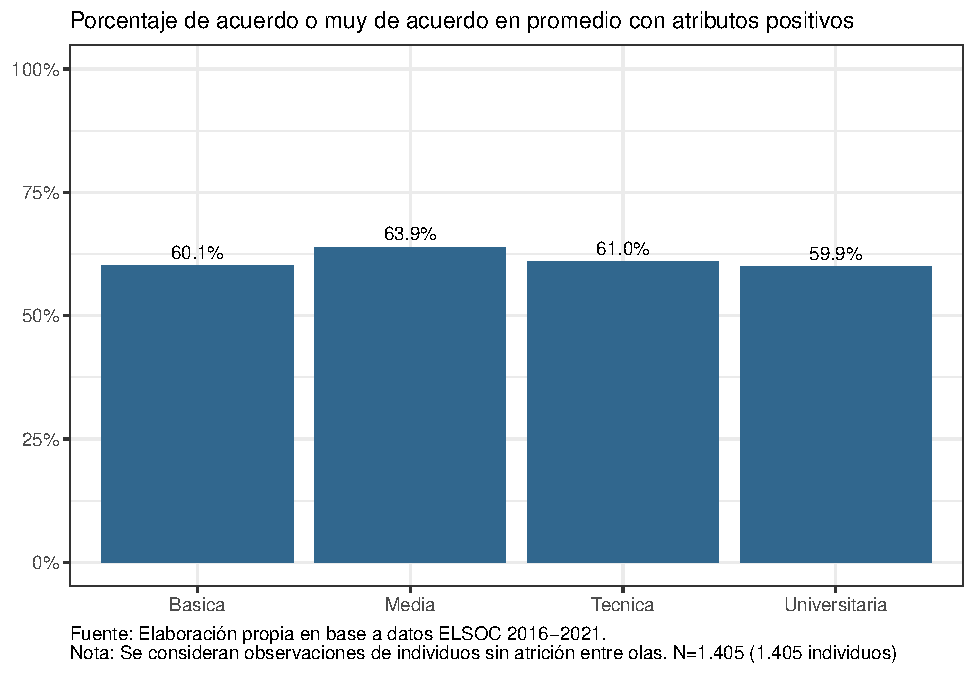
\includegraphics{reporte-elsoc_files/figure-latex/graf-optimismoconstitucional-educ-1} 

}

\caption{Optimismo constitucional, según nivel educacional}\label{fig:graf-optimismoconstitucional-educ}
\end{figure}

\begin{figure}

{\centering 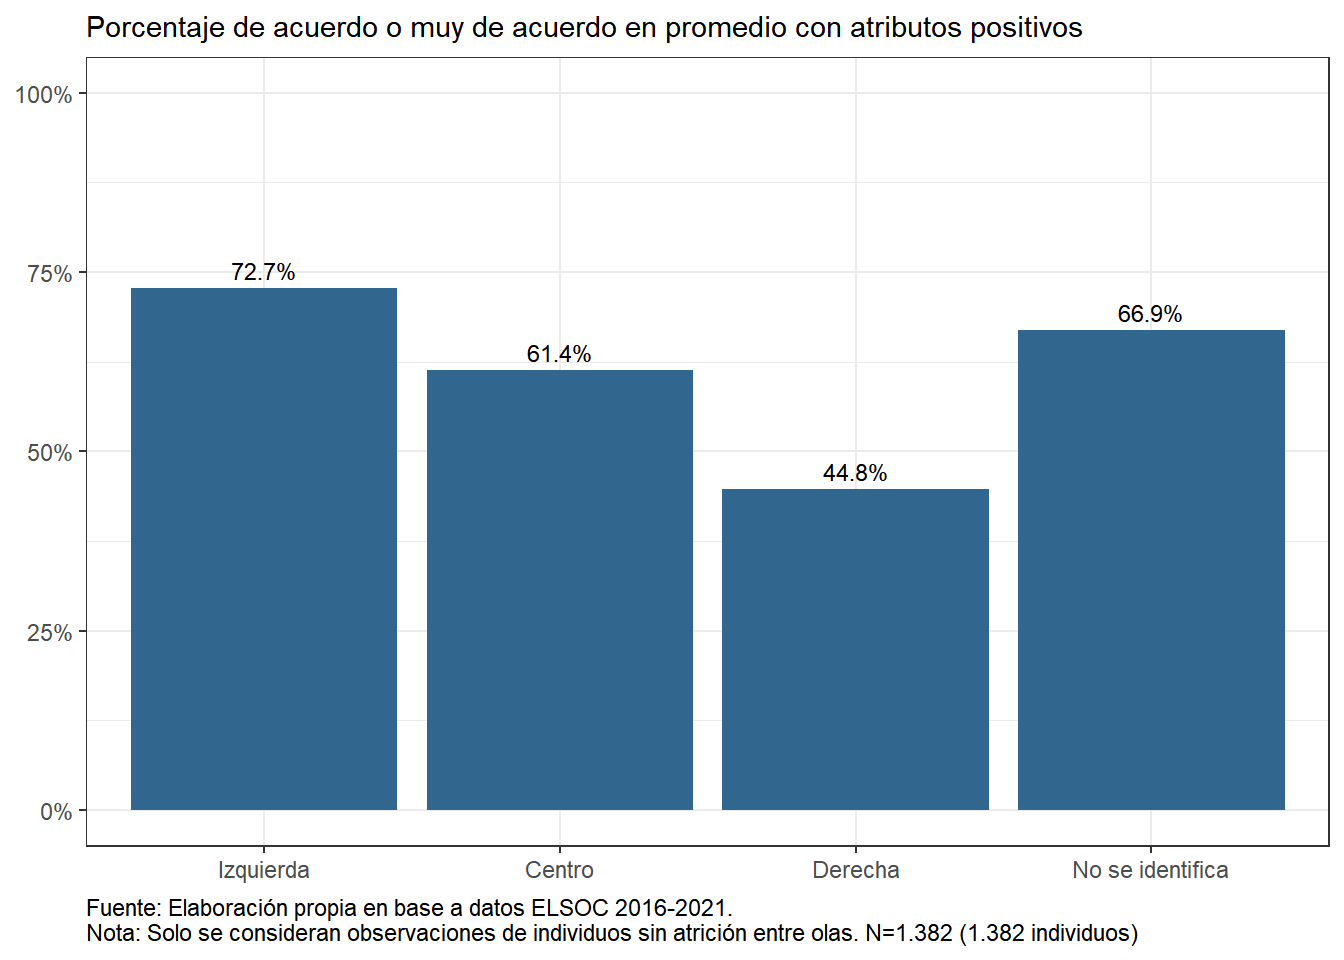
\includegraphics{reporte-elsoc_files/figure-latex/graf-optimismoconstitucional-idpolitica-1} 

}

\caption{Optimismo constitucional, según identificación política}\label{fig:graf-optimismoconstitucional-idpolitica}
\end{figure}

\hypertarget{salud-mental-y-bienestar}{%
\chapter{Salud mental y bienestar}\label{salud-mental-y-bienestar}}

\hypertarget{salud-mental-y-bienestar-1}{%
\section{Salud mental y bienestar}\label{salud-mental-y-bienestar-1}}

Chile es un país que se caracteriza por una carga de trastornos mentales relativamente alta con escaso acceso a servicios de salud mental (Vicente et al, 2016). La irrupción de significativos fenómenos locales y globales, como el Estallido Social ocurrido a partir de octubre de 2019 y sus repercusiones políticas e institucionales, así como la pandemia por COVID-19 y las medidas para contenerla, con sus impactos en la salud, condiciones económicas y de sociabilidad de la población; han tenido un marcado efecto sobre la salud mental y el nivel de bienestar de la población (Wu et al, 2021; Duarte \& Jiménez, 2021).

A pesar de las difíciles condiciones sanitarias y económicas, los datos ELSOC nos permiten señalar que la población chilena presenta aún un alto porcentaje de satisfacción con la vida: 83,7\% responde estar satisfecho o muy satisfecho con su vida (Figura \ref{fig:salud-bienestar-2021}), y 63,5\% responde que su vida se acerca o se acerca completamente a su ideal.

Esto es consistente con los datos de otras encuestas realizadas en contexto pre-pandémico o pandémico. Lo que muestran encuestas previas, como la Encuesta de Desarrollo Humano del 2011 (PNUD, 2012) o la encuesta Termómetro Social de octubre 2020 (DESOC-COES, 2020) es que, en general, los chilenos están satisfechos con sus vidas.

Por otra parte, y en contraste, solo un 15,8\% indicó en 2021 que su salud es muy buena o excelente.

\begin{figure}

{\centering 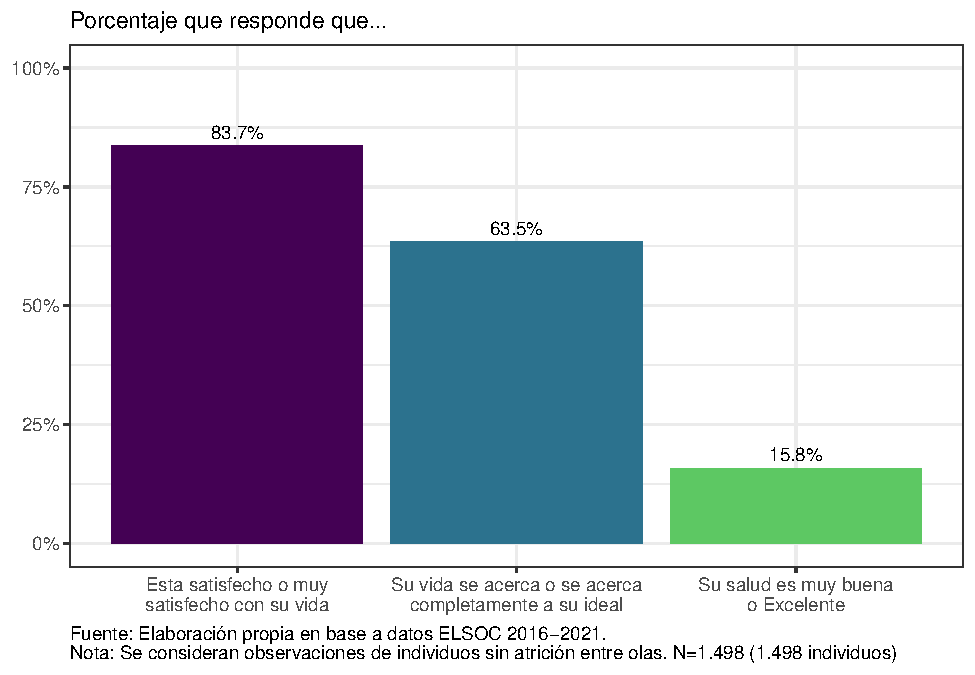
\includegraphics{reporte-elsoc_files/figure-latex/salud-bienestar-2021-1} 

}

\caption{Satisfacción con la vida, ideal de vida y salud subjetiva (ola 2021)}\label{fig:salud-bienestar-2021}
\end{figure}

Al analizar la evolución de estos indicadores, encontramos dos fenómenos que destacan: una fuerte caída en términos de salud subjetiva y satisfacción con la vida durante 2019; y una más fuerte y, quizás contraintuitiva, recuperación a partir de 2021.

El 2019 el porcentaje que reporta estar satisfecho o muy satisfecho con su vida cae a 70,4\% (desde 79,4\% el 2018), y a 55,0\% entre quienes indican que su vida se acerca o se acerca completamente a su ideal (desde 62,7\%). Estos fenómenos se encuentran probablemente asociados al contexto estallido social ocurrido a partir de octubre de 2019 (encuesta fue realizada a partir de noviembre de 2019).

Por otra parte, el 2021 se aprecia un marcado aumento en la satisfacción y acercamiento al ideal de vida, llegando a porcentajes superiores a niveles previos a 2019: 83,7\% y 63,5\%, respectivamente. Estos resultados resultan particularmente contraintuitivos, ya que existe evidencia que muestra un deterioro en la calidad de vida de la población y una percepción de mayor vulnerabilidad durante la pandemia (DESOC-COES, 2020). Sin embargo, es posible que este resultado se encuentre asociado a la mejoría en la situación sanitaria del país al momento en que fue realizada la encuesta (a partir de febrero de 2021), pero también a fenómenos de resiliencia o aumento de la solidaridad social ante situaciones adversas, como ha reportado literatura internacional durante la pandemia (Bavel et al, 2020).

\begin{figure}

{\centering 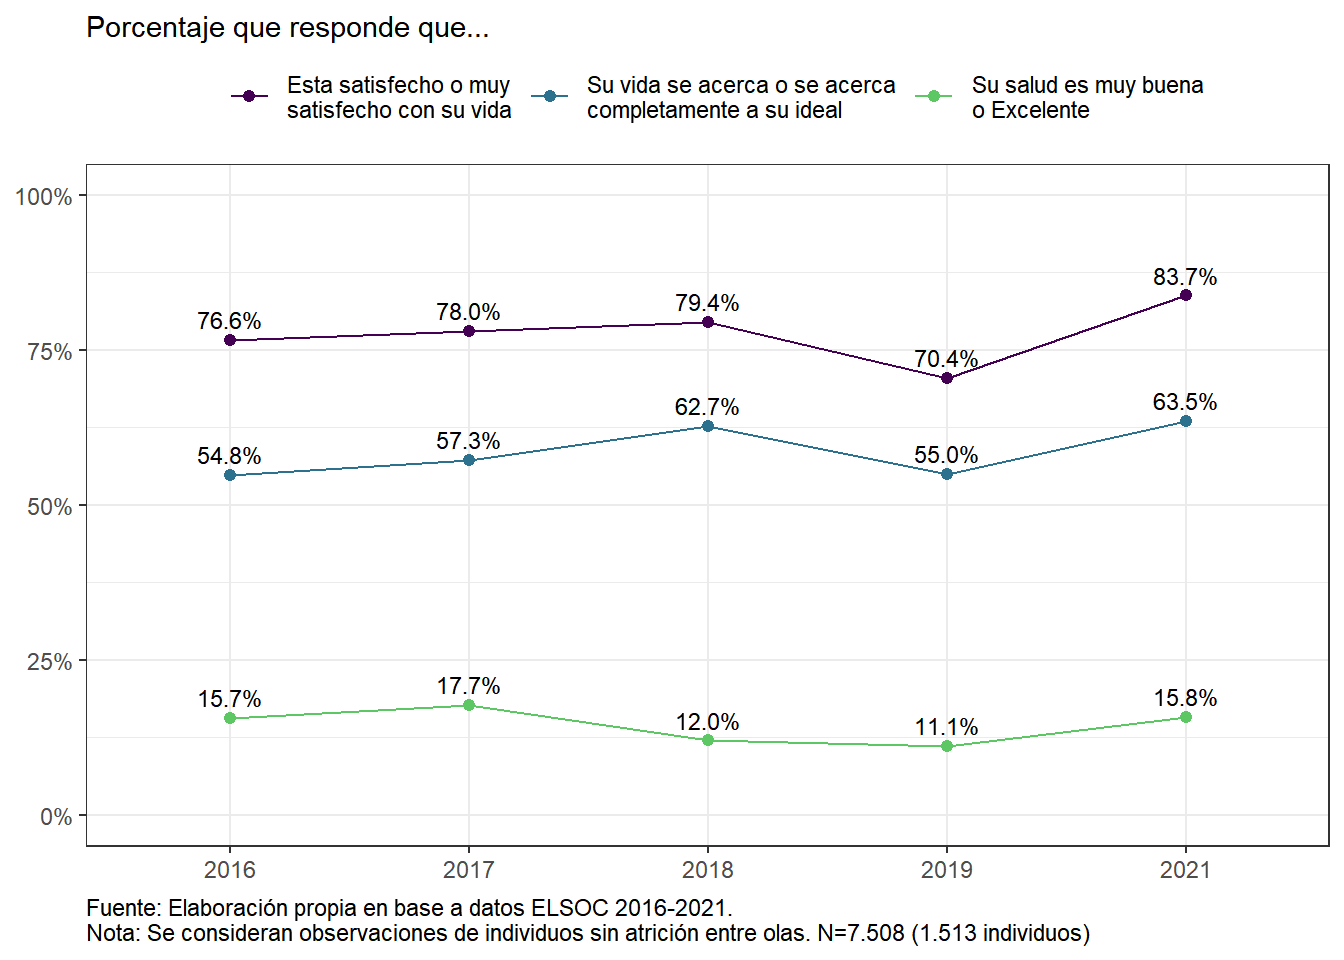
\includegraphics{reporte-elsoc_files/figure-latex/salud-bienestar-olas-1} 

}

\caption{Satisfacción con la vida, ideal de vida y salud subjetiva, según ola}\label{fig:salud-bienestar-olas}
\end{figure}

\hypertarget{sintomatologuxeda-depresiva}{%
\subsection*{Sintomatología depresiva}\label{sintomatologuxeda-depresiva}}
\addcontentsline{toc}{subsection}{Sintomatología depresiva}

En cuanto a sintomatología depresiva, ELSOC utiliza la escala PHQ-9 (Patient Health Questionnaire), un cuestionario de autorreporte que permite establecer la presencia y severidad de los síntomas\footnote{Debido al contexto de pandemia, en 2021 la escala PHQ-9 no fue aplicada como un cuestionario de auto reporte}. Si bien no es un instrumento de diagnóstico, ha demostrado una buena precisión diagnóstica (Kroenke et al, 2001; Levis et al, 2019) y ha sido validado para la población chilena (Baader et al, 2012).

Los resultados de la escala PHQ-9 son clasificados en 4 categorías, según la presencia y habitualidad de síntomas depresivos: de 0-9 se considera ``Sin síntomas o con síntomas depresivos mínimos,'' de 10-14 ``Sintomatología depresiva media''; de 15-19 ``Sintomatología depresiva moderada'' y de 20-27 ``Sintomatología depresiva moderada-severa o severa.''

Los resultados de 2021 muestran que, si bien un 48,6\% de la población no presenta o presenta síntomas mínimos de depresión (Figura \ref{fig:depre-2021}), un alto porcentaje presenta síntomas depresivos, en distintos niveles de severidad. Un 32,6\% de la población presenta sintomatología depresiva media, 11,2\% síntomas depresivos moderados, y 7,7\% de depresión moderada-severa a severa (Figura \ref{fig:depre-2021}), lo que revela una alta prevalencia de este tipo de síntomas en la población general y confirma una deteriorada situación de la salud mental en Chile.

\begin{figure}

{\centering 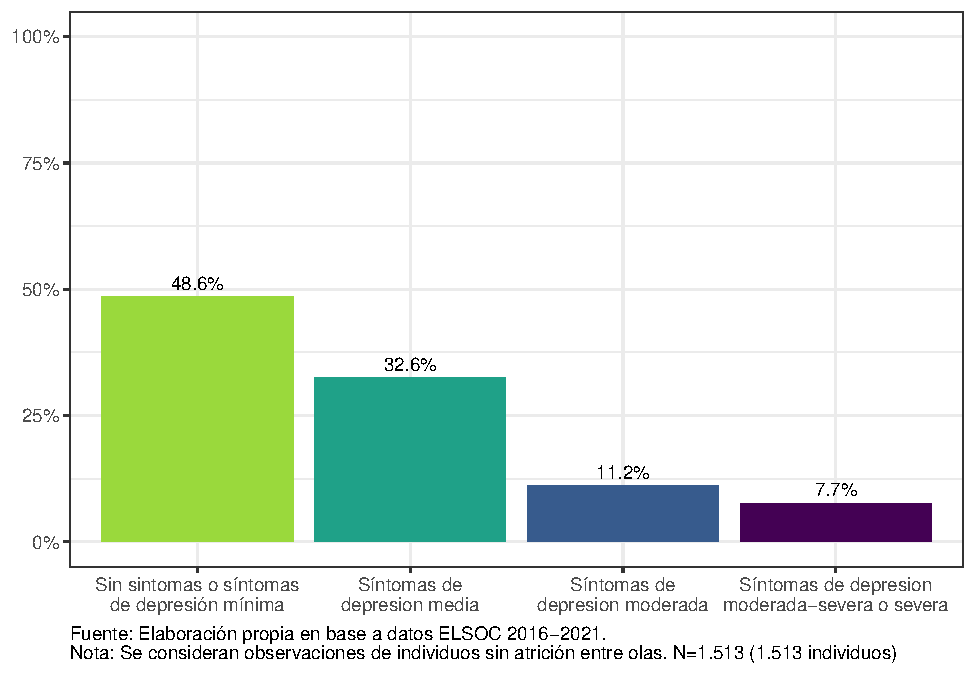
\includegraphics{reporte-elsoc_files/figure-latex/depre-2021-1} 

}

\caption{Porcentaje que presenta síntomas de depresión (2021)}\label{fig:depre-2021}
\end{figure}

Como es de esperar, la existencia de síntomas depresivos se encuentra altamente correlacionada con la satisfacción con la vida y con el porcentaje que considera que su vida se acerca a su ideal: un 93,2\% de aquellos y aquellas que no presentan síntomas depresivos se encuentran satisfechos o muy satisfechos con su vida, mientras que este porcentaje se reduce a 53,8\% entre aquellos que presentan sintomatología depresiva moderada-severa a severa. Ahora bien, este último resultado podría parecer paradojal, puesto que se trata de un grupo de personas que se encuentran satisfechas con sus vidas pero al mismo tiempo sufren un estado depresivo, caracterizado por intensa tristeza. Esta aparente paradoja podría explicarse a partir del modelo de ``dos continuos'' (Westerhof \& Keyes, 2010; Kinderman et al, 2015), en el cual los trastornos mentales (como la depresión) y la salud mental y bienestar están relacionados, pero son dimensiones diferentes (un continuo indica la presencia o ausencia de salud mental y bienestar subjetivo, mientras que el otro indica la presencia o ausencia de psicopatología). Esto permite entender que personas con un mismo nivel de severidad de síntomas puedan tener diferentes niveles de adaptación psicosocial, y un impacto diferente en la calidad de vida y satisfacción con la misma.

\begin{figure}

{\centering \includegraphics{reporte-elsoc_files/figure-latex/depre-bienestar-1} 

}

\caption{Satisfacción con la vida, ideal de vida y salud subjetiva (ola 2021), según Sintomas de depresión}\label{fig:depre-bienestar}
\end{figure}

Al igual que en términos de satisfacción con la vida, la prevalencia de síntomas depresivos aumentó el año 2019, en particular la prevalencia de sintomatología depresiva media, al pasar de 33,0\% a 40,9\% entre 2018 y 2019. Asimismo, la relativamente alta prevalencia de síntomas depresivos moderados a severos en 2019 (25,1\%) parece mostrar un efecto importante y negativo del contexto de estallido social sobre la salud mental de la población. Este resultado se encuentra en sintonía con la literatura internacional. De hecho, se estima que después de grandes protestas sociales la prevalencia de depresión aumenta en torno a 7\% (Ni et al, 2020), lo cual refleja un impacto comparable a los de los desastres naturales o conflictos armados. Un estudio longitudinal realizado en Hong Kong mostró que la depresión y los síntomas de estrés postraumático aumentaron significativamente luego del estallido social ocurrido a principios de 2019 en dicho país (Ni et al, 2020).

De igual manera, el 2021 se experimenta una disminución en la prevalencia de síntomas depresivos, pasando de 34,0\% el porcentaje que no presenta o que presenta síntomas mínimos de depresión en 2019, a 48,6\% en 2021. Asimismo, en 2021 se observa una de las prevalencias más bajas de sintomatología depresiva moderada a severa (18,9\%) durante todo el periodo.

Estos resultados sugieren que los síntomas depresivos son sensibles a las condiciones sociales, económicas y políticas, y que los cambios en la prevalencia de síntomas dependen del alcance de los efectos de la pandemia en diferentes grupos sociales.

Utilizando la misma escala para evaluar síntomas en una muestra representativa de la población nacional, la Encuesta Termómetro Social de Octubre 2020 mostró una prevalencia de 26,2\% de síntomas depresivos moderados a severos (Duarte y Jiménez, en evaluación). Esto se encuentra en sintonía con la evidencia internacional, la cual sugiere que los mayores niveles de problemas de salud mental se observaron con mayor frecuencia durante los primeros meses de pandemia (Xiong et al, 2020), aumentando respecto al contexto pre pandémico (Pierce et al., 2020; Ettman et al., 2020), pero disminuyendo levemente a medida que pasaban los meses (McGinty et al., 2020; O'Connor et al, 2020; Hyland et al, 2021). La literatura emergente de COVID-19 sugiere que el bienestar psicológico debería mejorar a medida que disminuye la gravedad de la pandemia, se relajan las medidas de cuarentena y distanciamiento físico, y las personas se adaptan progresivamente a las restricciones relacionadas con la pandemia.

La menor prevalencia de síntomas depresivos moderados a severos en 2021 podría estar asociada también a las respuestas específicas ante la crisis, por ejemplo, el acceso a subsidios o retiro de los ahorros de fondos previsionales (ver siguiente sección Economía y bienestar).

\begin{figure}

{\centering \includegraphics{reporte-elsoc_files/figure-latex/depre-olas-1} 

}

\caption{Porcentaje que presenta síntomas de depresión, según ola}\label{fig:depre-olas}
\end{figure}

Uno de los hallazgos más consistentes en epidemiología psiquiátrica es que la depresión afecta principalmente a las mujeres, con prevalencias que tienden a ser dos veces más altas que en hombres (Salk et al, 2017; Jiménez et al, 2021). Consistente con ello, ELSOC muestra una importante brecha de género en términos de prevalencia de síntomas depresivos. En 2021, 27,0\% de las mujeres presentaron síntomas depresivos moderados a severos, mientras que en hombres este porcentaje fue de 9,6\%. Se observa además que las mayores brechas de género en la prevalencia de síntomas depresivos se produjeron en 2019 y 2021, lo que podría sugerir que las condiciones de mayor conflictividad social durante 2019 y las condiciones de pandemia durante 2020-2021 podrían haber afectado particularmente la salud mental de las mujeres.

Es bien sabido que las mujeres están más expuestas a desventajas sociales, tienen más probabilidades que los hombres de tener contratos de trabajo informales y su vulnerabilidad podría agravarse en períodos de inestabilidad económica como el actual (United Nations, 2020; Wenham et al, 2020). Asimismo, en Chile, al igual que en otros países de América Latina, las mujeres tienden a desempeñar muchos roles simultáneamente (empleadas, dueñas de casa y cuidadoras), haciendo más probable que experimenten cargas adicionales durante la pandemia (Rojas et al, 2021).

\begin{figure}

{\centering \includegraphics{reporte-elsoc_files/figure-latex/depre-olas-sexo-1} 

}

\caption{Porcentaje que presenta síntomas de depresión moderados a severos, según sexo y ola}\label{fig:depre-olas-sexo}
\end{figure}

Por otra parte, los datos muestran que existen brechas de género significativas en términos de estado de salud general percibido, pero no en términos de satisfacción con la vida entre los años de estudio.

\begin{figure}

{\centering \includegraphics{reporte-elsoc_files/figure-latex/salud-bienestar-sexo-1} 

}

\caption{Satisfacción con la vida, ideal de vida y salud subjetiva, según sexo (2021)}\label{fig:salud-bienestar-sexo}
\end{figure}

Diversos estudios muestran que la depresión y los síntomas depresivos son más frecuentes entre las personas pertenecientes a grupos socioeconómicos bajos (Jiménez et al, 2021). De hecho, la última Encuesta Nacional de Salud muestra que la prevalencia de síntomas depresivos es tres veces mayor en el primer quintil que en el quinto quintil de ingresos (MINSAL, 2018).

Una de las ventajas que posee ELSOC sobre otras encuestas y estudios transversales, es que permite analizar el cambio y evolución temporal de los fenómenos de bienestar y salud mental en la población. Esto permite, por ejemplo, analizar la persistencia o recurrencia de los síntomas depresivos a lo largo del tiempo. La mayoría de las investigaciones internacionales sobre este fenómeno se han basado en muestras clínicas, que suelen ser construidas por conveniencia y son relativamente pequeñas, lo que limita la generalización de sus hallazgos. Asimismo, estos estudios han trabajado principalmente con variables clínicas, dando menos importancia a otros determinantes sociales y económicos de la salud mental. Esta es una de las ventajas comparativas de ELSOC.

Uno de los primeros resultados que se obtienen es que la presencia de síntomas depresivos oscila considerablemente a lo largo del tiempo.

\begin{figure}

{\centering \includegraphics{reporte-elsoc_files/figure-latex/depre-alluvial-1} 

}

\caption{Cambios en síntomas depresivos entre 2016 y 2021}\label{fig:depre-alluvial}
\end{figure}

Las trayectorias de los síntomas depresivos en la población general son heterogéneas, ya que la mayoría de los individuos no muestran síntomas o muestran síntomas leves, mientras que una minoría experimenta una alta carga de síntomas recurrentes o persistentes. Al considerar el período completo de análisis, observamos que 56,0\% de la población en estudio no presentó síntomas moderados a severos de depresión en las 5 olas del estudio, mientras que un 2,1\% presentó esta carga de síntomas en todas las olas. Éste último grupo es particularmente relevante, ya que la literatura muestra que muchos de los efectos negativos de la depresión se ven potenciados por su persistencia. La persistencia o recurrencia de los síntomas depresivos afecta negativamente a diferentes áreas de la calidad de vida relacionada con la salud (Rubio et al.~2011) y se asocia con un deterioro del funcionamiento y una carga personal y social en la vida de las personas (García-Toro et al 2013, Schramm et al 2020). Algunos estudios sugieren que el impacto económico de la depresión en la sociedad está relacionado con su duración en el tiempo más que con su severidad (Angst et al 2009, Nübe et al 2020).

Cabe destacar también que un 41,9\% de la población presentó síntomas moderados a severos de depresión en al menos una de las olas del estudio, revelando una alta prevalencia de éstos en el tiempo.

Distintas dimensiones demográficas o socioeconómicas pueden aumentar indirectamente el riesgo de recurrencia o persistencia de los síntomas depresivos en el tiempo a través de su asociación con una mayor severidad de los síntomas o mayor predisposición a presentar comorbilidades de salud, entre otros factores. La literatura internacional sugiere que algunos factores sociodemográficos y económicos asociados a la recurrencia y persistencia de la depresión son el género femenino (Brunoni et al 2020, Schramm et al 2020), el bajo nivel socioeconómico (Musliner et al, 2016) y la mayor edad (Hardeveld et al 2013).

\begin{figure}

{\centering \includegraphics{reporte-elsoc_files/figure-latex/ndepr-1} 

}

\caption{Porcentaje que presenta síntomas de depresión moderada a severa de forma reiterada, según número de ocurrencias}\label{fig:ndepr}
\end{figure}

En este sentido, nuevamente se observa una marcada brecha de género en términos de la presencia reiterada de síntomas depresivos moderados a severos: en hombres, el porcentaje que no ha presentado síntomas moderados a severos en ninguna ola del estudio es de 68,5\%; mientras que este porcentaje es de 45,2\% en mujeres. De igual forma, solo 0,7\% de los hombres presentaron síntomas moderados a severos en todas las olas, versus 3,4\% entre las mujeres.

\begin{figure}

{\centering \includegraphics{reporte-elsoc_files/figure-latex/ndepr-sexo-1} 

}

\caption{Porcentaje que presenta síntomas de depresión moderada a severa de forma reiterada, según número de ocurrencias y sexo}\label{fig:ndepr-sexo}
\end{figure}

\hypertarget{trayectorias-de-suxedntomas-depresivos}{%
\subsection*{Trayectorias de síntomas depresivos}\label{trayectorias-de-suxedntomas-depresivos}}
\addcontentsline{toc}{subsection}{Trayectorias de síntomas depresivos}

Para analizar las potenciales trayectorias en sintomatología depresiva de los sujetos del estudio se realiza un análisis de clases latentes considerando las 5 olas del estudio. El resultado obtenido nos indica la presencia de 4 ``clases'' o perfiles de individuos según su carga de síntomas depresivos en el tiempo.

Un 33,7\% corresponde a un perfil de trayectoria con baja carga de síntomas depresivos, al presentar una muy baja probabilidad de presentar síntomas depresivos en las 5 olas; un 44,0\% corresponde a un perfil de trayectoria con carga media-baja de síntomas depresivos, al tener en torno a 90\% de probabilidad de no presentar síntomas, presentar síntomas mínimos o sintomatología depresiva media, oscilando entre estas categorías. Destaca el alza importante de sintomatología depresiva media en 2019 entre este grupo.

Un 12,5\% se clasifica en una carga media-alta de síntomas de depresión, al presentar altas probabilidades de mostrar síntomas medios o moderados de depresión. Finalmente, un 9,8\% se clasifica en la categoría de Carga alta de síntomas de depresión, al mostrar altas probabilidades de síntomas de depresión moderada-severa a severa. Este último grupo nos señala que aproximadamente un 10\% de la población presenta de forma sostenida síntomas elevados de depresión.

\begin{figure}

{\centering \includegraphics{reporte-elsoc_files/figure-latex/perfiles-depr-1} 

}

\caption{Perfiles de sintomatología depresiva: 4 clases (2016-2021)}\label{fig:perfiles-depr}
\end{figure}

Al analizar cómo se distribuye la población entre las distintas trayectorias de síntomas depresivos, encontramos que en torno a un 14,4\% de las mujeres, versus un 4,5\% de los hombres, presenta una carga alta de síntomas depresivos a lo largo del tiempo. Esto confirma que las mujeres no sólo presentan una mayor prevalencia de síntomas depresivos, sino que además sufren una mayor persistencia y recurrencia de los síntomas a lo largo del tiempo. Dicho de otro modo, a las mujeres les cuesta más recuperarse de un episodio depresivo que a los hombres, lo cual es consistente con otros estudios (Brunoni et al, 2020; Schramm et al 2020). Es posible interpretar este hallazgo en relación con el hecho de que las mujeres están expuestas con mayor frecuencia a desventajas sociales (niveles de educación e ingresos más bajos, ocupaciones menos calificadas, desigualdades de poder y estatus) y a factores de estrés a lo largo de la vida (inseguridad económica, sobrecarga de trabajo) (Hammarström et al, 2009). Las mujeres, sobre todo aquellas que pertenecen al estrato socioeconómico bajo, tienden a tener menos control sobre áreas importantes de sus vidas en comparación con los hombres, lo que puede aumentar el riesgo de sufrir síntomas depresivos a lo largo del tiempo (Hammarström et al, 2009).

\begin{figure}

{\centering \includegraphics{reporte-elsoc_files/figure-latex/perfiles-depr-sexo-1} 

}

\caption{Cargas de sintomatología depresiva, según sexo}\label{fig:perfiles-depr-sexo}
\end{figure}

\begin{figure}

{\centering \includegraphics{reporte-elsoc_files/figure-latex/perfiles-depr-edad-1} 

}

\caption{Cargas de sintomatología depresiva, según tramo de edad (en 2016)}\label{fig:perfiles-depr-edad}
\end{figure}

Estudios previos han mostrado que el estatus socioeconómico bajo, medido por ingresos o nivel educacional, está asociado a una mayor persistencia y recurrencia de los síntomas depresivos a lo largo del tiempo (Musliner et al 2016). De hecho, algunos estudios sugieren que las desventajas socioeconómicas parecen ser más importantes en la persistencia de los síntomas depresivos que en su desencadenamiento (Lorant et al.~2003).

Efecivamente los datos ELSOC indican que 14,2\% presenta una carga alta de síntomas de depresión en el quintil 1, mientras que en el quintil de mayores ingresos (quintil 5), este porcentaje es de solo 4,6\%.

Estos resultados podrían también sugerir que la persistencia de problemas de salud mental a lo largo del tiempo pueden agravar las desventajas asociadas a la posición socioeconómica, produciendo un círculo vicioso difícil de romper (Lund et al, 2018).

\begin{figure}

{\centering \includegraphics{reporte-elsoc_files/figure-latex/perfiles-depr-quintil-1} 

}

\caption{Cargas de sintomatología depresiva, según quintiles de ingreso (en 2021)}\label{fig:perfiles-depr-quintil}
\end{figure}

\hypertarget{economuxeda-y-bienestar}{%
\section{Economía y bienestar}\label{economuxeda-y-bienestar}}

El estatus socioeconómico, generalmente medido en términos de ingresos, nivel educacional o empleo, ha demostrado ser un poderoso predictor de las condiciones de salud mental de las personas a lo largo de sus trayectorias de vida (Lund et al 2018).

La presencia de síntomas depresivos se encuentra altamente correlacionada con la situación económica de los individuos. La Figura \ref{fig:depre-quintil} nos muestra cómo en 2021, a medida que aumentan los ingresos per cápita del hogar, disminuye de forma sostenida la presencia de síntomas de depresión moderados a severos: un 27,7\% del Quintil 1 de ingresos muestra síntomas moderados a severos, mientras que solo un 10,2\% del 5to quintil presenta estos síntomas.

Ahora bien, no es fácil estimar si los menores niveles de ingreso son la causa o el efecto de los problemas de salud mental; es decir, si los menores recursos económicos se asocian a mayores factores de estrés y, en última instancia, peor salud mental (``causalidad social''), o si más bien los problemas de salud mental preceden al lugar desfavorecido de las personas (``selección social'') (Lund et al, 2018).

\begin{figure}

{\centering \includegraphics{reporte-elsoc_files/figure-latex/depre-quintil-1} 

}

\caption{Porcentaje que presenta síntomas de depresión moderados a severos, según quintiles de ingreso del hogar (2021)}\label{fig:depre-quintil}
\end{figure}

De igual forma, a medida que aumenta el nivel educacional alcanzado por los encuestados, es menor la presencia de síntomas moderados a severos de depresión: 26,0\% de quienes alcanzaron educación básica presentan síntomas de depresión moderada a severa, mientras que este porcentaje es de 16,0\% para aquellos y aquellas con educación universitaria.

\begin{figure}

{\centering \includegraphics{reporte-elsoc_files/figure-latex/depre-educ-1} 

}

\caption{Porcentaje que presenta síntomas de depresión moderados a severos, según nivel educacional (2021)}\label{fig:depre-educ}
\end{figure}

De igual forma, la situación laboral se encuentra altamente correlacionada con la presencia de síntomas moderados a severos de depresión. El grupo con menor presencia de dichos síntomas en 2021 es el de aquellos y aquellas con trabajo remunerado (15,3\%), seguido de jubilados(as) o pensionados(as) (17,8\%).

Diversos estudios han mostrado que el trabajo remunerado estable es un factor protector de la salud mental, mientras que el trabajo informal, el subempleo, la desocupación o las trayectorias laborales interrumpidas constituyen un factor de riesgo (Kessler et al, 2003; Rosenthal et al, 2012).

Uno de los grupos con mayor presencia de síntomas depresivos moderados a severos es el de quienes se dedican a trabajos domésticos no remunerados (33,2\%). Es importante destacar que este grupo está compuesto completamente por mujeres, representando la situación laboral de un 22,4\% de las mujeres (Figura \ref{fig:depre-sitlab}). Existe evidencia que muestra que las mujeres que realizan trabajos no remunerados (como tareas domésticas o cuidado de ancianos o niños) suelen estar sometidas a factores ambientales desfavorables, como la sobrecarga de trabajo y la desigualdad de poder y estatus, lo que podría provocar sentimientos de baja autoestima y síntomas depresivos (Hammarström et al 2009, Magaña et al 2020).

\begin{figure}

{\centering \includegraphics{reporte-elsoc_files/figure-latex/depre-sitlab-1} 

}

\caption{Porcentaje que presenta síntomas de depresión moderados a severos, según situación laboral y sexo (2021)}\label{fig:depre-sitlab}
\end{figure}

\begin{figure}

{\centering \includegraphics{reporte-elsoc_files/figure-latex/sitlab-sexo-1} 

}

\caption{Situación laboral, según sexo (2021)}\label{fig:sitlab-sexo}
\end{figure}

La pandemia de COVID-19 generó una ruptura en la vida cotidiana y laboral de las personas. Desde mediados de marzo de 2020, el gobierno introdujo medidas de distanciamiento físico y severas restricciones de movimiento, forzando a un grupo importante de la población a trabajar de forma remota, ya sea de forma completa desde su hogar o con distintas modalidades híbridas de trabajo presencial y remoto. Los resultados de la encuesta nos señalan que un 19,2\% de los trabajadores y trabajadoras remunerados trabajaba de manera completa desde el hogar al momento de ser encuestados, y un 9,4\% de manera híbrida. La modalidad de trabajo presencial, sin embargo, continuó siendo la forma más habitual de trabajo, con 71,4\%.

\begin{figure}

{\centering \includegraphics{reporte-elsoc_files/figure-latex/trabremoto-1} 

}

\caption{Porcentaje que trabaja en modalidad remota (2021)}\label{fig:trabremoto}
\end{figure}

En concordancia con resultados comentados previamente, el grupo de personas que no posee un trabajo remunerado presentan una mayor prevalencia de síntomas depresivos (24,6\%).

Aquellos que trabajaron de forma completa desde el hogar presentaron mayor presencia de síntomas depresivos moderados a severos que quienes trabajaron de forma presencial (16,7\% versus 15,5\%, respectivamente), sin embargo, esta diferencia no es estadísticamente significativa. Ahora bien, quienes trabajan de manera parcial en el hogar constituyen el grupo que presenta una menor prevalencia de síntomas (11,2\%). Este último resultado podría estar sugiriendo que modalidades de trabajo híbrido permiten combinar lo mejor de ambos mundos, por ejemplo, mayor autonomía en el uso del tiempo y un mejor equilibrio entre la vida familiar y laboral, reduciendo los tiempos de desplazamiento, sin perder las ventajas de la socialización presencial con pares (como el apoyo social). De este modo, podría representar una modalidad de trabajo que permite sostener condiciones favorables para la calidad de vida. Por cierto, es probable que una gran cantidad de personas que pueden desarrollar modalidades híbridas de trabajo tienen trabajos flexibles y se encuentran en las categoría de mayor nivel educacional.

\begin{figure}

{\centering \includegraphics{reporte-elsoc_files/figure-latex/depre-trabremoto-1} 

}

\caption{Porcentaje que presenta síntomas de depresión moderados a severos, según trabajo remoto (2021)}\label{fig:depre-trabremoto}
\end{figure}

Distintos estudios nacionales han reportado que los hogares chilenos se caracterizan por altos niveles de endeudamiento (Pérez-Roa 2020). Los resultados de la encuesta muestran que las personas que se sienten ``bastante'' o ``muy sobrecargados'' por deudas presentan consistentemente mayores niveles de síntomas depresivos moderados a severos. {[}Introducir valores{]}. Estudios previos han encontrado un efecto negativo del endeudamiento en la salud de las personas asociado a mayores niveles de ansiedad, estrés y estigmatización social (Sweet et al, 2013). Un estudio nacional mostró una mayor presencia de síntomas depresivos en personas con estados de deuda persistentes (Hojman et al, 2016).

\begin{figure}

{\centering \includegraphics{reporte-elsoc_files/figure-latex/deudas-1} 

}

\caption{Porcentaje que posee deudas con..., según ola}\label{fig:deudas}
\end{figure}

Las medidas de protección financiera, el acceso a beneficios económicos y los programas de transferencia monetaria reducen la inseguridad económica y de este modo pueden contribuir a mitigar los impactos de la crisis económicas en el bienestar psicológico de la población (Stuckler \& Basu, 2013; Donnelly \& Farina, 2021; Wahlbeck \& McDaid, 2012). En efecto, los datos ELSOC nos muestran que que la prevalencia de síntomas depresivos moderados a severos se redujo en mayor medida entre quienes hicieron uso de ambos retiros (al momento del levantamiento se habían realizado solo 2 retiros), seguido por quienes hicieron sólo un retiro y, finalmente, de quienes no hicieron uso de ninguno de estos beneficios.

\begin{figure}

{\centering \includegraphics{reporte-elsoc_files/figure-latex/sobrecarga-depr-1} 

}

\caption{Porcentaje que presenta síntomas moderados a severos de depresión, según sobrecarga de deudas}\label{fig:sobrecarga-depr}
\end{figure}

\begin{figure}

{\centering \includegraphics{reporte-elsoc_files/figure-latex/depr-retiros-1} 

}

\caption{Porcentaje que presenta síntomas moderados a severos de depresión, según retiro de fondos de AFP en 2021}\label{fig:depr-retiros}
\end{figure}

\hypertarget{covid---19}{%
\section{COVID - 19}\label{covid---19}}

De acuerdo al estudio, 10,7\% de la población ha sido diagnosticado con COVID-19, porcentaje superior al porcentaje oficial reportado por el Ministerio de Salud (5,1\% en marzo de 2021).

Por otra parte, 69,2\% reporta tener al menos un conocido o conocida que ha sido diagnosticado con COVID-19.

\begin{figure}

{\centering \includegraphics{reporte-elsoc_files/figure-latex/covid-diagnostico-1} 

}

\caption{Porcentaje que ha sido diagnosticado y que conoce a alguien diagnosticado con COVID-19 (2021)}\label{fig:covid-diagnostico}
\end{figure}

La población que cuenta con nivel de educación universitaria es la que presenta un menor porcentaje de diagnósticados con COVID entre los distintos educacionales (5,4\%), mientras que entre aquellos que alcanzaron educación básica, media o técnica el porcentaje diagnosticado es relativamente similar, en torno a 12\%.

\begin{figure}

{\centering \includegraphics{reporte-elsoc_files/figure-latex/covid-diagnostico-educ-1} 

}

\caption{Porcentaje que ha sido diagnosticado y que conoce a alguien diagnosticado con COVID-19, según nivel educacional (2021)}\label{fig:covid-diagnostico-educ}
\end{figure}

Los resultados muestran que 79,2\% indica estar De acuerdo o Muy de acuerdo con la frase ``las cuarentenas estrictas son muy necesarias para resguardar la salud de la población,'' y solo un 13,8\% con ``es más importante darle prioridad a la actividad económica que a la salud de la población.'' Revelando que, a pesar de la larga duración de las cuarentenas implementadas en el país, y de las dificultades económicas que estas pueden haber generado, las personas señalan un alto grado de acuerdo con tomar medidas sanitarias estrictas, y de priorizarlas por sobre potenciales efectos económicos negativo.

\begin{figure}

{\centering \includegraphics{reporte-elsoc_files/figure-latex/temas-covid-1} 

}

\caption{Porcentaje De acuerdo o Muy de acuerdo con medidas sanitarias (2021)}\label{fig:temas-covid}
\end{figure}

Las personas de menor nivel educacional tienden a estar más de acuerdo con dar prioridad a la actividad económica por sobre la salud de la población (21,1\% entre quienes tienen educación básica versus 8,3\% entre quienes tienen educación universitaria), lo cual podría reflejar una mayor preocupación por las consecuencias de la pandemia sobre la economía personal o del hogar. Sin embargo, las personas con menor nivel educacional tienden también a estar más de acuerdo con las cuarentenas estrictas (83,3\% de aquellas con educación básica) que las personas con educación superior (75,2\% de aquellas con educación universitaria), lo cual podría reflejar que las personas con mayor nivel educacional valoran más sus libertades personales.

\begin{figure}

{\centering \includegraphics{reporte-elsoc_files/figure-latex/temas-covid-educ-1} 

}

\caption{Porcentaje De acuerdo o Muy de acuerdo con medidas sanitarias, según nivel educacional (2021)}\label{fig:temas-covid-educ}
\end{figure}

Las personas reportan en general un alto apego a las medidas sanitarias: 78,7\% indica seguir Frecuente o Muy Frecuentemente la recomendación de quedarse en su hogar, manteniendo el aislamiento social. Se trata de resultados similares a lo encontrado en otras encuestas nacionales durante la pandemia (Termómetro social, MOVID-19).

A pesar de que el grado de cumplimiento de las medidas sanitarias es alto para todos los niveles educacionales, las medidas de aislamiento social son seguidas en mayor medida por las personas con mayor nivel educacional. Entre quienes han alcanzado un nivel de educación universitaria, 91\% declara haber respetado las medidas de aislamiento versus 76,7\% entre quienes sólo han cursado educación básica

\begin{figure}

{\centering \includegraphics{reporte-elsoc_files/figure-latex/dist-total-1} 

}

\caption{¿En qué medida usted ha seguido la recomendación de quedarse en su hogar, manteniendo el aislamiento social? (2021).}\label{fig:dist-total}
\end{figure}

\begin{figure}

{\centering \includegraphics{reporte-elsoc_files/figure-latex/dist-educ-1} 

}

\caption{Porcentaje que sigue aislamiento social Frecuente o Muy frecuentemente, según nivel educacional (2021)}\label{fig:dist-educ}
\end{figure}

Las personas que reportan un mayor cumplimiento de las medidas de aislamiento social son quienes presentan menores niveles de diagnóstico de COVID-19.

\begin{figure}

{\centering \includegraphics{reporte-elsoc_files/figure-latex/covid-dist-1} 

}

\caption{Porcentaje que ha sido diagnosticado con COVID, según cumplimiento de aislamiento social (2021)}\label{fig:covid-dist}
\end{figure}

\hypertarget{cohesiuxf3n-social}{%
\chapter{Cohesión social}\label{cohesiuxf3n-social}}

\hypertarget{conflicto-y-cohesiuxf3n-territorial}{%
\section{Conflicto y cohesión territorial}\label{conflicto-y-cohesiuxf3n-territorial}}

Chile es un país marcado por altos niveles de segregación espacial (Link, Valenzuela y Fuentes, 2015; Agostini et al, 2016; Garretón 2017), los cuales acarrean consigo importantes diferencias y desigualdades socioeconómicas entre diferentes zonas del país y también dentro de las distintas ciudades y territorios. Por ende, para entender fenómenos de conflicto y cohesión social, es importante considerar el nivel barrial, es decir, el nivel en que los/as chilenos/as perciben la existencia de problemas o conflictos con sus vecinos.

En este sentido, en la Figura \ref{fig:confli-olas} podemos ver los cambios en la frecuencia con la que los/as chilenos/as se han molestado o incomodado por problemas con sus vecinos a lo largo del tiempo. Por ejemplo, mientras en 2016, un 27.7\% de los/as chilenos/as reporta nunca haber tenido problemas con sus vecinos, este valor se reduce a 23.5\% el año de 2021. Por otro lado, también podemos ver un decrecimiento de personas que reportan haberse molestado o incomodado por problemas con sus vecinos ``muchas veces o siempre'' entre 2016 y 2021, años en los cuales estos porcentajes alcanzan 12.2\% y 9.2\% respectivamente. Así, la gran mayoría de personas reporta haberse incomodado o molestado ``pocas o algunas veces'' con sus vecinos a lo largo del tiempo, una cifra que alcanza su máximo valor el año 2021 con 67.3\% de personas reportando problemas vecinales.

\begin{figure}

{\centering \includegraphics{reporte-elsoc_files/figure-latex/confli-olas-1} 

}

\caption{Porcentaje que presenta Molestia o incomodidad por problemas con sus vecinos, según ola de estudio }\label{fig:confli-olas}
\end{figure}

A su vez, en la Figura \ref{fig:confli-cambio} podemos observar que, aunque los porcentajes de personas que reportan distintos niveles de conflicto no cambian considerablemente entre 2019 y 2021, si existen personas que cambian sus percepciones individuales de conflicto con sus vecinos en distintas direcciones, sea esto para menores niveles de conflicto pero también para niveles de conflicto más elevados. Por ejemplo, algunas personas que antes reportaban haber tenido ``pocos o algunos'' conflictos con vecinos, el año 2021 reportan ``nunca'' haberlos tenido, mientras que bastantes personas que habían reportado ``nunca'' haber tenido conflictos, en 2021 si reportan haberse sentido molestos o incomodados por problemas con sus vecinos ``pocas o algunas veces.'' Finalmente, del 10.3\% de las personas que en 2019 reportaron tener problemas ``muchas veces o siempre'' con sus vecinos, cerca de la mitad reportan en 2021 una disminución de estos para ``pocas o algunas veces.''

\begin{figure}

{\centering \includegraphics{reporte-elsoc_files/figure-latex/confli-cambio-1} 

}

\caption{Cambios en frecuencia de conflictos barriales}\label{fig:confli-cambio}
\end{figure}

En relación a la frecuencia de conflictos barriales, según la Figura \ref{fig:confli-zona}, se puede observar que la Región Metropolitana concentra el porcentaje más elevado de conflictos, aunque haya una disminución de estos de un 15.8\% durante el año 2019 para un 13.1\% el año 2021. La Zona Sur es donde se reportan menos conflictos barriales, con un 2.7\% el año 2019 y un 0.8\% para el año 2021.

\begin{figure}

{\centering \includegraphics{reporte-elsoc_files/figure-latex/confli-zona-1} 

}

\caption{Porcentaje con alta frecuencia de conflictos barriales, según ola del estudio y zona geográfica}\label{fig:confli-zona}
\end{figure}

Por otro lado, según la Figura \ref{fig:confli-estrato}, el porcentaje de personas que reporta tener conflictos barriales ``muchas veces o siempre,'' baja de un 17.5\% a un 14,0\% en la Región Metropolitana, un patrón similar al Gran Valparaíso donde el porcentaje también baja de un 9.0\% a un 7.2\% entre el año 2019 y el año 2021. Por otro lado, en el Gran Concepción, se registra un aumento de conflictos barriales frecuentes de un 4.1\% a 6.5\% , mientras en Ciudades Medianas,también hay un aumento de conflictos barriales de un 8.1\% a 13.8\% entre 2019 y 2021.

\begin{figure}

{\centering \includegraphics{reporte-elsoc_files/figure-latex/confli-estrato-1} 

}

\caption{Porcentaje con alta frecuencia de conflictos barriales, según ola del estudio y zona de residencia}\label{fig:confli-estrato}
\end{figure}

Finalmente, en la Figura \ref{fig:confli-quintil} se puede observar que el porcentaje de conflictos barriales es superior en el Quintil 1 de ingresos en comparación con los demás quintiles, siendo que un 17,0\% de este Quintil reporta tener conflictos ``muchas veces o siempre'' en 2019 y un 16,7\% en 2021. Es, además, el que se mantiene más estable. Entre 2019 y 2021 existe un decrecimiento de conflictos barriales en los Quintiles 2 y 3 de ingresos, al pasar de 13,3\% y 12,4\%, a 7,1\% y 8,1\%, respectivamente. En contraposición, los Quintiles 4 y 5 aumentan su frecuencia de conflictos barriales.

\begin{figure}

{\centering \includegraphics{reporte-elsoc_files/figure-latex/confli-quintil-1} 

}

\caption{Porcentaje con alta frecuencia de conflictos barriales, según ola del estudio y quintil de ingreso}\label{fig:confli-quintil}
\end{figure}

\hypertarget{confianza-en-vecinos}{%
\subsection*{Confianza en vecinos}\label{confianza-en-vecinos}}
\addcontentsline{toc}{subsection}{Confianza en vecinos}

La confianza entre vecinos es un prerrequisito indispensable para la sustentabilidad y revitalización de los barrios (Downs, 1981, Varady,1986). La confianza entre residentes, está vinculada a la estabilidad residencial y mantenimiento de las infraestructuras del barrio, haciendo de este fenómeno un aspecto clave para pensar en programas de revitalización de barrios.

En esta línea, en la Figura \ref{fig:vecinos-ola} se puede observar una progresiva evolución de bastante o mucha confianza entre 2016 y 2018, para descender el 2019, y mantenerse relativamente estable el 2021 al 44,7\% de bastante o mucha confianza. Por otro lado, no se observan diferencias sistemáticas a nivel temporal de la confianza en vecinos por género (ver Figura \ref{fig:confvecinos-sexo}). A nivel macrozonal se puede apreciar en el norte, el sur y en la zona metropolitana un descenso de la confianza entre 2019 y 2021, no obstante en la zona centro se aprecia un leve aumento de la confianza (ver Figura \ref{fig:vecinos-zona}).

\begin{figure}

{\centering \includegraphics{reporte-elsoc_files/figure-latex/vecinos-ola-1} 

}

\caption{Confianza en vecinos, según ola de estudio.}\label{fig:vecinos-ola}
\end{figure}

\begin{figure}

{\centering \includegraphics{reporte-elsoc_files/figure-latex/confvecinos-sexo-1} 

}

\caption{Confianza en vecinos, según sexo y ola del estudios}\label{fig:confvecinos-sexo}
\end{figure}

\begin{figure}

{\centering \includegraphics{reporte-elsoc_files/figure-latex/vecinos-zona-1} 

}

\caption{Confianza en vecinos, según zona geográfica y ola del estudios}\label{fig:vecinos-zona}
\end{figure}

Un elemento importante a resaltar es como la confianza entre vecinos se va diferenciando temporalmente por quintiles de ingreso (Ver Figura \ref{fig:vecinos-quintil}). Si bien, el 2016 el quintil de más altos ingresos (Q5) con el de más bajos ingresos (Q1) obtienen porcentajes cercanos de confianza en los vecinos, se van distanciando en la medida de que avanza el tiempo. Por un lado los sectores de mayores ingresos van aumentando su confianza desde el 50,4\% el 2016 hasta llegar al 59,1\% para el 2021. Por otro lado los sectores de menores ingresos si bien entre 2016 y 2019 tienden a mantenerse relativamente estable alrededor del 42\%, para el 2021 este porcentaje desciende al 37,2\%. Estos resultados, como veremos más adelante, estarían indicando de un proceso de desigualdad que se va acumulando en la sociabilidad barrial (Mendez, et al.~2021).

\begin{figure}

{\centering \includegraphics{reporte-elsoc_files/figure-latex/vecinos-quintil-1} 

}

\caption{Confianza en vecinos, según quintil de ingresos y ola del estudio}\label{fig:vecinos-quintil}
\end{figure}

\hypertarget{vinculaciuxf3n-de-elsoc-a-indicadores-territoriales}{%
\subsection*{Vinculación de ELSOC a indicadores territoriales}\label{vinculaciuxf3n-de-elsoc-a-indicadores-territoriales}}
\addcontentsline{toc}{subsection}{Vinculación de ELSOC a indicadores territoriales}

Con el objetivo de enriquecer las variables de contexto territorial de los encuestados en ELSOC, se ha puesto a disposición de los investigadores estimaciones e indicadores territoriales y geoespaciales, estimados a nivel de las zonas censales donde residen, y que se pueden vincular directamente a las distintas rondas de la encuesta a través de su identificador de encuestado. Esta agregación geográfica de zonas censales, representa una buena aproximación de lo que las personas consideran su barrio y ha sido aceptada ampliamente por la literatura urbana (Flores, 2021; Link y Valenzuela, 2018).

Son indicadores territoriales que abordan dimensiones sociodemográficas, características de los hogares, migración, y vivienda, provenientes de distintas fuentes de información nacional, tales como, el Centro de Inteligencia Territorial (CIT), censo 2017 del Instituto Nacional de Estadísticas (INE) y variables sobre vivienda y edificación del INE y Ministerio de Vivienda y Urbanismo (MINVU). Con esta base de datos, única en su tipo en Chile y Latinoamérica, es posible abordar temas sociales y territoriales complejos, integrando ambos aspectos en modelos comprensivos de la realidad social chilena.

Los análisis que se presentan a continuación consideran indicadores territoriales construidos a partir de la información a nivel individual del censo 2017, agregada a nivel de zonas censales y vinculada a los encuestados de ELSOC según su lugar de residencia reportado en cada ronda. Dado que esta información territorial no varía en el tiempo, se realiza un análisis estático para el año 2021, analizando su relación con variables territoriales del 2017.

Según estudios empíricos, los factores más relevantes que afectarían a la cohesión social a nivel de barrio son la composición racial, educación, etnicidad y desigualdad económica (Abascal y Baldassarri, 2015; Neal, 2017). Con datos del censo 2017, se analiza si la escolaridad promedio del barrio y la tasa de inmigración están asociadas a los niveles de confianza con los vecinos en ELSOC.

Utilizando la información sobre la escolaridad promedio que exhibía en 2017 el barrio o zona censal de residencia de los encuestados, es posible generar quintiles de escolaridad promedio en el barrio. Entonces, Q1 representa el grupo de encuestados ELSOC que reside en los barrios de más baja escolaridad promedio, mientras que Q5 agrupa a los encuestados residentes en los barrios de más alta escolaridad promedio.

La Figura \ref{fig:confianzaveci-quintilesc} muestra el porcentaje de encuestados que confía bastante o mucho en sus vecinos según quintiles de escolaridad promedio del barrio de residencia. Destaca el mayor porcentaje de encuestados en los barrios de más alta escolaridad promedio (Q5) que señala confiar bastante o mucho en sus vecinos. En efecto, éste alcanza un 50,0\% frente a un 38,8\% de encuestados residentes en los barrios de menor escolaridad promedio (Q1).

Este resultado es consistente con estudios previos que muestran que la cohesión social a nivel de barrio podría ser un privilegio de los niveles socioeconómicos más altos, especialmente en zonas con altos índices de segregación espacial por ingresos, como son las ciudades de Chile (Méndez et al., 2021).

\begin{figure}

{\centering \includegraphics{reporte-elsoc_files/figure-latex/confianzaveci-quintilesc-1} 

}

\caption{Confianza en los vecinos, según quintil de  escolaridad}\label{fig:confianzaveci-quintilesc}
\end{figure}

Cuando se analiza a los encuestados ELSOC según la proporción de inmigrantes en la zona censal de residencia, se observa que una mayor tasa de inmigración en el barrio se asocia a niveles más bajos de confianza con los vecinos. Aquellos que residen en zonas con la menor tasa de inmigracción (Q1) exhiben un 38,5\% de encuestados que confía bastante o mucho. En contraste, aquellos residentes en barrios con las más altas tasas de inmigración (Q5) exhiben un 32,9\% de personas que confía bastante o mucho en sus vecinos.

Este resultado sugiere analizar los mecanismos de integración social de inmigrantes a nivel local, considerando las características específicas de cada barrio, en cuanto a su capacidad de acoger nuevas demandas por bienes y servicios sociales, así como también, las diferencias culturales y/o de lenguaje, para promover la cohesión social (McCue y Norris‐Tirrell, 2002).

\begin{figure}

{\centering \includegraphics{reporte-elsoc_files/figure-latex/confianzaveci-quintilinm-1} 

}

\caption{Confianza en los vecinos, según quintil de proporción de inmigrantes}\label{fig:confianzaveci-quintilinm}
\end{figure}

\hypertarget{frecuencia-de-visita-a-vecinos}{%
\subsection*{Frecuencia de visita a vecinos}\label{frecuencia-de-visita-a-vecinos}}
\addcontentsline{toc}{subsection}{Frecuencia de visita a vecinos}

El nivel de confianza en los vecinos no necesariamente está asociado a la existencia de interacciones explícitas o la conformación concreta de lazos sociales. En países altamente segregados, si los individuos se agrupan según sus características socioeconómicas, la homogeneidad existente dentro de un vecindario puede generar confianza, ya que, existiría una identidad implícita entre sí (Akerlof y Kranton, 2000; Owen, Videras y Wu, 2010).

Por lo tanto, resulta relevante analizar también la frecuencia de las interacciones con vecinos, ya que, es una de las dimensiones consideradas por la literatura para la conformación y fortaleza de los lazos sociales (Granovetter, 1973; Marsden y Campbell, 1984).

La Figura \ref{fig:frecvisitavecinos-ola} presenta la dinámica en la frecuencia de visitas a vecinos a través de las cinco rondas de la encuesta. Se observa un aumento importante en el porcentaje de encuestados que nunca ha visitado a sus vecinos en 2021. Este porcentaje se había mantenido relativamente constante en torno al 30\% entre 2016 y 2019, pero alcanzó un 39.1\% en 2021. Este aumento proviene de la disminución de quienes visitaban a sus vecinos una o dos veces al año, ya que, el porcentaje de encuestados que visitaba más de dos veces se redujo muy levemente durante el periodo analizado, desde 37.5\% en 2016 a 35.8\% en 2021. Lo anterior respondería a las medidas de distanciamiento social impuestas por las autoridades sanitarias para enfrentar la pandemia por covid19.

\begin{figure}

{\centering \includegraphics{reporte-elsoc_files/figure-latex/frecvisitavecinos-ola-1} 

}

\caption{Frecuencia de visita a vecinos, según ola de estudio}\label{fig:frecvisitavecinos-ola}
\end{figure}

Respecto a diferencias de género en interacciones sociales barriales, la Figura \ref{fig:frecvisita-sexo} muestra que, en todos los periodos previos a la pandemia por covid19 las mujeres exhiben un mayor porcentaje que visita a sus vecinos al menos una vez, respecto a los hombres. Para ellas, el porcentaje se mantuvo estable alrededor del 70\% previo al 2020. Sin embargo, se redujo significativamente en 2021, alcanzando un 53\%.

Por su parte, los hombres también disminuyeron el porcentaje que realiza visitas a sus vecinos, pero en menor medida que las mujeres, exhibiendo un 67\% en 2016 y 61.4\% en 2021. Este resultado indicaría que la pandemia también habría afectado más fuerte a las mujeres en términos de sus relaciones en el vecindario.

\begin{figure}

{\centering \includegraphics{reporte-elsoc_files/figure-latex/frecvisita-sexo-1} 

}

\caption{Frecuencia de visita vecinos, según sexo}\label{fig:frecvisita-sexo}
\end{figure}

El análisis territorial sobre la frecuencia de las interacciones sociales barriales según zonas del país, da cuenta de porcentajes similares de encuestados que visitan a sus vecinos al menos una vez al año, en el Gran Santiago, Gran Concepción y ciudades pequeñas. Solo desde 2019 en adelante las tendencias de las distintas zonas comienzan a mostrar diferencias entre sí, además de una disminución general de personas que visita a sus vecinos.

En efecto, en ciudades pequeñas el porcentaje que visita a sus vecinos disminuyó de 67.1\% a 52.3\% entre 2019 y 2021. En contraste, en el Gran Santiago, la caída fue desde 72.1\% a 60.7\% entre ambos periodos (Figura \ref{fig:frecvisita-zona}).

\begin{figure}

{\centering \includegraphics{reporte-elsoc_files/figure-latex/frecvisita-zona-1} 

}

\caption{Frecuencia de visita vecinos, según estrato}\label{fig:frecvisita-zona}
\end{figure}

Al desagregar la frecuencia de visitas a vecinos según quintiles de ingreso, se observa que, sistemáticamente, el quintil de mayores ingresos (Q5) presenta un mayor porcentaje de personas que visita a sus vecinos el menos una vez al año respecto al quintil de menores ingresos (Q1). Asimismo, se observa que la brecha entre ambos grupos se incrementó a partir de 2019. Se extrae de la Figura \ref{fig:frecvisita-quintil} una brecha de 6 puntos porcentuales a favor de Q5 en 2016, la cual aumenta a 10.4 puntos porcentuales en 2021.

No obstante, se debe señalar que, las interacciones sociales a nivel de barrio no necesariamente emergen en la vivienda de éstos. Es probable que en sectores vulnerables las interacciones se realicen en otros espacios, lo que no es capturado por este indicador.

\begin{figure}

{\centering \includegraphics{reporte-elsoc_files/figure-latex/frecvisita-quintil-1} 

}

\caption{Frecuencia de visita vecinos por quintil}\label{fig:frecvisita-quintil}
\end{figure}

La Figura \ref{fig:frecvisita-quintilesc} muestra el porcentaje de encuestados que señala una frecuencia de visitas a vecinos igual a ``Lo hizo una o dos veces'' más ``Lo hizo mas de dos veces'' desagregado según quintiles de escolaridad promedio del barrio de residencia. Este análisis es posible gracias a la vinculación de ELSOC con información sobre escolaridad de la población registrada en el censo 2017 del INE y agregada a nivel de zonas censales.

El grupo clasificado en el primer quintil de escolaridad promedio del barrio de residencia exhibe el menor porcentaje de encuestados que visita a sus vecinos (65.6\%), seguido por el quinto quintil o de mayor escolaridad promedio del barrio de residencia (66.9\%). Los quintiles intermedios, por su parte, rodean el 70\% de encuestados que reporta visitar a sus vecinos.

\begin{figure}

{\centering \includegraphics{reporte-elsoc_files/figure-latex/frecvisita-quintilesc-1} 

}

\caption{Frecuencia de visita vecinos según quintil de  escolaridad}\label{fig:frecvisita-quintilesc}
\end{figure}

Adicionalmente, al vincular la tasa de inmigración en el barrio de residencia desde el censo 2017 del INE y construir quintiles según esta variable, se observa que aquellos encuestados con la mayor tasa de inmigración (Q5) presentan el menor porcentaje que visita a sus vecinos (65.7\%). Este porcentaje es menor a los exhibidos por encuestados que residen en zonas con menores tasas de inmigrantes, como el Q3 y el Q1 que presentan un 70.3\% y 68.6\%, respectivamente.

\begin{figure}

{\centering \includegraphics{reporte-elsoc_files/figure-latex/frecvisita-quintilinm-1} 

}

\caption{Frecuencia de visita a vecinos según quintil de inmigrantes}\label{fig:frecvisita-quintilinm}
\end{figure}

\hypertarget{seguridad-barrial}{%
\subsection*{Seguridad barrial}\label{seguridad-barrial}}
\addcontentsline{toc}{subsection}{Seguridad barrial}

La seguridad barrial tiene una importancia sustantiva en la medida de que permite comprender la evolución del bienestar social y económico, la calidad de vida en los barrios y su sustentabilidad en el tiempo (Brown, Brown y Perkins, 2004). Asimismo, empíricamente se ha demostrado que la seguridad barrial es un importante predictor del capital social (Curley, 2010).
La Figura \ref{fig:seguri-ola} muestra una tendencia decreciente en el porcentaje de encuestados que percibe a su barrio inseguro o muy inseguro hasta el año 2019. Luego, la tendencia se revierte con un porcentaje que aumenta desde 16.5\% el 2019 a 19.4\% el 2021. La crisis sanitaria y su consecuente crisis económica podría explicar este fenómeno.

\begin{figure}

{\centering \includegraphics{reporte-elsoc_files/figure-latex/seguri-ola-1} 

}

\caption{Sensación de seguridad del barrio o vecindario, según ola del estudio.}\label{fig:seguri-ola}
\end{figure}

Desde una perspectiva territorial, a lo largo de todo el periodo analizado es la Región Metropolitana la zona que sistemáticamente mantiene los mayores porcentajes de encuestados que se sienten inseguros o muy inseguros en su barrio. En la última ronda se observa un aumento de este porcentaje de 24.1\% en 2019 a 28.3\% en 2021.

La zona Norte exhibe una tendencia decreciente en el porcentaje de encuestados inseguros o muy inseguros, comenzando en 26.6\% el 2016 y presentando un mínimo de 8.9\% el 2019. Sin embargo, esta tendencia se revierte el 2021, alcanzando un 13.9\%. Además de las crisis sanitaria, económica y política, podría estar afectando la crisis migratoria.

En las zonas Centro y Sur también se observa una tendencia decreciente en el porcentaje de encuestados inseguros o muy inseguros en su barrio. No obstante, este porcentaje aumenta levemente en el Sur considerando las últimas dos rondas (7.8\% a 10.2\%) y se mantiene constante en la zona Centro (Figura \ref{fig:seguri-zona}).

\begin{figure}

{\centering \includegraphics{reporte-elsoc_files/figure-latex/seguri-zona-1} 

}

\caption{Sensación de inseguridad del barrio o vecindario de residencia, según ola del estudio y zona geográfica}\label{fig:seguri-zona}
\end{figure}

En cuanto a la seguridad percibida en el barrio según educación, en la Figura \ref{fig:seguri-educ} se observa que son los encuestados con educación Universitaria quienes más reducen su porcentaje de quienes se sienten inseguros o muy inseguros a lo largo del periodo, desde 21.4\% en 2016 a 8.1\% en 2021. Otros grupos, con menores niveles educativos se mantuvieron o aumentaron este porcentaje entre estallido social (2019) y pandemia por covid19 (2021). Este resultado es consistente con la teoría y estudios empíricos que señalan a la educación superior como factor protector, ya que, permite hacer frente a shocks negativos, como la pandemia por covid19 y su consecuente crisis económica (Delaney y Devereux, 2019)

\begin{figure}

{\centering \includegraphics{reporte-elsoc_files/figure-latex/seguri-educ-1} 

}

\caption{Sensación de inseguridad del barrio o vecindario de residencia, según ola del estudio y nivel educacional}\label{fig:seguri-educ}
\end{figure}

La seguridad subjetiva en el barrio también varía según grupos de edad. Desde 2017, los adultos mayores con 65 años o más presentan el menor porcentaje de encuestados que se siente inseguro o muy inseguro en su barrio, respecto a grupos de menor edad. Además, es el único grupo etario que mantiene la tendencia decreciente durante todo el periodo, desde 21.6\% en 2016 a 12.1\% en 2021 (Figura \ref{fig:seguri-edad}).

\begin{figure}

{\centering \includegraphics{reporte-elsoc_files/figure-latex/seguri-edad-1} 

}

\caption{Sensación de inseguridad del barrio o vecindario de residencia, según ola del estudio y tramo de edad}\label{fig:seguri-edad}
\end{figure}

Al analizar la seguridad subjetiva que reportan los encuestados respecto a su barrio de residencia, según quintiles de ingreso, la Figura \ref{fig:seguri-quintil} muestra una tendencia decreciente en el porcentaje que señala sentirse inseguro o muy inseguro

\begin{figure}

{\centering \includegraphics{reporte-elsoc_files/figure-latex/seguri-quintil-1} 

}

\caption{Sensación de inseguridad del barrio o vecindario de residencia, según ola del estudio y quintil de ingreso del hogar}\label{fig:seguri-quintil}
\end{figure}

\hypertarget{criminalidad-barrial}{%
\subsection*{Criminalidad barrial}\label{criminalidad-barrial}}
\addcontentsline{toc}{subsection}{Criminalidad barrial}

El porcentaje que declara que ocurren crímenes muchas veces o siempre en el barrio de residencia se ha mantenido relativamente estable a través del tiempo, fluctuando entre 30.3\% en 2016 y 28.6\% en 2021, con leves aumentos o disminuciones entre dichos años (Figura \ref{fig:crim-olas})

\begin{figure}

{\centering \includegraphics{reporte-elsoc_files/figure-latex/crim-olas-1} 

}

\caption{¿Con qué frecuencia se han producido crímenes (riñas, robos y tráfico de drogas) en su barrio?, según ola de estudio.}\label{fig:crim-olas}
\end{figure}

Al desagregar la frecuencia de ocurrencia de crímenes en el barrio según zonas del territorio nacional se observa un significativo aumento del porcentaje que declara que los crímenes en su barrio ocurren siempre o muchas veces en la zona Sur, esto es, un incremento desde 6.4\% a 31.0\% entre 2019 y 2021. En contraste, en las zonas Norte, Centro y Metropolitana, este porcentaje disminuyó (Figura \ref{fig:crim-zona}).

\begin{figure}

{\centering \includegraphics{reporte-elsoc_files/figure-latex/crim-zona-1} 

}

\caption{¿Con qué frecuencia se han producido crímenes (riñas, robos y tráfico de drogas) en su barrio?, según ola del estudio y zona geográfica}\label{fig:crim-zona}
\end{figure}

El análisis territorial por grandes ciudades indica que el porcentaje de encuestados declarando que los crímenes en su barrio ocurren siempre o muchas veces ha disminuido en el Gran Santiago, Gran Valparaíso y Gran Concepción entre el 2019 y 2021. Sin embargo, el Gran Santiago sigue siendo el territorio con el mayor porcentaje de personas que declaran esta alta frecuencia de crímenes barriales, alcanzando un 36.6\% en 2021.

En otros territorios del país, tales como, ciudades grandes, medianas y pequeñas, los porcentajes de experiencias de criminalidad barrial que ocurren siempre o muchas veces han aumentado significativamente durante el periodo analizado. Destaca el incremento de más de 10 puntos porcentuales en ciudades pequeñas (Figura \ref{fig:crim-estrato}).

\begin{figure}

{\centering \includegraphics{reporte-elsoc_files/figure-latex/crim-estrato-1} 

}

\caption{¿Con qué frecuencia se han producido crímenes (riñas, robos y tráfico de drogas) en su barrio?, según ola del estudio y tipo de ciudad}\label{fig:crim-estrato}
\end{figure}

El nivel de ingresos está asociado al nivel de seguridad en el barrio, ya que, zonas con más recursos posibilitan una mejor coordinación entre vecinos y la instalación de más y mejores elementos preventivos que disminuyen la victimización (Di Tella, Galiani y Schargrodsky, 2010).

Los resultados de ELSOC sugieren que, efectivamente, el quintil de ingresos de los encuestados está relacionado con la frecuencia de crímenes en el barrio. Sistemáticamente, quienes pertenecen al quintil de menores ingresos (Q1) exhiben un mayor porcentaje que declara una alta ocurrencia de crímenes (siempre o muchas veces) que aquellos que pertenecen al quintil de mayores ingresos (Q5). Adicionalmente, la brecha ha ido aumentando a través del tiempo. Hacia el año 2016, mientras el 17.9\% del Q5 reportaba alta frecuencia de crímenes en su barrio, este porcentaje era 24.5\% para el Q1. Luego, las tendencias divergen y en el año 2021, el Q1 presenta un 39.7\% y el Q5 un 16.5\%. Esto es, a lo largo del periodo analizado, se observa una disminución de la frecuencia de crímenes para los más ricos y un aumento para los más pobres de la población.

\begin{figure}

{\centering \includegraphics{reporte-elsoc_files/figure-latex/crim-quintil-1} 

}

\caption{¿Con qué frecuencia se han producido crímenes (riñas, robos y tráfico de drogas) en su barrio?, según ola del estudio y quintil de ingreso}\label{fig:crim-quintil}
\end{figure}

\hypertarget{migraciuxf3n}{%
\section{Migración}\label{migraciuxf3n}}

\hypertarget{amenaza-realista-y-amenaza-simbuxf3lica-respecto-a-inmigrantes}{%
\subsection*{Amenaza realista y amenaza simbólica respecto a inmigrantes}\label{amenaza-realista-y-amenaza-simbuxf3lica-respecto-a-inmigrantes}}
\addcontentsline{toc}{subsection}{Amenaza realista y amenaza simbólica respecto a inmigrantes}

Como se ha descrito en la literatura, es muy común observar en distintos países que existen personas más abiertas o favorables a la inmigración y otras más resistentes. Muchas veces detrás de la resistencia, o a veces abierto rechazo por parte de sectores de la sociedad, existe la noción de amenaza. En la literatura se han identificado dos formas que puede adoptar la amenaza asociada a la llegada de inmigrantes. Por una parte, está la amenaza simbólica, que alude a la percepción o creencia en ciertos sectores de la sociedad que con la llegada de los inmigrantes se transformará la cultura local, o cambiará la identidad nacional, afectando los modos de vida y formas de ser. Por otra parte, la amenaza realista, por su parte alude a la creencia o percepción de que los inmigrantes competirán con los locales por recursos escasos, por ejemplo, que aumentará el desempleo, la delincuencia o el uso de recursos públicos destinados al cuidado de la salud o educación (Stephan y Stephan, 2000).

Tal como se observa en la figura \ref{fig:amen1-wave}, primero llama la atención que en general existen niveles relativamente altos de amenaza realista respecto de todos los grupos evaluados (peruanos, venezolanos y haitianos). En segundo lugar, estos niveles de amenaza son relativamente estables en el tiempo, exceptuando el caso de los peruanos que experimentó un aumento sustantivo desde el año 2019 al 2021 y una caída sustantiva, en torno a 10\%, en el caso de los venezolanos en igual periodo.

\begin{figure}

{\centering \includegraphics{reporte-elsoc_files/figure-latex/amen1-wave-1} 

}

\caption{Con la llegada de migrantes a Chile, está aumentando el desempleo", según ola y origen de migrantes}\label{fig:amen1-wave}
\end{figure}

Al analizar los niveles de amenaza realista a lo largo del tiempo en distintas zonas geográficas del país (ver figura \ref{fig:amen1-zona}), se constata que el efecto del incremento en el caso de los migrantes peruanos fue particularmente pronunciado en las regiones del centro y metropolitana, y en la región sur-austral. De igual manera la mayor caída de los niveles de amenaza, en el caso de los venezolanos, en la zona sur-austral pasando de 71.1\% un a un 38.2\%

\begin{figure}

{\centering \includegraphics{reporte-elsoc_files/figure-latex/amen1-zona-1} 

}

\caption{Con la llegada de migrantes a Chile, está aumentando el desempleo", según ola, zona y origen de migrantes}\label{fig:amen1-zona}
\end{figure}

Respecto de los niveles de amenaza simbólica, en primer lugar llama la atención, que en términos absolutos ésta es más baja que los niveles de amenaza realista. Con excepción del año 2021, en que los niveles aumentan para el caso de los migrantes haitianos y peruanos, en general los niveles de amenaza simbólica han tendido a la baja. Por último, al igual que en el caso de la amenaza realista, los chilenos exhiben menores niveles de amenaza simbólica hacia los venezolanos.

\begin{figure}

{\centering \includegraphics{reporte-elsoc_files/figure-latex/amen2-wave-1} 

}

\caption{"Con la llegada de migrantes, Chile está perdiendo su identidad", según ola y origen de migrantes}\label{fig:amen2-wave}
\end{figure}

Al analizar los niveles de amenaza simbólica a lo largo del tiempo en distintas zonas geográficas del país (ver figura \ref{fig:amen2-zona}), se constata una caída muy sustantiva de los niveles de amenaza entre el 2016 y el 2019 hacia los peruanos en el caso de la zona norte y centro sur. Aún así, este patrón se revierte en el caso de los peruano (en todas las zonas) y en menor medida en el caso de los haitianos en todas las zonas del país excepto en la zona sur/austral.

\begin{figure}

{\centering \includegraphics{reporte-elsoc_files/figure-latex/amen2-zona-1} 

}

\caption{"Con la llegada de migrantes, Chile está perdiendo su identidad", según ola, zona y origen de migrantes}\label{fig:amen2-zona}
\end{figure}

Al analizar, los niveles de amenaza realista y simbólica para la quinta ola (año 2021) se observa que en general son los migrantes venezolanos quienes despiertan menores niveles de amenaza en la población chilena, en comparación a los migrantes haitianos y peruanos (ver Figura \ref{fig:amen-2021}).

\begin{figure}

{\centering \includegraphics{reporte-elsoc_files/figure-latex/amen-2021-1} 

}

\caption{Percepción de amenaza realista y simbólica, según grupo de migrantes (2021)}\label{fig:amen-2021}
\end{figure}

Al analizar los niveles de amenaza en función de la escolaridad de los participantes del estudio (ver Figura \ref{fig:amen-educ}), se constataron diferencias muy sustantivas entre los niveles más bajos de escolaridad y los más altos, llegando en torno a un 60,6\% y 71,3\% de amenaza simbólica y realista respectivamente en los grupos con menor escolaridad (educación básica) en comparación a los niveles observados en las personas que lograron educación universitaria completa o más, con un 19,1\% y 25,6\% amenaza simbólica y realista respectivamente.

\begin{figure}

{\centering \includegraphics{reporte-elsoc_files/figure-latex/amen-educ-1} 

}

\caption{Percepción de amenaza realista y simbólica respecto a inmigrantes, según nivel educacional (2021)}\label{fig:amen-educ}
\end{figure}

Finalmente, al comparar los niveles de amenaza en función de la edad de los participantes, se puede observar que a medida que aumenta la edad también aumentan de manera sustantiva los niveles de amenaza tanto realista como simbólica (ver Figura \ref{fig:amen-edad}). Personas entre 18 y 29 años exhiben un 33,9\% de amenaza realista, mientras que las personas mayores de 65 años exhiben un 63\% de este tipo de amenaza. Un patrón similar se observa para el caso de la amenaza simbólica (temor a perder la identidad nacional), donde personas entre 18 y 29 años exhiben un 25,9\% de amenaza simbólica, mientras que las persona mayores de 65 años exhiben un 53\% de este tipo de amenaza.

\begin{figure}

{\centering \includegraphics{reporte-elsoc_files/figure-latex/amen-edad-1} 

}

\caption{Percepción de amenaza realista y simbólica, según tramo de edad (2021)}\label{fig:amen-edad}
\end{figure}

Junto con evaluar los niveles de amenaza percibida realista y simbólica, ELSOC evaluó los niveles de confianza que despiertan en la población chilena los grupos migrantes evaluados. Tal como se puede apreciar en la Figura \ref{fig:conf-wave}, los chilenos exhiben en general niveles relativamente bajos de confianza hacia los peruanos, venezolanos y haitianos (en torno al 25\%) no observándose mayores variaciones entre los distintos grupos a lo largo del tiempo excepto en la última ola donde la confianza cae para todos los grupos (mayor desconfianza).

\begin{figure}

{\centering \includegraphics{reporte-elsoc_files/figure-latex/conf-wave-1} 

}

\caption{Confianza en migrantes, según ola y origen de migrantes}\label{fig:conf-wave}
\end{figure}

Al desagregar los niveles de confianza según zona geográfica (Figura \ref{fig:conf-zona}), se constata en primer lugar que en las zonas centro/región metropolitana y centro /sur se exhiben niveles establemente más bajos de confianza hacia todos los grupos migrantes, con una tendencia a una mayor caída especialmente en la RM. Contrario a este patrón, en la zona norte y austral se observan importantes variaciones a lo largo de los años y entre los grupos migrantes. Por ejemplo, es en la zona norte y austral donde se observan los niveles de mayor confianza en el caso de los peruanos pero con muchas fluctuaciones a lo largo de los años.

\begin{figure}

{\centering \includegraphics{reporte-elsoc_files/figure-latex/conf-zona-1} 

}

\caption{Confianza en migrantes, según ola, zona y origen de migrantes}\label{fig:conf-zona}
\end{figure}

\hypertarget{sexismo-hostil-y-benevolente}{%
\section{Sexismo hostil y benevolente}\label{sexismo-hostil-y-benevolente}}

Considerando la relevancia del cambio cultural en torno a las relaciones entre hombres y mujeres, así como la relevancia que ha tenido el movimiento feminista en los años recientes, ELSOC evaluó la vision que las personas tienen acerca de los roles que se esperan para hombres y mujeres. Dichos roles pueden reflejar una visión tradicional y estereotípica de los roles de género capturada en los niveles de sexismo exhibidos por los participantes. Al respecto, la literatura distingue, por un lado, el sexismo hostil que refiere a un prejuicio explícito hacia la mujer, en el que se asume que ésta es inferior al hombre y se la percibe de forma negativa (e.g., ``Cuando las mujeres son derrotadas limpiamente, se quejan de discriminación''). Por otro lado, ELSOC evaluó el sexismo benevolente, que hace referencia a un tipo de prejuicio más sutil y que da cuenta de una actitud paternalista y de protección hacia la mujer, escondida tras una visión aparentemente positiva de ésta (e.g., ``Las mujeres deberían ser protegidas y queridas por los hombres'').

Tal como lo muestra la figura \ref{fig:sexismo-sexo} en general existen niveles más altos de sexismo benevolente que de seximo hostíl. Segundo, son los hombres, en comparación a las mujeres, quienes muestran mayores niveles de sexismo benevolente. Por ejemplo, en torno a un 73,4 \% de los hombres (versus un 55,7\% de las mujeres) considera que las mujeres son más refinadas que los hombres. Este efecto se exacerba cuando se constan altísimos niveles de acuerdo tanto en hombres como mujeres que las mujeres debieran ``ser queridas y protegidas por los hombres,'' revelando altos nivels de seximo benevolente, En el caso del sexismo hostil, se constatan leves diferencias entre hombres y mujeres, siendo en general homogéneamente alto para ambos sexos.

Al analizar los niveles de sexismo en función de la escolaridad de los participantes del estudio (ver Figura \ref{fig:sexismo-educ}), se constataron diferencias muy sustantivas entre los niveles más bajos de escolaridad y los más altos. En los cuatro ítems evaluados, las personas con menor escolaridad exhiben mayores niveles de sexismo (hostil y benevolente) que las personas con niveles de escolaridad universitaria o más.

\begin{figure}

{\centering \includegraphics{reporte-elsoc_files/figure-latex/sexismo-sexo-1} 

}

\caption{Sexismo benévolo y hostil, según sexo (2021).}\label{fig:sexismo-sexo}
\end{figure}

\begin{figure}

{\centering \includegraphics{reporte-elsoc_files/figure-latex/sexismo-educ-1} 

}

\caption{Sexismo benévolo y hostil, según nivel educacional (2021)}\label{fig:sexismo-educ}
\end{figure}

\hypertarget{estatus-subjetivo-y-percepciuxf3n-de-muxe9rito}{%
\section{Estatus subjetivo y Percepción de Mérito}\label{estatus-subjetivo-y-percepciuxf3n-de-muxe9rito}}

\hypertarget{estatus-subjetivo}{%
\subsection*{Estatus subjetivo}\label{estatus-subjetivo}}
\addcontentsline{toc}{subsection}{Estatus subjetivo}

Estudios previos han mostrado que las personas tienen una visión acerca del estatus subjetivo que ocupan en una sociedad determinada. Así, ellas pueden percibirse pertenecen a clases sociales bajas, medias o altas de la escala social. Lo interesante es que dicha pertenencia subjetiva tiene implicancias acerca de la distribución socioeconómica y expectativas de movilidad social. ELSOC ha evaluado en todas las mediciones, en qué lugar de una escala social se ubican los chilenos?, utilizando una pregunta ampliamente conocida en estudios de opinión pública: En nuestra sociedad, hay grupos que tienden a ubicarse en los niveles más altos y grupos que tienden a ubicarse en los niveles más bajos de la sociedad ¿Dónde se ubicaría usted?, considerando una escala de 1 a 10 posiciones posibles.

Como se puede observar en la figura \ref{fig:ess-ola}, que resume el resultado del estatus subjetivo de los chilenos durante las cinco olas de ELSOC, en todas ellas los participantes tienden a considerarse de clase media, fluctuando entre un 57,1\% en 2016 a un 63,8\% en 2021. El autoposicionamiento en la parte baja o media baja de la escala social presenta sin embargo fluctuaciones. El 2016 y el 2019 fue de 25\% aproximado, mientras que en los otros años (2017, 2018 y 2021) estuvo por debajo del 20\%, siendo el año 2021 cuando una menor proporción de chilenos se ubica en esa posición (14,9\%). Finalmente, el autoposicionamiento en la parte alta de la escala social tiende a ser estable entre los años 2016 y 2018 en torno al 19\%, y muestra una fluctuación más marcada en los años 2019 y 2021, bajando a un 11,9\% y luego subiendo a un 21,5\%, respectivamente.

\begin{figure}

{\centering \includegraphics{reporte-elsoc_files/figure-latex/ess-ola-1} 

}

\caption{Clase social subjetiva, según ola de estudio}\label{fig:ess-ola}
\end{figure}

Al analizar los cambios del estatus social subjetivo entre olas, primero se constata que la mayoría de las personas que consideran pertenecer a la clase social media, tienden a mantenerse en la misma posición a lo largo de los años. Segundo, entre 2016 y 2019 se observa un importante flujo de cambio en el estatus subjetivo hacia abajo (de posición social alto hacia media y de posición social media hacía posición social baja), mientras que entre 2019 y 2021 el flujo de cambios en el estatus subjetivo se produce hacia arriba (de posición social baja hacia media y de posición social media hacía posición social alta). Tercero, es importante constatar que los cambios en el estatus subjetivo ocurren entre las posiciones cercanas, es decir, son muy pocos los casos en que se observan cambios entre extremos de la posición social subjetiva. Finalmente, es importante destacar que el grupo de personas que más experimenta cambios a lo largo del tiempo, y de manera ascendente, son aquellas que declaran pertenecer a clases sociales bajas y media baja.

\begin{figure}

{\centering \includegraphics{reporte-elsoc_files/figure-latex/ess-cambio-1} 

}

\caption{Cambios de Clase social subjetiva entre 2016, 2019 y 2021}\label{fig:ess-cambio}
\end{figure}

Al analizar la percepción de estatus subjetivo en función de los niveles de ingresos de los chilenos (medidos en quintiles), primero se constata que existe un patrón similar de respuestas en los primeros dos quintiles o grupos de menores ingresos, con una predominio en torno al 67\% de las personas que se perciben de estatus social subjetivo medio (ver Figura \ref{fig:ess-quintil}). A partir del tercer quintil de ingresos y hasta llegar al más alto (Q5) se constata un aumento progresivo de la proporción de personas que se percibe como miembros de una clase social media alta y alta, siendo el grupo de mayores ingresos -quinto quintil- donde este alcanza un 42,0\%. De hecho, es este último grupo el que mayor diferenciación presenta en su patrón de respuesta comparados con todos los otros grupos socioeconómicos. El patrón general muestra que hay cierta correspondencia entre la posición social objetiva (obtenida a partir de los ingresos per cápita del hogar) y la posición social subjetiva.

\begin{figure}

{\centering \includegraphics{reporte-elsoc_files/figure-latex/ess-quintil-1} 

}

\caption{Clase social subjetiva, según quintiles de ingreso (2021)}\label{fig:ess-quintil}
\end{figure}

Al analizar la expectativa de movilidad social que los participantes de ELSOC tienen respecto de sus hijos en el futuro (ver Figura \ref{fig:esshijos-ess}), se constata una fuerte relación entre la percepción de clase social subjetiva declarada por los chilenos/as y la que proyectan para sus hijos/as. De esta manera, las personas que en la quinta ola perciben pertenecer a una clase social baja o media baja, piensan que un 44,1\% de sus hijos pertenecerán en el futuro a una clase social media alta y alta. Este porcentaje aumenta muy sustantivamente llegando a un 68,4 \% en el caso de quienes se perciben como de clase media y se empina a un 95,4\% en el caso de las personas que piensan que ellas pertenecen a las clase social media alta y alta.

\begin{figure}

{\centering \includegraphics{reporte-elsoc_files/figure-latex/esshijos-ess-1} 

}

\caption{Si usted tiene actualmente hijos o si los tuviera en el futuro, ¿dónde cree usted que se ubicarían ellos?, según Clase social subjetiva (2021)}\label{fig:esshijos-ess}
\end{figure}

Al analizar la perspectiva de movilidad social medida como la diferencia entre el estatus social esperado para los hijos/as en el futuro y el que perciben los encuestas de sí mismos (ver Figura \ref{fig:mov-soc-rec}), se puede observar de manera sistemática a lo largo de las 5 olas del estudio que existe consensualmente una alta perspectiva de movilidad social ascendente en los chilenos/as (fluctuando entre un 78,5\% en 2016 y un 74,8\% en el 2021). En torno a un 20\% de los participantes percibe inmovilidad social y un porcentaje menor de toda la muestra percibe movilidad descendente. Los resultados revelan en su conjunto las altas expectativas de movilidad social que la población chilena tiene de las futuras generaciones.

\begin{figure}

{\centering \includegraphics{reporte-elsoc_files/figure-latex/mov-soc-rec-1} 

}

\caption{Perspectiva de movilidad social, según ola}\label{fig:mov-soc-rec}
\end{figure}

El ideal meritocrático, entendido como la creencia de que las personas son recompensadas por el esfuerzo, ha sido un tema de alto interés en los años recientes. Como se observa en la figura \ref{fig:merit-wave}, los chilenos consideran que para surgir en la vida sones altamente relevantes aspectos como el trabajo duro y la educación, lo que se considera como adherencia al ideal meritocrático (Maldonado, et al., 2019).. En contraste, los chilenos consideran que las recompensas que reciben al por su esfuerzo y por su inteligencia son más bien bajas. Es interesante constatar lo estable de este patrón a lo largo del tiempo, en donde se observan pequeñas fluctuaciones en los distintos años de ELSOC. Esto revela una alta adherencia al ideal meritocrático, reflejado en la idea de que las personas deberían ser recompensadas por su trabajo duro, en contraste con una menor percepción de que esto ocurre.

\begin{figure}

{\centering \includegraphics{reporte-elsoc_files/figure-latex/merit-wave-1} 

}

\caption{Percepción de importancia y recompensas del mérito, según ola de estudio}\label{fig:merit-wave}
\end{figure}

\hypertarget{referencias}{%
\chapter{Referencias}\label{referencias}}

Abascal M, Baldassarri D. Love Thy Neighbor? Ethnoracial Diversity and Trust Reexamined. AJS. 2015 Nov;121(3):722-82. doi: 10.1086/683144. PMID: 26900618.

Agostini, C, Hojman, D, Román, A, \& Valenzuela, L. (2016). Segregación residencial de ingresos en el Gran Santiago, 1992-2002: una estimación robusta. EURE (Santiago), 42(127), 159-184. \url{https://dx.doi.org/10.4067/S0250-71612016000300007}

Akerlof, G. A., \& Kranton, R. E. (2000). Economics and identity. The quarterly journal of economics, 115(3), 715-753.

Angst J, Gamma A, Rossler W, Ajdacic V, Klein DN. (2009) Long-term depression versus episodic major depression: results from the prospective Zurich study of a community sample. J Affect Disord, 115: 112-121.

Bavel JJ Van, Baicker K, Boggio PS, Capraro V, Cichocka A, Cikara M, et al.~(2020) Using social and behavioural science to support COVID-19 pandemic response. Nature Human Behaviour, 4(5):460--471.

Brunoni A, Santosa I, Passosd I, Goulartc A, Koyanagi A, Carvalho A, Barreto S, Viana M, Lotufo P, Benseñor I (2020) Socio-demographic and psychiatric risk factors in incident and persistent depression: An analysis in the occupational cohort of ELSA-Brasil. Journal of Affective Disorders, 263: 252-257.

Curley, A. M. (2010). Relocating the poor: Social capital and neighborhood resources. Journal of urban affairs, 32(1), 79-103.

Delaney, J. M., \& Devereux, P. J. (2019). More education, less volatility? The effect of education on earnings volatility over the life cycle. Journal of Labor Economics, 37(1), 101-137.

Delhey, J., \& Newton, K. (2003). Who Trusts? The Origins of Social Trust in Seven Societies. European Societies, 5(2), 93-137

Di Tella, R., Galiani, S., \& Schargrodsky, E. (2010). 5. Crime Distribution and Victim Behavior during a Crime Wave. In The Economics of Crime (pp.~175-206). University of Chicago Press.

Dincer, O. C., \& Uslaner, E. M. (2010). Trust and growth. Public Choice, 142(1--2), 59. \url{https://doi.org/10.1007/s11127-009-9473-4}

Donnelly R, Farina M.P. (2021) How do state policies shape experiences of household income shocks and mental health during the COVID-19 pandemic? Social Science \& Medicine, 269: 113557.

Downs, A. (1981). Neighborhoods and urban development. Washington, DC: Brookings Institute

Duarte F, Jiménez-Molina A (2021) Psychological distress during the COVID-19 epidemic in Chile: the role of economic uncertainty. PLoS ONE, 16(11): e0251683.

Duarte F. and Jiménez A (en evaluación) Psychosocial and economic dimensions related to mental health during the COVID-19 pandemic in Chile: Challenges for social policy.

Easton, D. (1975). A Re-Assessment of the Concept of Political Support. British Journal of Political Science, 5(4), 435-457.

Ettman C, Abdalla S, Cohen G, Sampson L, Vivier P, Galea S (2020) Prevalence of depression symptoms in US adults before and during the COVID-19 pandemic. JAMA 3(9): e2019686.

Flores, B. (2021). La importancia de las interacciones entre vecinos con lazos sociales débiles para incrementar la participación laboral femenina en Chile. Estudios Públicos, (163), 7-47.

Fukuyama, F. (1996). Trust: Human nature and the reconstitution of social order. Simon and Schuster.

Gabriel M Leung (2020) Depression and post-traumatic stress during major social unrest in Hong Kong: a 10-year prospective cohort study. Lancet, 395(10220): 273-284.

Garcia-Toro M, Rubio J, Gili M, Roca M, Jin C, Liu S, Bastianoni C, Blanco C (2013) Persistence of chronic major depression: A national prospective study. Journal of Affective Disorders, 151: 306-312.

Garretón, M. (2017) City profile: Actually existing neoliberalism in Greater Santiago. Cities 65, 32-50

Granovetter, M. S. (1973). The strength of weak ties. American journal of sociology, 78(6), 1360-1380.

Hammarström A, Lehti A, Danielsson U, Bengs C, Johansson E. (2009) Gender-related explanatory models of depression: A critical evaluation of medical articles. Public Health, 123: 689-693.

Hardeveld F, Spijker J, De Graaf R, Nolen W, Beekman A (2010) Prevalence and predictors of recurrence of major depressive disorder in the adult population. Acta Psychiatrica Scandinavica, 122(3): 184-191.

Hojman D, Miranda A, Ruiz-Tagle J (2016) Debt trajectories and mental health. Social Science \& Medicine, 167: 54-62.

Hyland P, Shevlin M, Murphy J et al.~(2021) A longitudinal assessment of depression and anxiety in the Republic of Ireland during the COVID-19 pandemic. Psychiatry Research 300: 113905.

Jiménez A, Reyes P, Rojas G (2021) Determinantes socioeconómicos y brechas de género de la sintomatología depresiva en Chile. Revista Médica de Chile, 149: 533-542.

Kahneman D \& Deaton A (2010) High income improves evaluation of life but not emotional well-being. PNAS, 107(38): 16489-16493.

Kessler R, Berglund P, Demler O, Jin R, Koretz D, Merikangas K, et al.~(2003) The epidemiology of major depressive disorder: results from the National Comorbidity Survey Replication (NCS-R). JAMA, 289(23): 3095-105.

Kinderman P, Tai S, Pontin E, Schwannauer M, Jarman I, Lisboa P. (2015) Causal and mediating factors for anxiety, depression and well-being. Br J Psychiatry, 206 (6): 456-60.

Kroenke K, Spitzer R, Williams J. (2001) The PHQ-9: Validity of a brief depression severity measure. J Gen Intern Med, 16(9): 606--613.

Krosnick, J. A., \& Alwin, D. F. (1989). Aging and susceptibility to attitude change. Journal of personality and social psychology, 57(3), 416.

Levis B, Benedetti A, Thombs B, and DEPRESSD Collaboration (2019) Accuracy of Patient Health Questionnaire-9 (PHQ-9) for screening to detect major depression: individual participant data meta-analysis. BMJ, 365:1476.

Link, F, Valenzuela, F, \& Fuentes, L. (2015). Segregación, estructura y composición social del territorio metropolitano en Santiago de Chile: Complejidades metodológicas en el análisis de la diferenciación social en el espacio. Revista de geografía Norte Grande, (62), 151-168. \url{https://dx.doi.org/10.4067/S0718-34022015000300009}

Link, F. \& Valenzuela, F. 2018. La estructura de la densidad sociorresidencial en el área metropolitana de Santiago. Proyecto Fondecyt N° 1161550. Instituto de Estudios Urbanos y Territoriales UC, Documentos de Trabajo del IEUT 3.

Lorant V, Deliege D, Eaton W, Robert A, Philippot P, Ansseau M. (2003) Socioeconomic inequalities in depression: a meta-analysis. Am J Epidemiol, 157(2): 98-112.

Lund C, Brooke-Summer C, Baingana F, Baron E, Breuer E, Chandra P, et al.~(2018) Social determinants of mental disorders and the Sustainable Development Goals: a systematic review of reviews. Lancet Psychiatry, 5: 357-69.

Lund C, Carrie Brooke-Sumner, Florence Baingana, Emily Claire Baron, Erica Breuer, Prabha Chandra, Johannes Haushofer, et al.~(2018) Social determinants of mental disorders and the Sustainable Development Goals: a systematic review of reviews. Lancet Psychiatry, 5: 357-369.

Magaña I, Martínez P, Loyola M (2020) Health outcomes of unpaid caregivers in low- and middle-income countries: a systematic review and meta-analysis. Journal of Clinical Nursing, 29(21-22): 3950-3965.

Maldonado, L., Castillo, J. C., Iturra, J. C., Atria, J., \& Meneses, F. (2019, November 3). Meritocracia y redistribución en Chile: señales de la opinión pública. \url{https://doi.org/10.17605/OSF.IO/G4EK8}

Marsden, P. V., \& Campbell, K. E. (1984). Measuring tie strength. Social forces, 63(2), 482-501.

McCue, C. P., \& Norris‐Tirrell, D. (2002). The impact of immigration policy on communities: An introduction to the symposium. Policy Studies Journal, 30(1), 53-57.

McGinty E, Presskreischer R, Anderson K, Han H, Barry C (2020) Psychological distress and COVID-19--related stressors reported in a longitudinal cohort of US adults in April and July 2020. JAMA 324(24): 2555-2557.

Méndez, M. L., Otero, G., Link, F., López Morales, E., \& Gayo, M. (2021). Neighbourhood cohesion as a form of privilege. Urban Studies, 58(8), 1691-1711.

Michael Y Ni, Xiaoxin I Yao, Kathy S M Leung, Cynthia Yau, Candi M C Leung, Phyllis Lun, Francis P Flores, Wing Chung Chang, Benjamin J Cowling,

MINSAL (2018) Encuesta Nacional de Salud 2016-2017. Santiago: MINSAL.

Musliner K, Munk-Olsen T, Eaton W, and Zandi P (2016) Heterogeneity in long-term trajectories of depressive symptoms: Patterns, predictors and outcomes. J Affect Disord, 192: 199-211.

Newton, K., \& Norris, P. (1999). Confidence in Public Institutions: Faith, Culture or Performance? Annual Meeting of the American Political Science Association, Atlanta, 1-5th (pp.~1-33). Atlanta: Harvard University. John F. Kennedy School of Government.

Newton, K., \& Zmerli, S. (2011). Three forms of trust and their association. European Political Science Review: EPSR, 3(2), 169. \url{https://doi.org/10.1017/S1755773910000330}

Ni MY, Kim Y, McDowell I, Wong S, Qiu H, Wong IO, Galea S, Leung GM. (2020) Mental health during and after protests, riots and revolutions: A systematic review. Aust N Z J Psychiatry, 54(3): 232-243.

Norris, P. (1999). Introduction: The Growth of Critical Citizens?. In P. Norris (Ed.), Critical Citizens: Global Support for Democratic Government. Oxford University Press.

Nübe J, Guhn A, Müllender S, Le H-D, Cohrdes C and Köhle S (2020) Persistent depressive disorder across the adult lifespan: results from clinical and population-based surveys in Germany. BMC Psychiatru, 20:58

O'Connor R, Wetherall K, Cleare S et al.~(2020) Mental health and well-being during the COVID-19 pandemic: longitudinal analyses of adults in the UK COVID-19 Mental Health \& Wellbeing study. British Journal of Psychiatry: 1-8.

Organización Internacional del Trabajo (2020) COVID-19: Guidance for labour statistics data collection: Guidance to data producers to maintain labour force survey collection. \url{https://ilo.org/wcmsp5/groups/public/---dgreports/---stat/documents/publication/wcms_743156.pdf}

Owen, A., Videras, J., \& Wu, S. (2010). Identity and environmentalism: the influence of community characteristics. Review of social economy, 68(4), 465-486.

Perez-Roa L. (2020) Consumo, endeudamiento y economía doméstica: una historia en tres tiempos para entender el estallido social. En Hilos tensados, Para leer el octubre chileno (37-82). Chile: Colección IDEA y USACH.

Pierce M, Hope H, Ford T et al.~(2020) Mental health before and during the COVID-19 pandemic: A longitudinal probability sample survey of the UK population. Lancet Psychiatry 7: 883-892.

Putnam, R. D., Leonardi, R., \& Nanetti, R. Y. (1994). Making democracy work: Civic traditions in modern Italy. Princeton university press.

Rojas-Navarro S, Energici M, Schöngut-Grollmus N, Alarcón-Arcos S (2021) Im-posibilidades del cuidado: reconstrucciones del cuidar en la pandemia de la covid-19 a partir de la experiencia de mujeres en Chile. Antípoda, 45: 101-123.

Rosenthal L, Carroll-Scott A, Earnshaw V, Santilli A, and Ickovics J. (2012) The importance of full-time work for urban adults' mental and physical health. Social Science \& Medicine, 75(9): 1692-6.

Rubio JM, Markowitz JC, Alegria A, Perez-Fuentes G, Liu SM, Lin KH, et al.~(2011) Epidemiology of chronic and nonchronic major depressive disorder: results from the national epidemiologic survey on alcohol and related conditions. Depress Anxiety, 28: 622-631.

Salk R, Hyde J, Abramson L. (2017) Gender differences in depression in representative national samples: meta-analyses of diagnoses and symptoms. Psychol Bulletin, 143(8): 783.

Schramm E, Klein D, Elsaesser M, Furukawa T, Domschke K (2020) Review of dysthymia and persistent depressive disorder: history, correlates, and clinical implications. Lancet Psychiatry, 7: 801-812.

Sehnbruch, K., \& Donoso, S. (2020). Social Protests in Chile: Inequalities and other Inconvenient Truths about Latin America's Poster Child. Global Labour Journal, 11(1). \url{https://doi.org/10.15173/glj.v11i1.4217}

Silver, B. D., Anderson, B. A., \& Abramson, P. R. (1986). Who Overreports Voting? The American Political Science Review, 80(2), 613--624. \url{https://doi.org/10.2307/1958277}

Stuckler D \& Basu S. (2013) The body economic: Why austerity kills. New York: Basic Books; 2013.

Sweet E, Nandi A, Adam E, McDade T. (2013) The high price of debt: household financial debt and its impact on mental and physical health. Social Science \& Medicine, 91: 94-100.

United Nations (2020) Policy Brief: The Impact of COVID-19 on Women. Available on \url{https://www.un.org/sexualviolenceinconflict/wp-content/uploads/2020/06/report/policy-brief-the-impact-of-covid-19-on-women/policy-brief-the-impact-of-covid-19-on-women-en-1.pdf}.

Uslaner, E. M. (2002). The moral foundations of trust. Cambridge University Press.

Varady, D. P. (1986). Neighborhood confidence: A critical factor in neighborhood revitalization? Environment and Behavior, 18(4), 480-501.

Verba, S., Schlozman, K. L., \& Brady, H. E. (1995). Voice and equality: Civic voluntarism in American politics. Harvard University Press.

Vicente B, Saldivia S, Pihán R (2016) Prevalencias y brechas hoy; salud mental mañana. Acta Bioethica 22(1): 51-61.

Wahlbeck K, McDaid D. (2012) Actions to alleviate the mental health impact of the economic crisis. World Psychiatry, 11: 139-145.

Wenham C, Smith J, Davies S, Feng H, Grépin K, Harman S, Herten-Crabb A, Morgan R (2020) Women are most affected by pandemics - lessons from past outbreaks. Nature 583: 194-198.

Westerhof GJ, Keyes CLM. (2010) Mental Illness and Mental Health: The Two Continua Model Across the Lifespan. J Adult Dev, 17 (2): 110-119.

Wu T, Jia X, Shi H, Niu J, Yin X, Xie J, Wang X (2021) Prevalence of mental health problems during the COVID-19 pandemic: A systematic review and meta-analysis. Journal of Affective Disorders, 281: 91-98.

Xiong J, Lipsitzc O, Nasric F, Luic L, Gillc H, Phanc L, Chen-Lic D, Iacobuccic M, Hoe R, Majeedc A, McIntyre R (2020) Impact of COVID-19 pandemic on mental health in the general population: A systematic review. Journal of Affective Disorders 277: 55-64.

\hypertarget{como-citar-este-informe}{%
\chapter*{Como citar este informe}\label{como-citar-este-informe}}
\addcontentsline{toc}{chapter}{Como citar este informe}

\begin{quote}
COES (2022) Radiografía del Cambio Social: Análisis de Resultados Longitudinales ELSOC 2016-2021. Presentación de Resultados COES. Enero, Santiago de Chile.
\end{quote}

\textbf{Entrada Bibtex:}

\begin{Shaded}
\begin{Highlighting}[]
\SpecialCharTok{@}\NormalTok{techreport\{coes\_Radiografia\_2021,}
\NormalTok{  title }\OtherTok{=}\NormalTok{ \{Radiograf\textbackslash{}}\StringTok{\textquotesingle{}ia Del \{\{Cambio Social\}\}: \{\{An}\SpecialCharTok{\textbackslash{}\textquotesingle{}}\StringTok{alisis\}\} de \{\{Resultados Longitudinales ELSOC\}\} 2016{-}2021.\},}
\StringTok{  author = \{COES\},}
\StringTok{  year = \{2022\},}
\StringTok{  month = jan,}
\StringTok{  address = \{\{Santiago de Chile, Chile\}\},}
\StringTok{  institution = \{\{Centro de Estudios de Conflicto y Cohesi}\SpecialCharTok{\textbackslash{}\textquotesingle{}}\StringTok{on Social\}\}}
\StringTok{\}}
\end{Highlighting}
\end{Shaded}


\end{document}
